\chapter{Πυρήνες Γράφων}
\label{chap2}
Στο κεφάλαιο αυτό θα περιγράψουμε τα κίνητρα που μας οδήγησαν στην σχεδίαση μίας βιβλιοθήκης για πυρήνες γράφων, ενώ θα κάνουμε μία εισαγωγή στην θεωρία γράφων και στην θεωρία ταξινόμησης και πυρήνων, ολοκληρώνοντας με μία θεωρητική παρουσίαση όλων των πυρήνων γράφων που επιλέχθηκαν από την βιβλιογραφία για υλοποίηση.
Αρχικά παρουσιάζονται τα προβλήματα της σύγκρισης γράφων (\en{graph comparison}) και της ταξινόμησης γράφων (\en{graph classification}) δύο θεμελιώδη προβλήματα στην μηχανική μάθηση μέσω γράφων.
Έπειτα θα δοθούν ορισμοί θεμελιωδών εννοιών της θεωρίας γράφων.
Εν συνεχεία, παρέχονται λεπτομέρειες σχετικά με το πρόβλημα της ταξινόμησης γράφων που αποτελεί τον βασικό τρόπο με τον οποίο θα συγκρίνουμε τα αποτελέσματα των πυρήνων μέσα στο εύρος της διπλωματικής.
Θα παρουσιάσουμε τον ταξινομητή Μηχανών Διανυσμάτων Υποστήριξης (\en{Support Vector Machine classifier}) που αποτελεί τον βασικό ταξινομητή που χρησιμοποιήσαμε σε όλα τα πειράματα.
Σημαντικό μέρος καταλαμβάνει στο τέλος αυτού του κεφαλαίου, η θεωρητική παρουσίαση όλων των πυρήνων γράφων που υλοποιήθηκαν στο σώμα της παρούσας εργασίας.
\section{Κίνητρο}
Τα τελευταία χρόνια έχουν πληθύνει ραγδαία τα διαθέσιμα δεδομένα που μπορούν να αποδοθούν φυσικά ως γράφοι.
Τέτοιοι τύποι δεδομένων έχουν προκύψει σε πολλά πεδία εφαρμογών από τα κοινωνικά δίκτυα μέχρι την βιολογία και την χημεία. Τα κοινωνικά δίκτυα μπορούν να μοντελοποιήσουν μία μεγάλη πληθώρα καταστάσεων, και χρησιμοποιούνται για να αναπαραστήσουν τις σχέσεις μεταξύ ζευγαριών από ένα σύνολο ατόμων.
Τέτοιες σχέσεις μπορεί να αποτελούν την φιλία σε μία κοινωνική ιστοσελίδα, ή ακόμα τις συνεργασίες με ιδρύματα και άλλους ακαδημαϊκούς σε μία ιστοσελίδα που καταγράφει την δραστηριότητα της ακαδημαϊκής κοινότητας.
Στη χημεία, στην παραδοσιακή προσέγγιση, οι γράφοι έχουν χρησιμοποιηθεί κατά παράδοση, προκειμένου να αναπαραστήσουν μόρια όπου συνήθως οι κόμβοι αντιστοιχούν στα άτομα και οι ακμές στους χημικούς δεσμούς.
Άλλο ένα πεδίο πλούσιο σε δεδομένα γράφων είναι η βιολογία, όπου οι γράφοι χρησιμοποιούνται συχνά για να αναπαραστήσουν \en{DNA} ακολουθίες, φυλογενετικά δίκτυα, μεταβολικά δίκτυα, γενετικά ρυθμιστικά δίκτυα, και δίκτυα πρωτεϊνικών αλληλεπιδράσεων.
Αναπαραστάσεις με τη μορφή γράφων εντοπίζουμε και σε αρκετά τεχνολογικά δίκτυα.
Το πιο άμεσο παράδειγμα είναι το διαδίκτυο, στο οποίο οι κόμβοι ανταποκρίνονται σε ιστοσελίδες και οι ακμές σε υπερσυνδέσμους (\en{hyperlinks}) μεταξύ ιστοσελίδων.\par
Από το παραπάνω γίνεται εύλογο, ότι η αναπαράσταση γράφων προτιμάται για δεδομένα με δομή που συμπίπτει με αυτή των γράφων.
Ωστόσο παρόλο που συμπίπτει, θα μπορούσαν να αναπαρασταθούν από διανύσματα χαρακτηριστικών (\en{feature vectors}).
Μία ερώτηση που φαίνεται λοιπόν δόκιμη σε αυτό το σημείο είναι: ``ποια είναι τα προτερήματα της αναπαράστασης με γράφους?'' και μία δεύτερη είναι: ``γιατί θα έπρεπε να προτιμήσει κάποιος να αναπαραστήσει τα δεδομένα του ως γράφους και όχι ως διανυσματικές αναπαραστάσεις?'', οι οποίες αποτελούν μία πολύ κοινή αναπαράσταση στις κοινότητες της εξόρυξης γνώσης από τα δεδομένα (\en{data mining}) και της μηχανικής μάθησης (\en{machine learning}).
\subsection{H Αναπαράσταση Γράφου}
Δεν υπάρχει αμφιβολία ότι οι γράφοι χαρακτηρίζονται από πολύ υψηλή αναπαραστατική δυνατότητα.
Ένας γράφος δεν αναπαριστά μονάχα οντότητες αλλά και τις σχέσεις τους.
Με άλλα λόγια, οι γράφοι περιγράφουν αναλυτικά τις σχέσεις μεταξύ διαφόρων μερών ενός αντικειμένου. 
Μερικές ευρέως διαδεδομένες δομές δεδομένων μπορούν να αναπαρασταθούν με τη μορφή γράφων \cite{borgwardt2007}. 
Για παράδειγμα ένα διάνυσμα μπορεί να αναπαρασταθεί σαν ένας γράφος, όπου οι ακμές αντιστοιχούν στα μέρη του διανύσματος ενώ η αλληλουχία τους συμβολίζεται με ακμές.
Ένας πίνακας αντιστοίχισης (\en{associative array} ή αλλιώς \en{map}) μπορεί να μοντελοποιηθεί σαν ένας γράφος όπου οι κόμβοι αντιστοιχούν στα κλειδιά (\en{keys}) και στις τιμές (\en{values}) και κάθε κλειδί συνδέεται με μία τιμή μέσω μία κατευθυνόμενης (\en{directed}) ακμής. 
Οι συμβολοσειρές (\en{strings}) μπορούν επίσης να αναπαρασταθούν σαν γράφοι, όπου κάθε κόμβος είναι ένας χαρακτήρας και οι ακμές συμβολίζουν την σειρά με την οποία συνδέονται. 
Λόγω της εκφραστικότητας των γράφων ακόμα και δεδομένα που δεν εμφανίζουν εγγενώς δομή που μοιάζει με αυτή του γράφου, είναι χρήσιμο να απεικονίζονται κατά αυτόν τον τρόπο.
Ένα πολύ κοινό παράδειγμα είναι δεδομένα κειμένου, στα οποία οι γράφοι χρησιμοποιούνται για να αναπαραστήσουν σχέσεις μεταξύ γλωσσολογικών τμημάτων.
\subsection{Γράφοι ή Διανύσματα Χαρακτηριστικών}
Στον χώρο της εξόρυξης γνώσης από τα δεδομένα και στη μηχανική μάθηση τα δεδομένα αναπαρίστανται συνήθως μέσω διανυσμάτων.
Σε αντίθεση με τις διανυσματικές αναπαραστάσεις οι γράφοι προσφέρουν μεγάλη ευελιξία.
Συγκεκριμένα, οι γράφοι ξεπερνούν μία σειρά από όρια εγγενή στις διανυσματικές αναπαραστάσεις.
Όπως σχολιάστηκε παραπάνω, οι γράφοι περιγράφουν ταυτόχρονα και τις οντότητες και τις σχέσεις τους.
Ως επακόλουθο δεν περιγράφουν απλώς \textit{τιμές} (διαφόρων οντοτήτων) σε ένα χώρο, αλλά \textit{δομή}.
Ακόμα σε αντίθεση με την ανάγκη των διανυσμάτων να έχουν το ίδιο μέγεθος για όλα τα αντικείμενα που λαμβάνονται υπόψη, στους γράφους είναι δυνατό να έχουμε διακυμάνσεις στον αριθμό των κόμβων και στον αριθμό των ακμών, δίνοντας έτσι τη δυνατότητα στο μέγεθος του γράφου να προσαρμόζεται καλύτερα στο μέγεθος και την πολυπλοκότητα κάθε τμήματος των δεδομένων (που αποτελεί ξεχωριστή οντότητα).
Με βάση τα παραπάνω, οι γράφοι μοιάζουν με την ιδανική αναπαράσταση δεδομένων σε διάφορους επιστημονικούς τομείς.
Εντούτοις η αναπαράσταση μέσω γράφων έχει τα μειονεκτήματα της: οι γράφοι δεν μπορούν να ενταχθούν στον πολύ πλούσιο φορμαλισμό των διανυσματικών χώρων, ενώ ακόμα πολλοί τελεστές (\en{operators}) μεταξύ γράφων είναι υπολογιστικά ακριβείς, αντίθετα με την απλή μαθηματική τους διατύπωση.
Το πιο χαρακτηριστικό παράδειγμα αυτών των τελεστών αφορά αυτόν που υπολογίζει αν δύο αντικείμενα είναι ταυτόσημα.
Στην περίπτωση δύο διανυσμάτων η πράξη της ισότητας, μεταφράζεται στην ισότητα όλων των συστατικών τους στοιχείων, υπολογισμός γραμμικός ως προς το μέγεθός τους.
Για την αντίστοιχη πράξη στην θεωρία γράφων γνωστή ως ισομορφισμός (\en{graph isomorphism}, βλέπε ορισμό \ref{def:isomorphism}), δεν έχουν βρεθεί μέχρι στιγμής αλγόριθμοι πολυωνυμικού χρόνου.
Γενικότερα το πρόβλημα της σύγκρισης δύο αντικειμένων, είναι πολύ πιο ασθενώς διατυπωμένο στους γράφους σε σχέση με τα διανύσματα.
Στους κοινούς διανυσματικούς χώρους που συναντάμε στην πράξη, η απόσταση μπορεί να υπολογιστεί αποδοτικά χρησιμοποιώντας την γενικά αποδεκτή μετρική της ευκλείδειας απόστασης.
Δυστυχώς μία αντίστοιχα ``κοινή'' μετρική δεν υπάρχει στην περίπτωση των γράφων.
Σ' αυτό οφείλεται το γεγονός ότι δεν υπάρχει κανονική διάταξη (\en{canonical ordering}) μεταξύ των κόμβων του γράφου και άρα απουσιάζει μία "ένα προς ένα" αντιστοίχιση μεταξύ των κόμβων δύο οποιωνδήποτε γράφων.
Επιπροσθέτως, η αναγνώριση κοινών μερών μεταξύ δύο γράφων, δεν είναι εξίσου υπολογιστικά προσβάσιμη, μιάς και αν ένας γράφος έχει $n$ κόμβους υπάρχουν $2^{n}$ δυνατά υποσύνολα αυτών.
Συνεπώς ο χώρος αναζήτησης είναι, καταρχήν, εκθετικός αν θεωρήσουμε ότι ελέγχουμε όλα τα δυνατά υποσύνολα.
Ακόμα πιο ενδιαφέρον παρουσιάζει το γεγονός ότι ακόμα και για κάποιες διαισθητικά και υπολογιστικά κοινές πράξεις σε διανυσματικούς χώρους όπως το άθροισμα και η διαφορά, δεν ορίζονται οι αντίστοιχες πράξεις στους γράφους.
Παρόλο λοιπόν που οι γράφοι αποτελούν έναν πολύ ``άμεσο'' τρόπο αναπαράστασης δεδομένων δεν επικράτησαν για όλους τους παραπάνω λόγους, ως ο κύριος τρόπος αναπαράστασης δεδομένων στην επιστήμη υπολογιστών.
\subsection{Μάθηση με Αναπαραστάσεις Γράφων}
Ο τρόπος με τον οποίο αναπαριστώνται τα δεδομένα είναι κομβικός στους χώρους της εξόρυξης γνώσης από τα δεδομένα και της μηχανικής μάθησης.
Κάθε αλγόριθμος είναι σχεδιασμένος για δεδομένα μίας συγκεκριμένης αναπαράστασης.
Λόγω της ευελιξίας των γράφων, κάποιος θα περίμενε ότι θα υπάρχει μεγάλη πρόοδος στην ανάπτυξη αλγορίθμων που μπορούν να δέχονται, ως είσοδο, δεδομένα που έχουν αναπαρασταθεί ως γράφοι.
Αντίθετα κάτι τέτοιο δεν συμβαίνει, μιας και λόγω της συνδυαστικής (\en{combinatorial}) φύσης των γράφων, αυτή η πρόκληση δεν λήφθηκε ποτέ σοβαρά υπόψη.
Ως επακόλουθο η έρευνα σε αυτές τις περιοχές εστιάστηκε κυρίως σε αλγορίθμους μεταξύ διανυσμάτων, μιας και τα διανύσματα παρουσιάζουν πολλές ενδιαφέροντες μαθηματικές ιδιότητες, ενώ οι πράξεις και ο χειρισμός παρουσιάζει πολύ μικρότερη υπολογιστική πολυπλοκότητα. Στους σύγχρονους υπολογιστές οι στοιχειώδεις πράξεις μεταξύ διανυσμάτων, όπως η πρόσθεση και ο πολλαπλασιασμός γίνονται σε επίπεδο επεξεργαστή.
Συνεπώς, δεν μας παραξενεύει το γεγονός ότι οι πιο δημοφιλείς αλγόριθμοι μηχανικής μάθησης είναι σχεδιασμένοι ώστε να λαμβάνουν στην είσοδο τους διανυσματικές αναπαραστάσεις των εκάστοτε δεδομένων. 
Ακόμα και σε εφαρμογές που οι γράφοι είναι η φυσική αναπαράσταση των δεδομένων, γίνονται απόπειρες να αναπαρασταθούν σαν διανύσματα χαρακτηριστικών, προκειμένου να χρησιμοποιηθούν υπάρχουσες τεχνικές, αντί να σχεδιαστούν αλγόριθμοι που δέχονται στην είσοδο τους γράφους.
Ιδανικά, θα θέλαμε να υπάρχει ένας τρόπος να μετασχηματίσουμε τους γράφους σε διανύσματα χαρακτηριστικών, χωρίς να χάνουμε το αναπαραστατικό τους πλεονέκτημα.
Τούτη η επιθυμία, μπορεί εύκολα να απορριφθεί αν σκεφτούμε πως αν μπορούσαμε με έναν προφανή ή ``υπολογιστικά εύλογο'' τρόπο να παραστήσουμε γράφους σε ένα διανυσματικό χώρο, όλα τα προαναφερθέντα σημασιολογικά και υπολογιστικά προβλήματα δεν θα λάμβαναν χώρα.
Συγκεκριμένα, η άμεση αναπαράσταση δεδομένων σαν διανύσματα υστερεί της πλούσιας τοπολογικής πληροφορίας που κωδικοποιούν οι γράφοι και ως επακόλουθο αποτελεί μία υποδεέστερη λύση.
Σε γενικές γραμμές αληθεύει το γεγονός ότι ο σχεδιασμός ενός αλγορίθμου με γράφους αυξάνει είτε την σημασιολογική πολυπλοκότητα κατά την σχεδίαση είτε την υπολογιστική πολυπλοκότητα κατά την εκτέλεση, ιδιαιτέρως όταν αυτό γίνεται για δεδομένα με μεγάλο μέγεθος.
Αντίθετα, τέτοιοι αλγόριθμοι έχουν μεγαλύτερη αποτελεσματικότητα, συμπεριλαμβανομένης και της ικανότητας \textit{γενίκευσης}, σε σχέση με ανταγωνιστικούς αλγορίθμους, στην αντιμετώπιση προβλημάτων που δέχονται πολλές προσεγγίσεις, όπως π.χ. η κατηγοριοποίηση κειμένων (\en{text classification}).
Συνεπώς η έξυπνη σχεδίαση, η αποδοτική υλοποίηση και η εύληπτη διάδοση τεχνικών για γράφους, μπορούν άμεσα να ωφελήσουν εφαρμογές στις οποίες τα δεδομένα εμφανίζονται κατά κύριο λόγο σε μορφή γράφων.
\section{Εισαγωγικά Σημεία από την Θεωρία Γράφων}
\begin{definition}[Γράφος]
Ένας γράφος $G = (V, E)$ αποτελείται από ένα σύνολο κόμβων (\en{vertices} ή \en{nodes}) $V$ και ένα σύνολο από ακμές (\en{edges}) $ E = {e \subseteq V, |e|=2}$ μεταξύ τους.
\end{definition}
Το μέγεθος ενός γράφου $|V|$ αντιστοιχεί σε ένα σύνολο κόμβων συμβολίζουμε με $n$. Όσον αφορά τον αριθμό ακμών $|E|$ του γράφου, θα τον συμβολίζουμε με $m$. Ένα απλό παράδειγμα γράφου δίνεται στο σχήμα \ref{lac}\subref{lac:a}.
Αν τώρα οι ακμές του γράφου θέλουμε να έχουν κατεύθυνση (βλ. σχήμα \ref{lac}\subref{lac:b}) φτάνουμε στον ορισμό των κατευθυνόμενων γράφων.
\begin{definition}[Κατευθυνόμενος και μη Κατευθυνόμενος Γράφος]
Ένας γράφος $G_{d} = (V_{d}, E_{d})$ είναι κατευθυνόμενος αν οι ακμές του έχουν μία κατεύθυνση, δηλαδή όταν το $E_{d}$ είναι ένα σύνολο από διατεταγμένα ζευγάρια κόμβων.
Οι ακμές ενός κατευθυνόμενου γράφου λέγονται τόξα (\en{arcs}).
Ένας μη κατευθυνόμενος γράφος είναι κατευθυνόμενος $G = ( V, E )$ όπου:
$$\forall v_{i}, v_{j} \in V: (v_{i}, v_{j}) \in E \Leftrightarrow (v_{j}, v_{i}) \in E$$
\end{definition}
Καθ' όλη την θεωρητική ανάλυση αυτής της διπλωματικής, η λέξη γράφος θα αναφέρεται αποκλειστικά σε μη-κατευθυνόμενους γράφους.
Θέλοντας να συμπεριλάβουμε περαιτέρω πληροφορία κατά την αναπαράσταση ενός γράφου φτάνουμε στον ορισμό του γράφου με επισημειώσεις.
\begin{definition}[Γράφοι με Επισημειώσεις (\en{Labels}) ]
Επισημειωμένος λέγεται ένας γράφος $G = ( V, E )$ συνδεδεμένος με μία συνάρτηση $\mathcal{L} : V \cup E \to L$ που αντιστοιχίζει κάθε κόμβο και ακμή του γράφου με μία επισημείωση από το σύνολο των επισημειώσεων $L$.
\label{def:labeled_graphs}
\end{definition}

\begin{figure}[ht]%
\centering
  \begin{subfigure}[α]{0.33\linewidth}
    \centering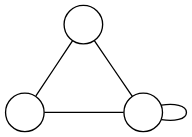
\includegraphics[width=100pt]{figures/lacan_a}
    \caption{\label{lac:a}}
  \end{subfigure}%
  \begin{subfigure}[β]{0.33\linewidth}
    \centering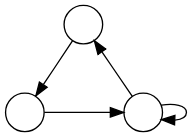
\includegraphics[width=130pt]{figures/lacan_b}
    \caption{\label{lac:b}}
  \end{subfigure}
  \begin{subfigure}[γ]{0.33\linewidth}
  \centering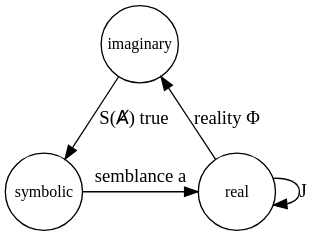
\includegraphics[width=170pt]{figures/lacan_c}
  \caption{\label{lac:c}}
  \end{subfigure}

  \caption[Παράδειγμα γράφου σε διαδοχικές πιο πλούσιες σε πληροφορία αναπαραστάσεις]{Παράδειγμα: H \textit{Λακανική τριάδα} σε διαδοχικές πιο πλούσιες σε πληροφορία αναπαραστάσεις: \subref{lac:a}: γράφος, \subref{lac:b}: κατευθυνόμενος γράφος, \subref{lac:c}: γράφος με επισημειώσεις στις ακμές και στους κόμβους}
\label{lac}
\end{figure}

Ένας γράφος με επισημειώσεις στους κόμβους του λέγεται επίσης επισημειωμένος ανά κόμβο (\en{node-labeled}).
Παρόμοια ένας γράφος με επισημειώσεις στις ακμές του λέγεται επισημειωμένος ανά ακμή (\en{edge-labeled}).
Ένας γράφος με επισημειώσεις και στους κόμβους και στις ακμές λέγεται πλήρως επισημειωμένος (βλ. σχήμα \ref{lac}\subref{lac:c}).
Στην παρούσα διπλωματική θα μας απασχολήσουν και τα τρία παραπάνω είδη επισημειωμένων γράφων. Οι επισημειώσεις μπορούν να είναι είτε διακριτές (\en{discrete}) είτε συνεχής (\en{continuous}).
Οι συνεχείς επισημειώσεις ονομάζονται και χαρακτηριστικά (\en{attributes}).

Μία εναλλακτική και πολύ κοινή αναπαράσταση της δομής ενός γράφου είναι ο πίνακας γειτνίασης (\en{adjacency matrix}).
\begin{definition}[Πίνακας γειτνίασης]
Δεδομένου ενός γράφου $G = ( V, E )$, ο πίνακας γειτνίασης του $A_{G}$ του γράφου $G$ είναι ένας δισδιάστατος πίνακας $|V|\times |V|$, όπου με $Α_{ij}$ συμβολίζουμε το στοιχείο στην \en{i}-οστή γραμμή και \en{j}-οστή στήλη του πίνακα τότε:
\begin{equation}
 A_{ij} =
\begin{cases}
1, \{v_{i}, v_{j}\} \in E\\
0, otherwise
\end{cases}
\end{equation}
\label{def:adjacency_matrix}
\end{definition}

Μία έννοια πολύ κοινή στην ορολογία των γράφων, είναι αυτή της γειτονιάς.
\begin{definition}[Γειτονιά]
Δεδομένου ενός μη κατευθυνόμενου γράφου $G = ( V, E )$ και ενός κόμβου $v_{i} \in V$,
η γειτονιά $\mathcal{N}(v_{i})$ του $v_{i}$, ορίζεται ως $\mathcal{N}(v_{i}) = \{v_{j} : \{v_{i}, v_{j}\} \in E\}$, όπου $\{v_{i}, v_{j}\}$ είναι μία ακμή μεταξύ δύο κόμβων $v_{i}$ και $v_{j}$ του $V$ και αντιστοιχεί στο σύνολο των κόμβων που συνδέονται με το $v_{i}$ μέσα στο $G$.
\end{definition}

Μία έννοια στενά συνδεδεμένη με την γειτονιά είναι ο βαθμός (\en{degree}).
\begin{definition}[Βαθμός]
Δεδομένου ενός μη κατευθυνόμενου γράφου $G = ( V, E )$ και ενός κόμβου $v_{i} \in V$, ο βαθμός του $v_{i}$ στο $G$ ορίζεται ως $$d_{G} ( v_{i} ) = |\{ v_{j} : \{ v_{i} , v_{j} \} \in E \}| = |\mathcal{N} ( v_{i} )|$$ και αντιστοιχεί στον αριθμό των κόμβων που συνδέονται με το $v_{i}$,
\end{definition}
Για κατευθυνόμενους γράφους ορίζουμε στην ίδια λογική, εισερχόμενος-βαθμός (\en{in-degree}) και εξερχόμενος-βαθμός (\en{out-degree}) για τις ακμές που εισέρχονται και εξέρχονται αντίστοιχα.
Κομβική για την θεωρία γράφων, είναι και η έννοια του υπογραφήματος.
\begin{definition}[Υπογράφημα]
Δεδομένου ενός γράφου $G = ( V, E )$, ένας γράφος $G' = ( V', E')$ θα λέγεται υπογράφημα (\en{subgraph}) του $G$ και θα συμβολίζεται με $G' \subseteq G$, αν ισχύει $V' \subseteq V$ και $E' \subseteq E$.
\label{def:subgraph}
Στην περίπτωση που το παραπάνω συνδέεται άμεσα με ένα υποσύνολο των κόμβων και όχι των ακμών, φτάνουμε στον ορισμό του επαγόμενου υπογραφήματος.
\end{definition}
\begin{definition}[Επαγόμενο Υπογράφημα]
Δεδομένου ενός γράφου $G = ( V, E )$ και ενός υποσυνόλου κόμβων $U \subseteq V$, το υπογράφημα $G(U) = (U, E(U))$ θα λέγεται επαγόμενο (\en{induced}) δεδομένου ότι οι ακμές του $E(U)$ είναι ακριβώς όλες εκείνες οι ακμές που ανήκουν στο $E$ και συνδέουν κόμβους που ανήκουν και οι δύο στο $U$, ως εξής:
\begin{equation}
    E(U) = \{\{v_{i},v_{j}\}\in E: v_{i}, v_{j}\in U\}\}
\end{equation}
\label{def:induced_subgraph}
\end{definition}
Ο βαθμός ενός κόμβου $v_{i} \in U, d_{G}(U)(v_{i})$, ισούται με τον αριθμό κόμβο που είναι γειτονικοί του $v_{i}$ στον $G(U)$.
Μία μετρική που περιγράφει συνολικά αν το πλήθος των βαθμών προσεγγίζουν το μέγιστο, είναι αυτή της πυκνότητας.
\begin{definition}[Πυκνότητα]
Δεδομένου ενός γράφου $G = ( V, E )$ ορίζουμε ως πυκνότητα (\en{density}) του γράφου $G$ τον αριθμό $\delta(G) = \frac{|E|}{|V|^{2}}$.
\end{definition}
Ένας γράφος στον οποίο ισχύει $\delta(G) = 1$, λέγεται πλήρης γράφος.
Σε ένα πλήρη γράφο κάθε ζευγάρι κορυφών συνδέονται.
Με βάση αυτή τη συνθήκη και της έννοιας του επαγόμενου υπογράφου, φτάνουμε στον ορισμό της κλίκας.
\begin{definition}[Κλίκα]
Δεδομένου ενός γράφου $G = ( V, E )$ θα ονομάζουμε κλίκα (\en{clique}) ένα υποσύνολο κόμβων $C \subseteq V$, τέτοιο ώστε $\delta(G(C)) = 1$.
\end{definition}
Θεμελιώδες έννοιες για την ανάλυση και εξερεύνηση ενός γράφου, είναι αυτές του περιπάτου, του μονοπατιού και του κύκλου.
\begin{definition}[Περίπατος, Μονοπάτι, Κύκλος]
Ένας περίπατος (\en{walk}) σε ένα γράφος $G = (V, E)$ είναι μία ακολουθία από κόμβους $v_{1}, v_{2}, \dots , v_{l + 1}$ όπου $v_{i} \in V$ για όλα τα $1 \leq i \leq l + 1$ και $\{ v_{i} , v_{i + 1} \} \in E$ για όλα τα
$1 \leq i \leq k$. To μήκος ενός περιπάτου είναι ίσο με τον αριθμό των ακμών στην ακολουθία, δηλαδή $l$.
Ένας περίπατος στον οποίο ισχύει $$v_{i} = v_{j} \Leftrightarrow i = j$$ ονομάζεται μονοπάτι (\en{path}).
Ένας κύκλος (\en{cycle}) είναι ένα μονοπάτι για το οποίο ισχύει $\{v_{k + 1}, v_{1}\} \in E$.
\label{def:path}
\end{definition}
Ενώ με βάση αυτές μπορούμε να ορίσουμε μία έννοια απόστασης για δύο κόμβους, το κοντινότερο μονοπάτι.
\begin{definition}[Κοντινότερο Μονοπάτι]
Κοντινότερο μονοπάτι (\en{shortest path}) μεταξύ δύο κόμβων $v_{i}, v_{j}$, ενός γράφου $G$ είναι ένα μονοπάτι από
το $v_{i}, v_{j}$, τέτοιο ώστε δεν υπάρχει άλλο μονοπάτι μεταξύ αυτών των δύο κορυφών με μικρότερο μήκος.
\end{definition}
\textit{Διάμετρος} ενός γράφου $G$ είναι το μήκος του μεγαλύτερου ελαχίστου μονοπατιού μεταξύ κάθε ζευγάρι κόμβων στον γράφο $G$.
Τελευταία και μη εξαιρετέα είναι η σχέση που προσδιορίζει αν δύο γράφοι ταυτίζονται, γνωστή ως ισομορφισμός.
\begin{definition}[Ισομορφισμός]
Ένας ισομορφισμός μεταξύ δύο επισημειωμένων γράφων $G=(V,E)$ και $G'=(V',E')$ είναι μία "1-1" απεικόνιση $\phi : V \rightarrow V'$ που διατηρεί τη γειτνίαση, δηλαδή $\forall v,u \in V : (v,u) \in E \Leftrightarrow (\phi(v), \phi(u)) \in E'$ και τις επισημειώσεις, δηλαδή αν $\psi \in V \times V \rightarrow V' \times V'$ είναι η αντιστοίχιση των ζευγαριών κόμβων όπως προκύπτει από την "1-1" απεικόνιση $\phi$ τέτοια ώστε $\psi((v,u)) = (\phi(v), \phi(u))$, τότε οι συνθήκες $\forall v \in V : \ell(v) \equiv \ell(\phi(v))$ και $\forall e \in E : \ell(e) \equiv \ell(\psi(e))$ πρέπει να ικανοποιούνται, όπου με $\equiv$ συμβολίζουμε ότι δύο επισημειώσεις ταυτίζονται.
\label{def:isomorphism}
\end{definition}
\section{Προβλήματα Μηχανικής Μάθησης}
Το σύνολο των προβλημάτων στον χώρο της μηχανικής μάθησης είναι τριχοτομημένο στις εξής μεγάλες κατηγορίες ($1$) επιβλεπόμενη (\en{supervised}) μάθηση, ($2$) μη-επιβλεπόμενη (\en{un-supervised}) μάθηση και ($3$) ενισχυτική (\en{reinforcement}) μάθηση. 
Στην \textit{επιβλεπόμενη} μάθηση, ο στόχος είναι η μάθηση μίας αντιστοίχισης μεταξύ εισόδου εξόδου, δεδομένου ενός συνόλου ζευγαριών τιμών εισόδου - εξόδου, γνωστό ως σύνολο εκπαίδευσης.
Στην περίπτωση που έχουμε διακριτή έξοδο, το πρόβλημα αυτό ονομάζεται \textit{πρόβλημα ταξινόμησης}.
Ένα γνωστό πρόβλημα ταξινόμησης είναι αυτό της αναγνώρισης χειρόγραφων ψηφίων.
Οι είσοδοι αντιστοιχούν σε εικόνες χειρόγραφων ψηφίων και οι έξοδοι ή αλλιώς οι \textit{επισημειώσεις} των κατηγοριών στο νούμερο του ψηφίου από το οποίο έχουν προέλθει οι αναπαραστάσεις.
Δεδομένου ενός εκπαιδευτικού συνόλου εικόνων και των κατηγορικών επισημειώσεων τους, ο στόχος είναι η μάθηση μία αντιστοίχισης από εικόνες σε κατηγορικές επισημειώσεις, που μπορούν να χρησιμοποιηθούν για να αναγνωρίσουμε σε ποια κατηγορία ανήκουν νέες εικόνες.
Αν η έξοδος αποτελείται από μία ή παραπάνω συνεχείς μεταβλητές, το πρόβλημα είναι γνωστό ως πρόβλημα παλινδρόμησης (\en{regression}).
Ένα παράδειγμα ενός τέτοιου προβλήματος μπορεί να είναι το εξής: δεδομένου ψυχοφυσικών επισημειώσεων σχετικά με το αν μία μουσική μελωδία είναι αγχωτική με συνεχείς μετρήσεις από το $0$ έως το $5$, πρόβλεψη του βαθμού άγχους που προκαλεί μία μελωδία, έχοντας ως είσοδο ένα συνόλο χαρακτηριστικών που εξάγουμε από το ηχητικό (ή μελωδικό) της σήμα.
Στην \textit{μη-επιβλεπόμενη} μάθηση, μας δίνονται μόνο είσοδοι και ο στόχος μας είναι να εξάγουμε χρήσιμα πρότυπα (\en{patterns}) από αυτές.
Ένα παράδειγμα μη επιβλεπόμενης μάθησης είναι η συσταδοποίηση (\en{clustering}), που αφορά τον διαχωρισμό των δεδομένων εισόδου σε ομάδες, έτσι ώστε τα δεδομένα εισόδου που καταλήγουν να είναι στην ίδια ομάδα, να είναι κατά μία έννοια πιο όμοια μεταξύ τους από αυτά που ανήκουν σε άλλες ομάδες.
Άλλο ένα πρόβλημα, γνωστό ως εκτίμηση πυκνότητας (\en{density estimation}) αφορά τον προσδιορισμό μίας ``κρυφής'' συνάρτησης πυκνότητας πιθανότητας, δεδομένου ενός συνόλου δεδομένων εισόδου.
Τέλος, όσον αφορά την \textit{ενισχυτική} μάθηση, στόχος είναι να προσδιορίσουμε ποιες δράσεις πρέπει να λάβουμε σε μία δεδομένη κατάσταση προκειμένου να μεγιστοποιήσουμε μία μετρική που ποσοτικοποιεί κάποια έννοια συνολικής ανταμοιβής.
Σε αντίθεση με την επιτηρούμενη μάθηση, οι ιδανικές έξοδοι δεν είναι γνωστές εξαρχής, αλλά αποκαλύπτονται την ώρα της ίδιας της διαδικασίας μάθησης καθώς το σύστημα αλληλεπιδρά με ένα άλλο σύστημα-περιβάλλον, το οποίο το ανταμείβει ή όχι με βάση την κατάσταση του κάθε στιγμή.
\subsection{Προβλήματα Μάθησης με Γράφους}
Η μάθηση σε γράφους έχει συγκεντρώσει μεγάλο ερευνητικό ενδιαφέρον τα τελευταία χρόνια.
Όπως σχολιάστηκε παραπάνω, λόγω των υψηλών αναπαραστατικών δυνατοτήτων τους, οι γράφοι χρησιμοποιούνται για να αναπαραστήσουν δεδομένα από πολύ διαφορετικές πηγές.
Ως επακόλουθο δεν μας εκπλήσσει το γεγονός ότι μία πληθώρα προβλημάτων μάθησης είναι ορισμένα για γράφους.
Τα ακόλουθα τέσσερα προβλήματα είναι ίσως αυτά που έχουν μελετηθεί περισσότερο στην βιβλιογραφία:
\begin{itemize}
\item Ταξινόμηση Κόμβων: δεδομένου ενός γράφου με επισημειώσεις σε ένα γνήσιο υποσύνολο των κόμβων, επισημείωσε αποτελεσματικά τους υπόλοιπους.
\item Πρόβλεψη σύνδεσης: δεδομένου ενός συνόλου κόμβων, πρόβλεψε αν πρέπει να συνδεθούν με μία ακμή.
\item Ταξινόμηση Γράφων: δεδομένου ενός συνόλου γράφων με γνωστή κατηγοριοποίηση για ένα γνήσιο υποσύνολο τους, βρες σε ποιές κατηγορίες ανήκουν οι υπόλοιποι.
\item Συσταδοποίηση Γράφων: δεδομένου ενός γράφου, ομαδοποίησε όλους τους κόμβους του σε συστάδες, λαμβάνοντας υπόψιν την δομή των ακμών του κατά τέτοιο τρόπο ώστε να υπάρχουν πολλές ακμές εσωτερικά κάθε συστάδας, και σχετικά λίγες μεταξύ τους.
\end{itemize}
Τα τρία πρώτα προβλήματα είναι προβλήματα \textit{επιτηρούμενης} μάθησης, ενώ το τελευταίο είναι ένα πρόβλημα \textit{μη-επιτηρούμενης} μάθησης.
Στο εύρος αυτής της διπλωματικής θα μας απασχολήσει μόνο το τρίτο πρόβλημα, συγκεκριμένα αυτό της ταξινόμησης γράφων.
\subsection{Το Πρόβλημα Ταξινόμησης Γράφων}
\label{subsection:graph_classification}
Το πρόβλημα ταξινόμησης είναι το πιο συχνά εμφανιζόμενο πρόβλημα στο χώρο της μηχανικής μάθησης.
Σε ένα πρόβλημα \textit{ταξινόμησης}, στόχος είναι η μάθηση μίας αντιστοίχισης μεταξύ εισόδου-εξόδου, δεδομένου ενός συνόλου εκπαίδευσης.
Στα παρακάτω, θα συμβολίζουμε την είσοδο με $x$ και την έξοδο με $y$.
Οι είσοδοι συχνά αποκαλούνται και παραδείγματα ή στιγμιότυπα του προβλήματος, τη στιγμή που οι έξοδοι συνήθως αποκαλούνται επισημειώσεις κατηγοριών.
Στις περισσότερες περιπτώσεις, κάθε είσοδος $x$ αναπαρίσταται σαν ένα διάνυσμα πραγματικών αριθμών.
Από την άλλη θα μπορούσε να είναι οτιδήποτε π.χ. μία εικόνα, ένα κείμενο ή ένας γράφος.\par
Έστω ότι το $\mathcal{X}$ είναι ένα σύνολο αντικειμένων που θα θέλαμε να ταξινομήσουμε.
Ως επακόλουθο $x \in \mathcal{X}$.
Οι έξοδοι παίρνουν τις τιμές τους από ένα πεπερασμένο σύνολo $y \in \mathcal{Y} = {C_{1}, \dots, C_{|Y|}}$, όπου το $C$ είναι ένα πλήθος από κατηγορίες.
Αν το $|\mathcal{Υ}| = 2$ τότε το προκύπτον πρόβλημα ονομάζεται πρόβλημα \textit{δυαδικής} ταξινόμησης.
Εναλλακτικά, αν $|\mathcal{Y}| > 2$, λέγεται \textit{πολυ-κατηγορική} ταξινόμηση.
Πάντοτε σε ένα πρόβλημα ταξινόμησης μας δίνεται ένα σύνολο $\mathcal{D} = \{(x_{i}, y_{i})\}^{N}_{i=1}$ όπου $(x_{i}, y_{i}) \in \mathcal{X} \times \mathcal{Y}$, $Ν$ παρατηρήσεων μαζί με τις επισημειώσεις των κατηγοριών στις οποίες ανήκουν.
Θα υποθέσουμε ότι τα δεδομένα εκπαίδευσης $\mathcal{D}$ προέκυψαν από μία άγνωστη κατανομή.
Με βάση αυτό το σύνολο εκπαίδευσης, ο στόχος είναι να μάθουμε μία συνάρτηση $f: \mathcal{X} \rightarrow \mathcal{Y}$ που ελαχιστοποιεί το σφάλμα λανθασμένης αντιστοίχισης, δεδομένης της άγνωστης κατανομής.
Έχοντας υπολογίσει την συνάρτηση $f$, μπορούμε να την χρησιμοποιήσουμε για να κάνουμε προβλέψεις σε νέα δεδομένα.
Συνήθως μας δίνεται και ένα άλλο σύνολο ζευγαριών εισόδων-εξόδων, που περιέχει διαφορετικές εξόδους από αυτές που χρησιμοποιήθηκαν κατά την εκπαίδευση.
Αυτό το σύνολο λέγεται πειραματικό σύνολο και συνήθως χρησιμοποιείται για την εκτίμηση της ποιότητας της μάθησης.
Ιδανικά θα θέλαμε η $f$ να μπορεί να ταξινομεί σωστά νέα δείγματα.\par
Στην περίπτωση που τα δεδομένα εισόδου είναι γράφοι, το πρόβλημα λέγεται ταξινόμηση γράφων.
Συγκεκριμένα, δεδομένου ενός συνόλου εκπαίδευσης $\mathcal{D} = \{(G_{i}, y_{i})\}^{N}_{i=1}$ που αποτελείται από $N$ γράφους, στόχος είναι να μάθουμε μία συνάρτηση $f: \mathcal{G} \leftarrow \mathcal{Y}$, όπου $\mathcal{G}$ είναι ο χώρος των γράφων που μπορούν να δοθούν ως είσοδοι σε αυτήν την συνάρτηση και $\mathcal{Y}$ είναι το σύνολο των δυνατών επισημειώσεων που μπορούν να αποδοθούν στους γράφους.
Η συνάρτηση αυτή μπορεί να χρησιμοποιηθεί ύστερα για την ταξινόμηση νέων γράφων, δηλαδή γράφων που δεν εμφανίστηκαν στο σύνολο εκπαίδευσης, όπως συνήθως είναι αυτοί του πειραματικού συνόλου, σε κατηγορίες.\par
Το πρόβλημα της ταξινόμησης γράφων έχει αποτελέσει μία δημοφιλή περιοχή έρευνας τα τελευταία χρόνια, μιάς και έχει συγκεντρώσει πολλές εφαρμογές σε ένα μεγάλο εύρος περιοχών.
Τέτοιες συνοπτικά εμφανίζονται σε ένα εύρος από τον χαρακτηρισμό ενός χημικού μορίου ως μεταλλαξιογόνου \cite{Swamidass2005} και την πρόβλεψη της λειτουργίας μίας πρωτεΐνης δεδομένου της νουκλεοτιδικής του ακολουθίας \cite{Borgwardt2005}, μέχρι τον εντοπισμό του αν ένα λογισμικό είναι κακόβουλο \cite{Wagner2009}.
\subsection{Σύγκριση Γράφων}
Το πρόβλημα της ταξινόμησης γράφων συνδέεται άμεσα με αυτό της σύγκρισης.
Πολλοί αλγόριθμοι στο χώρο της μηχανικής μάθησης λαμβάνουν αποφάσεις, βάσει ενός μέτρου \textit{ομοιότητας} (\en{similarity metric}) ή ενός μέτρου \textit{απόστασης} (\en{distance metric}) μεταξύ δύο στιγμιοτύπων εισόδου.
Για παράδειγμα δημοφιλείς ταξινομητές, όπως ο ταξινομητής $k$-κοντινότερων γειτόνων ή ο ταξινομητής μηχανών διανυσμάτων υποστήριξης (βλέπε ενότητα \ref{sec:svm}), μπορούν να επιλύσουν προβλήματα μάθησης πολύ διαφορετικών δεδομένων, προσδιορίζοντας μονάχα μία μετρική ομοιότητας μεταξύ τους.
Κατ' αυτόν τον τρόπο προσδιορίζοντας μία συνάρτηση απόστασης $d : \mathcal{G} \times \mathcal{G} \rightarrow \mathbb{R}^{+}$ μεταξύ γράφων, μπορούμε άμεσα να χρησιμοποιήσουμε έναν από τους παραπάνω αλγορίθμους, για να ταξινομήσουμε δεδομένα που έχουν αναπαρασταθεί ως γράφοι.\par
Η σύγκριση γράφων είναι από μόνη της ένα πολύ δύσκολο πρόβλημα.
Συγκεκριμένα, δεδομένου δύο γράφων $G_{i}, G_{j}$ σε ένα χώρο γράφων $\mathcal{G}$, το πρόβλημα της σύγκρισης γράφων αφορά τον προσδιορισμό μίας συνάρτησης αντιστοίχισης: $f: \mathcal{G} \times \mathcal{G} \rightarrow \mathbb{R}$, τέτοια ώστε να ``ποσοτικοποιεί'' είτε μία έννοια ομοιότητας μεταξύ των γράφων $G_{i}, G_{j}$ είτε μία έννοια απόστασης μεταξύ τους (η έννοια της απόστασης είναι η αντίστροφη της ομοιότητας και συνεπώς συμπληρωματική).
Η σύγκριση γράφων είτε από μόνη της είτε στον χώρο της ταξινόμησης γράφων βρίσκει εφαρμογή σε πολλά πεδία.
Συγκεκριμένα στην χημιοπληροφορική, χρησιμοποιήθηκε για την πρόβλεψη κινητικών μοντέλων μεταξύ χημικών αντιδράσεων \cite{Genesys} και για την ταξινόμηση χημικών μορίων με στόχο π.χ. την ανίχνευση φαρμακευτικής δράσης \cite{Wale2008}.
Στην βιοπληροφορική, χρησιμοποίηθηκε για την κατάταξη γονιδίων και γονιδιωμάτων σε μία βάση γνώσης\cite{KEGG, Hattori2003} και στην κατανόηση μηχανισμών γονιδιακής ρύθμισης \cite{Davidson1669}.
Πέρα από τους δύο αυτούς τομείς, η ομοιότητα γράφων έχει χρησιμοποιηθεί για την σύγκριση ηλεκτρικών κυκλωμάτων \cite{Takashima1988}, προγραμμάτων γλώσσας \tl{C} \cite{Gitchell1999}, κειμένων \cite{Rousseau2015TextCA}, ειδησεογραφικών γεγονότων \cite{Glavas2013} αλλά και για την αυτοματοποιημένη συλλογιστική \cite{Tsivtsivadze2011} και για την αποσαφήνιση σχεσιακών οντοτήτων \cite{Hermansson2013EntityDI}.
\section{Πυρήνες Γράφων}
Οι πυρήνες γράφων (\en{graph kernels}), αποτελούν μία από τις πιο μοντέρνες τεχνικές στην ταξινόμηση γράφων.
Τεχνικές σαν αυτή παρουσιάζουν μερικές πολύ ελκυστικές στατιστικές ιδιότητες.
Παράλληλα δύνανται να συνδυάσουν την αναπαραστατική δύναμη των γράφων και τις δυνατότητες διαχωρισμού της πληροφορίας που επιτυγχάνουν οι μέθοδοι που βασίζονται σε \textit{πυρήνες}.
Συνεπώς, αποτελούν πολύ ισχυρά εργαλεία τόσο για την αντιμετώπιση του προβλήματος της ομοιότητας γράφων όσο και για την επίλυση των προβλημάτων μάθησης.
Αυτός είναι και ο κύριος λόγος που δημιουργήθηκε το συγκεκριμένο λογισμικό, για να κάνει άμεσα προσβάσιμες αυτές τις τεχνικές στο εκάστοτε στάδιο ενός προβλήματος μηχανικής μάθησης, προς επίλυση.
\subsection{Συναρτήσεις Πυρήνα}
Αρχικά παρουσιάζεται μία θεμελιώδης εισαγωγή στις συναρτήσεις πυρήνα.
\begin{definition}[\en{Gram} Μήτρα]
Δεδομένου ενός συνόλου εισόδων $x_{1}, \dots x_{N} \in \mathcal{X}$ και μία συνάρτηση $k:\mathcal{X}\times\mathcal{X}\rightarrow \mathbb{R}$, η $N \times N$ μήτρα $K$ που ορίζεται σαν:
$$K_{ij} = k(x_{i}, x_{j}) $$
ονομάζεται \en{Gram} μήτρα (\en{Gram Matrix}) ή μήτρα πυρήνα του $k$ με βάση τις εισόδους $x_{1}, \dots, x_{N}$
\label{def:kernel_matrix}
\end{definition}
Στη συνέχεια θα αναφερόμαστε στις μήτρες \en{Gram} σαν μήτρες πυρήνα.
\begin{definition}[Θετικά Ημιορισμένος Πυρήνας]
Έστω $\mathcal{X}$ ένα μη κενό σύνολο.
Μία συμμετρική μήτρα $k:\mathcal{X} \times \mathcal{X} \rightarrow \mathbb{R}$, που για όλα τα $N \in \mathbb{N}$ και όλα τα $x_{1},\dots, x_{N} \in \mathcal{X}$, παράγει μία θετικά ημιορισμένη μήτρα, θα λέγεται θετικά ημιορισμένος πυρήνας, ή απλώς πυρήνας.
\label{def:psd_km}
\end{definition}
Πρακτικά η συνάρτηση πυρήνα είναι ένα μέτρο ομοιότητας μεταξύ δύο αντικειμένων.
Οι συναρτήσεις πυρήνα μπορούν να ειδωθούν, αλλιώς σαν εσωτερικά γινόμενα μεταξύ αναπαραστάσεων αυτών των δεδομένων.
Συγκεκριμένα, για κάθε έγκυρο πυρήνα $k$ στο $\mathcal{X}\times\mathcal{X}$, υπάρχει μία συνάρτηση $\phi: \mathcal{X} \rightarrow \mathcal{H}$ που αναπαριστά τα δεδομένα σε ένα χώρο \en{Hilbert}, τέτοια ώστε:
\begin{equation}
\forall x_{i}, x_{j} \in \mathcal{X}: k(x_{i}, x_{j}) = \langle \phi(x_{i}), \phi(x_{j}) \rangle
\end{equation}
όπου το $\langle\;.\;,\;.\;\rangle$ συμβολίζει το εσωτερικό γινόμενο σε αυτόν τον χώρο \en{Hilbert}.
Ένας χώρος \en{Hilbert}, είναι ένας χώρος με εσωτερικό γινόμενο, που ικανοποιεί την συνθήκη πληρότητας ότι ``κάθε ακολουθία σημείων \en{Cauchy} που προκύπτει από αυτόν τον χώρο, συγκλίνει σε ένα σημείο σε αυτόν τον χώρο''. Ακόμα ένας χώρος \en{Hilbert} ικανοποιεί την ακόλουθη ιδιότητα γνωστή σαν ιδιότητα αναπαραγωγής (\en{reproducing}):
\begin{equation}
\forall f \in \mathcal{H}, \forall x \in \mathcal{X}: f(x)=\langle f, k(x,\dot)\rangle
\end{equation}
Λόγω αυτής της ιδιότητας, ο $\mathcal{H}$ λέγεται χώρος \en{Hilbert} αναπαραγωγικού πυρήνα (\en{reproducing kernel Hilbert space} - \en{RKHS}) και συνδέεται με τον πυρήνα $k$.
Είναι ενδιαφέρον να σημειώσουμε ότι κάθε συνάρτηση στο $\mathcal{X} \times \mathcal{X}$ συνδέεται με έναν \en{RKHS} και αντίστροφα \cite{Aronszajn1950}.

\subsection{Μέθοδοι Πυρήνα}
Οι μέθοδοι πυρήνα (\en{Kernel methods}) είναι ένα σύνολο από αλγορίθμους μηχανικής μάθησης, που λειτουργούν σε ένα σύνολο δεδομένων εισόδου τα οποία έχουν έμμεσα αναπαρασταθεί σε ένα χώρο χαρακτηριστικών (\en{feature space}) χρησιμοποιώντας μία συνάρτηση πυρήνα.
Ένα από τα σημαντικότερα πλεονεκτήματα αυτών των μεθόδων είναι ότι λειτουργούν σε πολλά και διαφορετικά είδη δεδομένων \cite{ScholkopfSmolaLK}.
Ο χώρος εισόδων $\mathcal{X}$, δεν χρειάζεται να είναι ένας διανυσματικός χώρος, αλλά μπορεί να αναπαριστά οποιαδήποτε κατηγορία δεδομένων, όπως τον χώρο των συμβολοσειρών (\en{string}) ή τον χώρο των γράφων \cite{GartnerSKSD}.
Οι μέθοδοι πυρήνα μπορούν ακόμα να εφαρμοσθούν σε πολλούς τύπους δεδομένων, από την στιγμή που μπορούμε να βρούμε μία αναπαράσταση $\phi : \mathcal{X} \rightarrow \mathcal{H}$, όπου το $\mathcal{H}$ είναι ένας \en{RKHS}.
Μία τέτοια αναπαράσταση δεν είναι αναγκαίο να είναι φανερά ορισμένη.
Οι μέθοδοι αυτοί κατά την εκτέλεση των υπολογισμών τους, αναπαριστούν έμμεσα τα δεδομένα σε ένα χώρο χαρακτηριστικών, υπολογίζοντας την τιμή του εσωτερικού γινομένου που θα είχαν αυτές οι αναπαραστάσεις αν ήταν φανερές σε αυτό τον χώρο, κάνοντας χρήση μίας συνάρτησης πυρήνα.
Τέτοια εσωτερικά γινόμενα μπορούν να ερμηνευτούν ως μέτρα ομοιότητας μεταξύ των αντίστοιχων αντικειμένων, που συγκρίνουν.
Προβλήματα μηχανικής μάθησης όπως η ταξινόμηση και η συσταδοποίηση, μπορούν να έρθουν εις πέρας χρησιμοποιώντας μόνο εσωτερικά γινόμενα που έχουν υπολογιστεί σε τέτοιους μη-φανερούς χώρους χαρακτηριστικών.\par
Οι μέθοδοι πυρήνα είναι πολύ δημοφιλείς και έχουν φανεί ιδιαίτερα επιτυχημένες σε ένα μεγάλο σύνολο εφαρμογών.
Για να διασαφηνίσουμε λίγο περισσότερο τα παραπάνω, ας θεωρήσουμε ένα πρόβλημα δυαδικής ταξινόμησης, με ένα σύνολο εκπαίδευσης $D = \{( x_{i}, y_{i})\}^{Ν}_{i = 1}$ όπου $(x_{i}, y_{i}) \in \mathcal{X} \times \mathcal{Y}$ και ο $\mathcal{X}$ είναι ένας χώρος με εσωτερικό γινόμενο (π.χ. $R^{d}$) και $Y = \{-1, +1\}$.
Όπως αναφέρθηκε και παραπάνω, δεδομένου ενός συνόλου εκπαίδευσης $D$, στόχος είναι η \textit{μάθηση} μίας συνάρτησης $f : \mathcal{X} \rightarrow \mathcal{Y}$, τέτοια ώστε το σφάλμα γενίκευσης της $f$ είναι όσο το δυνατόν χαμηλότερο.
Συνεπώς αυτό που μας ενδιαφέρει είναι να ελαχιστοποιήσουμε το σφάλμα εκπαίδευσης, διατηρώντας ταυτόχρονα μία καλή απόδοση στα νέα δεδομένα (αυτά που δεν εμφανίστηκαν στο σύνολο εκπαίδευσης).
Η κύρια τέτοια μέθοδος που θα μας απασχολήσει (βλ. ενότητα \ref{sec:svm}), ανήκει στις μεθόδους μεγάλου περιθωρίου (\en{large margin methods}), οι οποίες αναζητούν ένα υπερεπίπεδο που διαχωρίζει το μέρος των δειγμάτων εκπαίδευσης που ανήκουν στην κατηγορία $-1$ από αυτά που ανήκουν στην κατηγορία $1$.
Εν συνεχεία, η $f$ μπορεί να πάρει την μορφή $f(x) = \sign (\langle w, x \rangle + b )$, όπου η συνάρτηση $\sign(\dot)$ αντιστοιχεί στην συνάρτηση προσήμου (η οποία παίρνει την τιμή $1$ αν το όρισμα της είναι θετικό και την τιμή $-1$ αλλιώς).
Δεδομένου ενός $x$, η \textit{συνάρτηση απόφασης} $f$ δίνει στην έξοδο της μία πρόβλεψη που εξαρτάται από την θέση του $x$ σε σχέση με το υπερεπίπεδο $\langle w, x \rangle + b = 0$.\par
Αρχικά, ας υποθέσουμε ότι τα δεδομένα εκπαίδευσης είναι γραμμικά διαχωρίσιμα.
Αν κάτι τέτοιο συμβαίνει, υπάρχει ένα υπερεπίπεδο τέτοιο ώστε τα σημεία που ανήκουν σε διαφορετικές κλάσεις βρίσκονται στις αντίθετες πλευρές του.
Στην πραγματικότητα, παρουσιάζεται απειρία τέτοιων υπερεπιπέδων.
Οι ταξινομητές μεγάλου περιθωρίου, επιλέγουν μεταξύ αυτών των υπερεπιπέδων αυτό που μεγιστοποιεί το περιθώριο μεταξύ των δύο κατηγοριών των σημειακών δεδομένων εκπαίδευσης, αυτό δηλαδή για το οποίο η απόσταση από τα κοντινότερα δεδομένα των δύο κατηγοριών είναι μέγιστη.
Για την εύρεση αυτού του βέλτιστου υπερεπιπέδου, αναγκαία είναι η λύση ενός προβλήματος κυρτής τετραγωνικής βελτιστοποίησης.
Το διάνυσμα $w$ που προκύπτει ως λύση σε αυτό το πρόβλημα είναι ένας γραμμικός συνδυασμός των παραδειγμάτων εκπαίδευσης:
\begin{equation}
w = \sum_{i=1}^{N}a_{i}y_{i}x_{i}
\end{equation}
όπου το $\alpha_{i} \in \mathbb{R}^{+}$.

Χρησιμοποιώντας το παραπάνω αποτέλεσμα, που είναι γνωστό ως το θεώρημα αναπαράστασης (\en{representer theorem}) \cite{ScholkopfGRT}, ο γραμμικός ταξινομητής $f$ μπορεί να γραφεί ως:
\begin{equation}
f(x) = \sign ( \sum_{i=1}^{N} α_{i}y_{i} \langle x_{i} , x \rangle + b )
\end{equation}

Στην περίπτωση, τώρα, που τα δεδομένα εκπαίδευσης δεν είναι γραμμικά διαχωρίσιμα, αναζητούμε ένα υπερεπίπεδο που μεγιστοποιεί το περιθώριο και την ίδια στιγμή ελαχιστοποιεί μία ποσότητα αντιστρόφως ανάλογη στο πλήθος των λαθών ταξινόμησης.
Ο υπολογισμός αυτού του υπερεπιπέδου μπορεί και πάλι να διατυπωθεί ως ένα πρόβλημα κυρτής τετραγωνικής βελτιστοποίησης, όπου το διάνυσμα λύσης $w$ συνεχίζει να προκύπτει ως ένας γραμμικός συνδυασμός των δεδομένων εισόδου.\par
Σε σύνθετα προβλήματα ταξινόμησης, είναι πιθανό να μην υπάρχουν υπερεπίπεδα τέτοια ώστε να διαχωρίζουν τα θετικά επισημειωμένα παραδείγματα από τα αρνητικά, με τέτοιο τρόπο ώστε να παρέχουν ένα καλό αποτέλεσμα ταξινόμησης.
Η απάντηση σε αυτό το πρόβλημα, που συχνά είναι γνωστή ως τέχνασμα πυρήνα (\en{kernel trick}: \cite{Aizerman67theoretical, Boser1992}), είναι η απεικόνιση των δεδομένων εισόδου σε έναν άλλο χώρο χαρακτηριστικών $\mathcal{H}$ (συνήθως υψηλότερων διαστάσεων) και η εύρεση ενός διαχωριστικού υπερεπιπέδου σε αυτόν τον χώρο.
Έστω $\mathcal{\phi} : \mathcal{X} \rightarrow \mathcal{H}$ μία απεικόνιση από το $\mathcal{X}$ στο χώρο χαρακτηριστικών $\mathcal{H}$, που διαθέτει εσωτερικό γινόμενο.
Για να υπολογίσουμε το βέλτιστο υπερεπίπεδο στο χώρο χαρακτηριστικών, μπορούμε να χρησιμοποιήσουμε την προηγούμενη μαθηματική διατύπωση, απλώς αντικαθιστώντας το $\langle x_{i} , x \rangle$ με $\langle \phi(x_{i}), φ(x) \rangle$.
Έστω $k : \mathcal{X} \times \mathcal{X} \rightarrow \mathbb{R}$ μία συνάρτηση πυρήνα με την ακόλουθη ιδιότητα:
\begin{equation}
k(x_{i}, x_{j}) = \langle \phi (x_{i}), \phi (x_{j}) \rangle    
\end{equation}
Η συνάρτηση απόφασης $f$ μπορεί, τώρα, να γραφτεί ως:
\begin{equation}
f(x) = \sign(\sum_{i=1}^{N}\alpha_{i} y_{i} \langle \phi(x_{i}), \phi(x) \rangle + b ) = \sign(\sum_{i=1}^{N}\alpha_{i}y_{i} k(x_{i}, x) + b)
\end{equation}
Από την παραπάνω ανάλυση, είναι φανερό ότι ορίζοντας μία συνάρτηση πυρήνα $k$, απεικονίζουμε έμμεσα όλα τα σημεία των δεδομένων σε ένα χώρο χαρακτηριστικών $\mathcal{H}$. 
Ως επακόλουθο οι μέθοδοι πυρήνα μπορούν να λύσουν προβλήματα μηχανικής μάθησης, όπως η ταξινόμηση, χωρίς να χρειάζεται πουθενά, να διατυπώσουν ρητά μία τέτοια αντιστοίχιση.

\section{Μηχανή Διανυσμάτων Υποστήριξης}
\label{sec:svm}
Στη συνέχεια θα αναλύσουμε την μέθοδο πυρήνα του ταξινομητή μηχανής διανυσμάτων υποστήριξης (\en{support vector machine} ή αλλιώς \en{SVM}), ένα από τους πιο δημοφιλείς αλγορίθμους μηχανικής που έχει ως βάση του πυρήνες.
Ο κλασσικός ταξινομητής \en{SVM}, θέτει το ακόλουθο πρόβλημα: δεδομένου ενός συνόλου $N$ αντικειμένων εκπαίδευσης, μαζί με τις κατηγορίες τους $D = \{(x_{i}, y_{i})\}_{i=1}^{N}, x_{i} \in \mathcal{X}=\mathbb{R}^{d}, y_{i} \in \mathcal{Y} = \{-1, +1\}$, υπολόγισε ένα ταξινομητή $f : \mathcal{X} \to \mathcal{Y}$ που προβλέπει τις κατηγορίες νέων δεδομένων.
Στην διατύπωση των προβλημάτων \textit{άκαμπτου ορίου} (\en{hard margin}), θεωρούμε πώς τα προβλήματα μας είναι γραμμικά διαχωρίσιμα.\par
Όντας στην οικογένεια των ταξινομητών μεγάλου περιθωρίου, ο \en{SVM} αναζητά ένα υπερεπίπεδο που διαχωρίζει στιγμιότυπα της κατηγορίας $-1$ από την κατηγορία $+1$ \cite{vapnik1963}.
Έστω $(w, b)$ οι παράμετροι του υπερεπιπέδου.
Τότε, η απόσταση μεταξύ ενός σημείου $x\in \mathbb{R}^{d}$ και του υπερεπιπέδου υπολογίζεται ως:
\begin{equation}
    \frac{|w^{T}x+b|}{||w||}
\end{equation}
Αξίζει σε αυτό το σημείο να επισημάνουμε πως, ένα υπερεπίπεδο είναι αναλλοίωτο σε έναν μη-μηδενικό βαθμωτό πολλαπλασιασμό.
Ως επακόλουθο μπορούμε να θέσουμε τις παραμέτρους του υπερεπιπέδου σε συγκεκριμένες τιμές έτσι ώστε να ισχύει ως προς το υπερεπίπεδο:
$w^{Τ}x + b = 1$ και $w^{Τ}x + b = -1$ για το κοντινότερο θετικό και κοντινότερο αρνητικό δείγμα, αντίστοιχα.
Τότε, η απόσταση μεταξύ δύο σημείων από το υπερεπίπεδο (δηλ. το περιθώριο) είναι ίσο με:
\begin{equation}
    \frac{1}{||w||}
\end{equation}
Ως επακόλουθο, η μεγιστοποίηση του περιθωρίου συνεπάγεται ελαχιστοποίηση του $||w||$, πράγμα που είναι ισοδύναμο με την ελαχιστοποίηση του $\frac{1}{2}||w||^{2}$.
Συνεπώς στην περίπτωση που τα δεδομένα είναι διαχωρίσιμα, η λύση του \en{SVM} είναι η λύση του ακόλουθου προβλήματος ελαχιστοποίησης:
\begin{equation*}
\begin{aligned}
& \underset{w, b}{\text{\en{minimize}}}
& & \frac{1}{2}||w||^{2} \\
& \text{\en{subject to}}
& & y_{i}(\langle w, \; x_{i}\rangle + b) \geq 1 \; \forall i \in \{1,\dots,N\}
\end{aligned}
\end{equation*}
που αποτελεί ένα πρόβλημα κυρτού προγραμματισμού με περιορισμούς \cite{Boyd2004}.
Αν τώρα στραφούμε στο δυϊκό (κατά \en{Lagrange}) αυτού του προβλήματος:
\begin{equation}
\begin{aligned}
& \underset{\alpha}{\text{\en{maximize}}}
& & \sum_{i=1}^{N}\alpha_{i} -\frac{1}{4}\sum_{i=1}^{N}\sum_{j=1}^{N}\alpha \\
& \text{\en{subject to}}
& & \sum_{i=1}^{N}\alpha_{i}y_{i}=0\\
& & & \alpha_{i}\geq0 \; \forall i \in \{1,\dots,N\}
\end{aligned}
\label{eq:svm_basique}
\end{equation}
βλέπουμε ότι είναι δέσμιο γραμμικών περιορισμών και ως επακόλουθο έχει αποδοτική λύση, μέσω της χρήσης υπαρχόντων αλγορίθμων τετραγωνικού προγραμματισμού.
\par
Ακόμα ισχύει το εξής:
\begin{equation}
    w = \sum_{i=1}^{N} a_{i}y_{i}x_{i}
\end{equation}
Η παράμετρος $w$ του υπερεπιπέδου (δηλ. η λύση του \en{SVM}) είναι ένας γραμμικός συνδυασμός των σημείων εκπαίδευσης $x_{1} \dots x_{N}$.
Ένα σημείο $x_{i}$ συμβάλλει στην διαμόρφωση του $w$ αν και μόνον αν $α_{i} > 0$.
Για εκείνα τα σημεία δεδομένων $x_{i}$ που ικανοποιούν το $a_{i} > 0$, ισχύει ότι $y_{i}(\langle w, x_{i} \rangle + b) = 0$.
Κάτι τέτοιο σημαίνει ότι αυτά τα σημεία βρίσκονται πάνω στο περιθώριο και κατ' αυτόν τον τρόπο \textit{υποστηρίζουν} το υπερεπίπεδο.
Τα σημεία αυτά ονομάζονται \textit{διανύσματα υποστήριξης} (βλέπε σχήμα \ref{fig:svm_sep}).\par
Μέχρι στιγμής, έχουμε υποθέσει ότι τα δεδομένα εκπαίδευσης είναι γραμμικά διαχωρίσιμα.
Από την άλλη, σε μία πληθώρα πραγματικών εφαρμογών κάτι τέτοιο δεν συμβαίνει.
Για την επίλυση αυτού του προβλήματος, η συχνά αποκαλούμενη διατύπωση "εύκαμπτου ορίου" (\en{soft margin}) επιτρέπει κάποια σημεία εκπαίδευσης να μην ταξινομηθούν σωστά \cite{Bennet2002, Cortes1995}.
Συγκεκριμένα στην συνάρτηση που πρόκειται να ελαχιστοποιηθεί προστίθεται ένας όρος ποινής (\en{penalty term}) για κάθε σημείο που έχει ταξινομηθεί λάθος.
Έτσι, όσο μεγαλύτερη είναι η απόσταση ενός σημείου από το όριο, τόσο μεγαλύτερος θα είναι και ο όρος ποινής.
Επιτρέποντας λανθασμένη ταξινόμηση των δεδομένων εισόδου, είναι προφανές ότι δεν μπορούμε να χρησιμοποιήσουμε την διατύπωση του \en{SVM} όπως δόθηκε στην εξίσωση \ref{eq:svm_basique}, μιας και ο περιορισμός της δεν ικανοποιείται για τα δεδομένα που κατηγοριοποιούνται λανθασμένα.
Ως επακόλουθο, εισάγουμε μία βοηθητική μεταβλητή $\zeta_{i}$ για κάθε δεδομένο εκπαίδευσης $x_{i}$.
Η βοηθητική αυτή μεταβλητή, υπολογίζει το βαθμό που ένα σημειακό δεδομένο παραβιάζει το όριο του περιθωρίου.
Για τα σημεία των δεδομένων που βρίσκονται πάνω ή μέσα στο περιθώριο, ισχύει ότι $\zeta = 0$, ενώ για τα άλλα ισχύει:
\begin{equation}
\zeta_{i} = | y_{i} - (\langle w, x_{i} \rangle + b )|    
\end{equation}
Συνεπώς, ένα σημειακό δεδομένο $x_{i}$ που βρίσκεται πάνω στο διαχωριστικό υπερεπίπεδο θα έχει $\zeta_{i} = 1$ και τα σημεία που είναι λανθασμένα ταξινομημένα θα έχουν $\zeta_{i} > 1$ (παράβαλε σχήμα \ref{fig:svm_sep}).
\begin{figure}
    \centering
    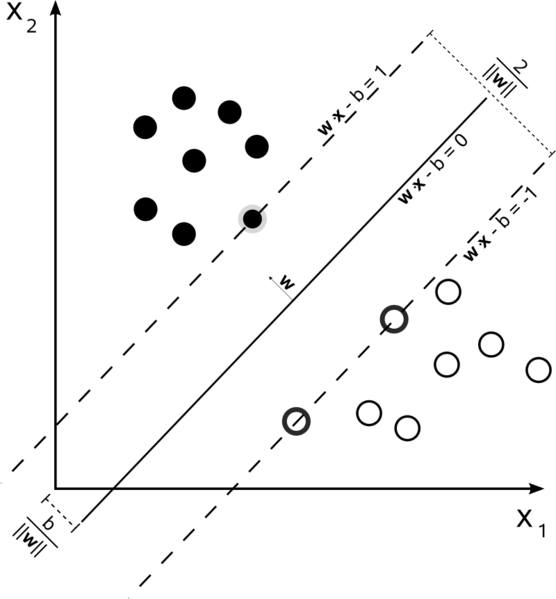
\includegraphics[scale=0.6]{figures/556px-Svm_max_sep_hyperplane_with_margin.png}
    \caption[Υπερεπίπεδο μέγιστου περιθωρίου στην περίπτωση δύο διαστάσεων για ένα \en{SVM}.]{Υπερεπίπεδο μέγιστου περιθωρίου στην περίπτωση δύο διαστάσεων για ένα \en{SVM}. Τα δείγματα που βρίσκονται στο όριο του περιθωρίου λέγονται \textbf{διανύσματα υποστήριξης}.}
    \label{fig:svm_sep}
\end{figure}
Σε τούτη την διατύπωση, στόχος μας είναι να μεγιστοποιήσουμε το περιθώριο, ενώ ταυτόχρονα μας ενδιαφέρει να ελέγξουμε την απόσταση μεταξύ των σημείων που έχουν ταξινομηθεί λάθος και του ορίου του περιθωρίου.
Η απόσταση αυτή αντιστοιχεί στην συνολική συνεισφορά των βοηθητικών μεταβλητών, που είναι ίση με $\sum_{i=1}^{N} \zeta_{i}$.
Κάτι τέτοιο μας οδηγεί στο ακόλουθο πρόβλημα βελτιστοποίησης:
\begin{equation}
\begin{aligned}
& \underset{w, b, \zeta}{\text{\en{minimize}}}
& & \frac{1}{2}||w||^{2} + C\sum_{i=1}^{N}\zeta_{i} \\
& \text{\en{subject to}}
& & y_{i}(\langle w, x_{i} \rangle + b) \geq 1 - \zeta_{i} \;\; \forall i \in \{1, \dots, N\}\\
& & & \zeta_{i} \geq 0 \; \; \forall i \in \{1, \dots, N\}
\end{aligned}
%\label{eq:svm_soft}
\end{equation}
όπου η παράμετρος $C>0$ ελέγχει το βαθμό που ο ταξινομητής πρέπει να αποφύγει να ταξινομήσει λανθασμένα ένα δείγμα εκπαίδευσης, ελέγχοντας το αντίβαρο μεταξύ μεγιστοποίησης του περιθωρίου και ελαχιστοποίησης του βάρους των βοηθητικών μεταβλητών.
Η βέλτιστη παράμετρος $C$ προσδιορίζεται συνήθως από αναζήτηση σε ένα εύρος διακριτών τιμών (\en{grid-search}) μέσω \textit{$n$-πλάσιας διασταυρωμένης επικύρωσης} (\en{n-fold cross-validation}).
Σε αυτήν την περίπτωση το δυϊκό (κατά \en{Lagrange}) πρόβλημα μπορεί να διατυπωθεί ως εξής:
\begin{equation}
\begin{aligned}
& \underset{\alpha}{\text{\en{maximize}}}
& & \sum_{i=1}^{N}\alpha_{i} -\frac{1}{4}\sum_{i=1}^{N}\sum_{j=1}^{N}\alpha \\
& \text{\en{subject to}}
& & \sum_{i=1}^{N}\alpha_{i}y_{i}=0 \\
& & & C \geq \alpha_{i}\geq0 \; \;\forall i \in \{1,\dots,N\}
\end{aligned}
\label{eq:svm_soft}
\end{equation}
Το παραπάνω πρόβλημα βελτιστοποίησης είναι κατά ενδιαφέρον τρόπο το ίδιο με την εξίσωση \ref{eq:svm_basique}, αν προσθέσουμε απλώς το $C$ ως άνω φράγμα στις παραμέτρους $\alpha_{i}$.
\section{Πυρήνες Γράφων}
Οι πυρήνες γράφων έχουν πρόσφατα προκύψει σαν μία πολλά υποσχόμενη προσέγγιση στην μηχανική μάθηση σε δεδομένα που εμφανίζονται με την μορφή των γράφων.
Αυτές οι μέθοδοι καταφέρνουν να επεκτείνουν την εφαρμοσιμότητα των μεθόδων πυρήνα στον χώρο των γράφων.
Οι πυρήνες γράφων μπορούν να χωριστούν σε δύο κατηγορίες: ($1$) αυτούς που συγκρίνουν κόμβους του ίδιου γράφου και ($2$) αυτούς που συγκρίνουν γράφους.
Οι πυρήνες που αναπτύχθηκαν στο λογισμικό της παρούσας διπλωματικής βρίσκονται αποκλειστικά στην δεύτερη κατηγορία και έτσι οπουδήποτε συναντάμε αυτόν τον όρο στα παρακάτω αυτός θα περιγράφει συναρτήσεις πυρήνα μεταξύ γράφων.\par
Από τα προηγούμενα πρέπει να είναι πλέον φανερό ότι η εφαρμογή των συναρτήσεων πυρήνα αποτελείται από δύο στάδια.
Πρώτα, σχεδιάζεται μία συνάρτηση πυρήνα, και βάση αυτής κατασκευάζεται ο πίνακας πυρήνα.
Έπειτα, ένας αλγόριθμος μάθησης χρησιμοποιείται για τον υπολογισμό μίας βέλτιστης πολλαπλότητας (\en{manifold}) στον χώρο χαρακτηριστικών (π.χ. ένα υπερεπίπεδο σε ένα πρόβλημα δυαδικού προγραμματισμού).
Από την στιγμή που υπάρχουν διάφοροι ταξινομητές ώριμοι και διαθέσιμοι στη βιβλιογραφία, οι οποίοι χρησιμοποιούν στην βάση τους πυρήνες, η έρευνα στον χώρο των πυρήνων γράφων έχει επικεντρωθεί στο πρώτο στάδιο.
Σαν επακόλουθο, το ερευνητικό έργο εστιάστηκε στην ανάπτυξη εκφραστικών και αποδοτικών πυρήνων γράφων, ικανών να μετρήσουν με ακρίβεια μία έννοια ομοιότητας.
Και στην περίπτωση αυτών των πυρήνων οι γράφοι προβάλλονται έμμεσα σε ένα χώρο χαρακτηριστικών $\mathcal{H}$.
Όσον αφορά το δεύτερο στάδιο, για το σώμα της παρούσας διπλωματικής και για την πειραματική αξιολόγηση του λογισμικού (βλ. Κεφάλαιο \ref{chap4}), θα μας απασχολήσει μόνο ο ταξινομητής $\en{SVM}$ που αναφέρθηκε παραπάνω.\par
Ο κύριος στόχος στην εφαρμογή μεθόδων πυρήνα σε γράφους είναι ο προσδιορισμός κατάλληλων θετικά ημιορισμένων συναρτήσεων πυρήνα σε ένα σύνολο δεδομένων εισόδου που δύνανται να υπολογίσουν την ομοιότητα μεταξύ τους.
Πόσο εκφραστικός μπορεί όμως να είναι ένας πυρήνας στην πράξη;
Ας υποθέσουμε αρχικά ότι ένας πυρήνας δύναται να ξεχωρίσει μεταξύ όλων των (μη-ισομορφικών) γράφων στον χώρο χαρακτηριστικών.
Ένας τέτοιος πυρήνας λέγεται \textit{πλήρης}.
\begin{definition}[Πλήρης Πυρήνας Γράφων]
Ένας πυρήνας γράφων $k(G_{i}, G_{j}) = \langle \phi (G_{i}) ,  \phi(G_{j})\rangle$ είναι πλήρης αν η $\phi$ είναι "1-1".
\end{definition}
Οι \en{Gärtner, Flach} και \en{Wrobel} έδειξαν ότι υπολογίζοντας οποιονδήποτε πλήρη πυρήνα γράφων είναι τουλάχιστον τόσο δύσκολο όσο να αποφασίσουμε αν δύο γράφοι είναι ισομορφικοί (βλέπε ορισμό \ref{def:isomorphism}) \cite{Gartner03ongraph}.
Ως αποτέλεσμα, είναι αδύνατη η χρήση πυρήνων γράφων που είναι πλήρεις σε πρακτικές εφαρμογές.
Αντίθετα, χρησιμοποιώντας πυρήνες που δεν είναι πλήρεις, δεν υπάρχει περαιτέρω εγγύηση ότι δύο μη-ισομορφικοί γράφοι δεν θα απεικονιστούν στο ίδιο σημείο στον χώρο χαρακτηριστικών.\par
Μία από τις πιο δημοφιλείς μεθόδους για να ορίσουμε πυρήνες μεταξύ σύνθετων αντικειμένων είναι να τα αποσυνθέσουμε σε πιο απλά αντικείμενα άλλου τύπου (π.χ. συμβολοσειρές, διανύσματα, ...) με γνωστούς πυρήνες και συγκρίνοντας έπειτα αυτά και συλλέγοντας τα αποτελέσματα της σύγκρισης τους με ένα κατάλληλο τρόπο, να φτιάξουμε τελικά έναν πυρήνα για τα αρχικά αντικείμενα.
Από τα πιο κοινά ήδη πυρήνων στη βιβλιογραφία, που προκύπτουν ακολουθώντας την παραπάνω μεθοδολογία λέγονται \en{R}-συνελικτικοί πυρήνες (\en{R-convolutional kernels}) \cite{Haussler1999ConvolutionKO}.
Αυτοί οι πυρήνες αποσυνθέτουν τους γράφους σε ένα σύνολο υπο-δομών και προσθέτουν τις τιμές ομοιότητας, όπως υπολογίζονται μεταξύ κάθε ζευγαριού τους.
Φυσικά θα περίμενε κανείς πως μία κατάλληλη τέτοια υπο-δομή θα ήταν οι ίδιοι οι υπογράφοι (βλέπε ορισμό \ref{def:subgraph}).
Οι \en{Gärtner, Flach} και \en{Wrobel} έδειξαν επιπρόσθετα ότι το πρόβλημα υπολογισμού ενός πυρήνα που συγκρίνει όλους τους υπογράφους είναι και αυτό \en{NP}-δύσκολο.
Κατά συνέπεια, γίνεται σαφές ότι χρειάζεται να σκεφτούμε μία εναλλακτική: λιγότερο δυνατούς πυρήνες γράφων, που είναι υπολογίσιμοι σε πολυωνυμικό χρόνο.\par
Από την άλλη, είναι απαραίτητο ότι αυτοί οι πυρήνες θα αποτελούν μία εκφραστική μετρική της \textit{ομοιότητας} μεταξύ των γράφων.
Είναι κοινό στην βιβλιογραφία οι πυρήνες να οργανώνονται σε μεγάλες κατηγορίες, που η κάθε μία μελετάει διαφορετικά δομικά χαρακτηριστικά ενός γράφου.
Συγκεκριμένα, υπάρχουν πυρήνες που συγκρίνουν γράφους, βάση τυχαίων περιπάτων \cite{gartner2003graph, borgwardt2005protein, vishwanathan2010graph}, υποδέντρων \cite{Ramon03expressivityversus, Bach2008, Mahe2009}, κύκλων \cite{Horvath2004}, μονοπατιών \cite{Borgwardt2005, Giscard2017} και μικρούς υπογράφους \cite{Costa2010, Hido2009, Kriege2012SubgraphMK, shervashidze2009efficient}.
Άλλοι αλγόριθμοι αποσυνθέτουν τους γράφους σε σύνολα από κατευθυνόμενα ακυκλικά γραφήματα (ΚΑΓ) και έπειτα χρησιμοποιώντας υπάρχοντες πυρήνες δέντρων συγκρίνουν αυτά τα ΚΑΓ μεταξύ τους \cite{Martino2006}.
Συμπληρωματικά έχουν εμφανιστεί στην βιβλιογραφία πυρήνες γράφων, που χρησιμοποιούν άλλους πυρήνες (όπως τους προαναφερθείς) που είναι γνωστοί ως σκελετοί πυρήνα (\en{kernel frameworks}).
Ο σκελετός πυρήνα \en{Weisfeiler-Lehman} βελτιώνει έτσι την απόδοση υπαρχόντων πυρήνων χρησιμοποιώντας μία επαναληπτική διαδικασία επισημείωσης των κόμβων που βασίζεται στο τεστ ισομορφισμού \en{Weisfeiler-Lehman} \cite{shervashidze2011weisfeiler}.
Ο σκελετός πυρήνα \en{k-core} αποσυνθέτει κάθε γράφο σε ιεραρχίες ένθετων υπογραφημάτων, καθένα από τα οποία παρουσιάζει μεγαλύτερο βαθμό \textit{συνδεσιμότητας} (\en{connectivity}) σε σχέση με το προηγούμενο και έπειτα κάνοντας χρήση ενός άλλου πυρήνα γράφων υπολογίζει την ομοιότητα ως το άθροισμα των ομοιοτήτων μεταξύ των υπογράφων που προκύπτουν σε κάθε επίπεδο της ιεραρχίας \cite{nikolentzos2018}.\par
Οι περισσότεροι από τους προαναφερθέντες πυρήνες γράφων συγκρίνουν συγκεκριμένες υπο-δομές των γράφων (π.χ. γραφίδια (\en{graphlets}), κύκλους, υποδέντρα κλπ).
Αυτές οι υπο-δομές αντιστοιχούν είτε σε μικρούς υπογράφους είτε σε σχέσεις μεταξύ πολύ μικρών υποσυνόλων από κόμβους.
Κατά συνέπεια οι αλγόριθμοι αυτοί εστιάζουν σε \textit{τοπικές ιδιότητες} των γράφων.
Κάποιοι πυρήνες γράφων που ξεφεύγουν από αυτήν την προσέγγιση και προσπαθούν να συγκεντρώσουν γενικά χαρακτηριστικά ή ιδιότητες των γράφων, έχουν προταθεί στη βιβλιογραφία.
Για παράδειγμα πυρήνες που βασίζονται στο αριθμό \en{Lovász} και την αντίστοιχη ορθοκανονική αναπαράσταση του γράφου \cite{johansson2014global} ή πυρήνες που χρησιμοποιούν μετρικές από την θεωρία πληροφοριών όπως την απόκλιση (\en{divergence}) \en{Jensen Shannon} \cite{Bai12}.
Άλλοι πυρήνες όπως o πολυκλιμακωτός Λαπλασιανός (\en{Multiscale Laplacian}) ξεκινούν από τοπικές ιδιότητες του γράφου για να φτάσουν σε γενικές \cite{kondor2016multiscale}\par
Οι περισσότεροι πυρήνες γράφων έχουν σχεδιαστεί για να λειτουργούν ταυτόχρονα σε γράφους με και χωρίς επισημειώσεις.
Αυτό παρακάμπτεται εύκολα στις περιπτώσεις που ένας γράφος δεν έχει επισημείωσεις, όπου στην περίπτωση των κόμβων μπορούμε να πάρουμε ως επισημείωση ένα τοπικό χαρακτηριστικό όπως για παράδειγμα τον βαθμό του κόμβου, ενώ στις περιπτώσεις των ακμών να επισημειώσουμε κάθε ακμή με μία δυάδα με τις επισημειώσεις των κόμβων στα άκρα.
Οι περισσότεροι πυρήνες θεωρούν πως οι επισημειώσεις είναι διακριτές (\en{discrete}) όπως π.χ. ένα νούμερο ή μία συμβολοσειρά κλπ.
Παρόλο που έχουν μελετηθεί λιγότερο, έχουν σχεδιαστεί πυρήνες για γράφους με συνεχείς (\en{continuous}) επισημειώσεις, π.χ. διανύσματα.
Ακόμα, υπάρχοντες πυρήνες με διακριτές επισημειώσεις όπως ο πυρήνας \textit{κοντινότερου-μονοπατιού}, μπορεί να επεκταθεί για να υποστηρίζει συνεχείς επισημειώσεις, έχοντας σαν αντίβαρο την σημαντική αύξηση υπολογιστικής πολυπλοκότητας. 
Πρόσφατες ερευνητικές απόπειρες προσπάθησαν να αναπτύξουν πυρήνες γράφων που συνεχίζουν να λειτουργούν αποδοτικά όσο το μέγεθος των γράφων \cite{Feragen13, Orsini2015, Morris16}, χωρίς βέβαια να είναι και σε αυτή την περίπτωση υπολογιστικά συγκρίσιμοι με μεγάλο πλήθος πυρήνων βαθμωτών επισημειώσεων.
Στη συνέχεια θα παρουσιαστεί μία εισαγωγή και ανάλυση όλων των πυρήνων γράφων που αναπτύχθηκαν στο \en{GraKeL} (μέχρι την παρούσα έκδοση \en{0.1a4}), πληθώρα εκ των οποίων αναφέρθηκε παραπάνω.
\subsection{Πυρήνες Τυχαίων Περιπάτων}
\label{ssec:rw}
Η πιο πολυμελετημένη οικογένεια πυρήνων γράφων είναι οι \textit{πυρήνες τυχαίων περιπάτων} που υπολογίζουν την ομοιότητα μεταξύ ενός ζευγαριού γράφων βάση του αριθμού των κοινών τους περιπάτων \cite{kashima2003marginalized,gartner2003graph,mahe2004extensions,borgwardt2005protein,vishwanathan2010graph,sugiyama2015halting}.
Πυρήνες που ανήκουν σε αυτή την οικογένειά έχουν εστιάσει κυρίως στην μέτρηση του αριθμού ταυτόσημων μονοπατιών μεταξύ δύο γράφων.
Υπάρχουν πολλές διαφοροποιήσεις των πυρήνων τυχαίων μονοπατιών.
Ο $k$-βημάτων αλγόριθμος τυχαίων περιπάτων συγκρίνει τυχαία μονοπάτια μήκους $k$ μεταξύ δύο γράφων.
Ο πιο ευρέως χρησιμοποιημένος πυρήνας από αυτήν την οικογένεια, είναι ο πυρήνας τυχαίων περιπάτων γεωμετρικής προόδου \cite{gartner2003graph}, ο οποίος συγκρίνει σταδιακά περιπάτους μέχρι και απείρου μήκους αναθέτοντας ένα βάρος $\lambda^k$ ($\lambda < 1$) σε περιπάτους με μήκος $k$, προκειμένου να διασφαλίσει σύγκλιση της αντίστοιχης γεωμετρικής σειρά που προκύπτει κατά τον υπολογισμό του μέτρου ομοιότητας.
Στη συνέχεια θα δώσουμε ένα τυπικό ορισμό του γεωμετρικού πυρήνα τυχαίων περιπάτων.
Δεδομένου δύο γράφων με επισημειώσεις στους κόμβους $G_i=(V_i,E_i)$ και $G_j=(V_j,E_j)$, το \textit{γινόμενο} τους είναι $G_\times=(V_\times,E_\times)$ είναι ένας γράφος με σύνολο κόμβων:
\begin{equation}
	V_{\times} = \{(v_i,v_j) : v_i \in V_i \wedge v_j \in V_j \wedge \ell(v_i) = \ell(v_j) \} 
\end{equation}
και σύνολο ακμών:
\begin{equation}
	E_{\times} = \{\{(v_i,v_j),(u_i,u_j)\} : \{v_i,u_i\} \in E_i \wedge \{v_j,u_j\} \in E_j\}
\end{equation}
Η εκτέλεση ενός τυχαίου περιπάτου στο $G_{\times}$ είναι ισοδύναμη με την εκτέλεση ταυτόχρονων τυχαίων περιπάτων στο $G_i$ και $G_j$.
Ο γεωμετρικός πυρήνας τυχαίων μονοπατιών μετράει κοινούς περιπάτους (που μπορούν να εκτείνονται έως το άπειρο) μεταξύ δύο γράφους και ορίζεται ως εξής.
\begin{definition}[Γεωμετρικός Πυρήνας Τυχαίων Περιπάτων]
	Έστω $G_i$ και $G_j$ δύο γράφοι και έστω ότι το $A_\times$ αναπαριστά τον πίνακα γειτνίασης του γινομένου τους $G_\times$ και έστω $V_\times$ το σύνολο των κόμβων του.
	Τότε, ο γεωμετρικός πυρήνας τυχαίων περιπάτων ορίζεται ως
	\begin{equation}
    	K_{\times}^{\infty}(G_i,G_j) = \sum_{p,q=1}^{|V_{\times}|} \Big[ \sum_{l=0}^{\infty} \lambda^l A_{\times}^l \Big]_{pq} = e^T(I - \lambda A_{\times})^{-1} e
    \end{equation}
	όπου $I$ είναι ο ταυτοτικός πίνακας, $e$ είναι ένα διάνυσμα που περιέχει μόνο άσσους και $\lambda$ είναι ένα θετικό, βάρος πραγματικής τιμής.
	Ο γεωμετρικός πυρήνας τυχαίων περιπάτων συγκλίνει μόνο αν  $\lambda < \frac{1}{\lambda_\times}$ όπου $\lambda_\times$ είναι η μεγαλύτερη ιδιοτιμή του $A_{\times}$.
\end{definition}
Ο ευθύς υπολογισμός του γεωμετρικού πυρήνα τυχαίων μονοπατιών, έχει πολυπλοκότητα $\mathcal{O}(n^6)$, μιας και αυτή είναι η πολυπλοκότητα υπολογισμού του $A_{\times}=A_{i}\otimes A_{j}$ (όπου $\otimes$ είναι το \textit{γινόμενο \en{Kronecker}} μεταξύ δύο πινάκων).
Η υπολογιστική πολυπλοκότητα της μεθόδου, αποτελεί έναν αυστηρό περιορισμό για την εφαρμογή του σε πραγματικές εφαρμογές.
Σαν λύση σε αυτό το πρόβλημα ο \en{Vishwanathan} κ.α. πρότειναν τέσσερεις αποτελεσματικές μεθόδους για τον αποδοτικό υπολογισμό των πυρήνων τυχαίων μονοπατιών  που μειώνουν την πολυπλοκότητα του υπολογισμού του πυρήνα από $\mathcal{O}(n^6)$ σε $\mathcal{O}(n^3)$ \cite{vishwanathan2010graph}.
Συγκεκριμένα αυτός που υλοποιήσαμε αφορά την φασματική αποσύνθεση ενός πίνακα γειτνίασης $A$.
Συγκεκριμένα, αν γράψουμε τον πίνακα γειτνίασης κάθε γράφου σαν $A=P D P^{-1}$, όπου $D$ είναι ένας διαγώνιος πίνακας με τις ιδιοτιμές του πίνακα $Α$ και ο $P$, είναι ο πίνακας που στην \en{i}-οστή του στήλη του φέρει τo ιδιοδιάνυσμα που αντιστοιχεί στην \en{i}-οστή ιδιοτιμή της διαγωνίου του $D$.
Επειδή ο πίνακας $A$ θεωρείται συμμετρικός $P^{-1}=P^{T}$.
Σαν συνέπεια έχουμε:
\begin{equation}
\begin{aligned}
    e^T(I - \lambda A_{\times})^{-1} e & = e^T(I - \lambda A_{i}\otimes A_{j})^{-1} e \\ & = e^T(I - \lambda (P_{i} D_{i} P^{-1}_{i})\otimes (P_{j} D_{j} P^{-1}_{j}))^{-1} e \\
    & = e^T(I - \lambda (P_{i} \otimes P_{j}) (D_{i} \otimes D_{j}) (P^{-1}_{i} \otimes P^{-1}_{j}))^{-1} e \\
    &= (e^T P_{i}^{-1})\otimes (e^T P_{j}^{-1})(I - \lambda D_{i} \otimes D_{j})^{-1} (P_{i} e) \otimes (P_{j} e) \\
    &= ((P_{i} e) \otimes (P_{j} e))^{T} (e^T P_{j}^{-1})(I - \lambda D_{i} \otimes D_{j})^{-1} (P_{i} e) \otimes (P_{j} e)
\end{aligned}
\end{equation}
Ως αποτέλεσμα το γινόμενο \en{Kronecker} γίνεται μεταξύ πινάκων μεγέθους $n$ και η αντιστροφή ανάγεται σε αντιστροφή διαγώνιου πίνακα, η οποία είναι γραμμική ως προς το μέγεθος του.
Άλλος ένας δημοφιλής πυρήνας τυχαίου μονοπατιού που υλοποιήθηκε μέσα στο παρόν λογισμικό είναι ο εκθετικός πυρήνας τυχαίων περιπάτων.
\begin{definition}[Εκθετικός Πυρήνας Τυχαίων Περιπάτων]
	Έστω $G_i$ και $G_j$ δύο γράφοι και έστω ότι το $A_\times$ αναπαριστά τον πίνακα γειτνίασης του γινόμενου τους γράφου $G_\times$ και έστω $V_\times$ το σύνολο των κόμβων του.
	Τότε, ο εκθετικός πυρήνας τυχαίων περιπάτων ορίζεται ως
	\begin{equation}
    	K_{\times}^{\infty}(G_i,G_j) = \sum_{p,q=1}^{|V_{\times}|} \Big[ \sum_{l=0}^{\infty} \frac{\lambda^l}{l!} A_{\times}^l \Big]_{pq} = e^T \exp(\lambda A_{\times}) e
    \end{equation}
	όπου $I$ είναι ο ταυτοτικός πίνακας, $e$ είναι ένα διάνυσμα που περιέχει μόνο άσσους και $\lambda$ είναι ένα θετικό, βάρος πραγματικής τιμής και $\exp$ η εκθετική συνάρτηση.
\end{definition}
Και σε αυτήν την περίπτωση η υπολογιστική πολυπλοκότητα του πυρήνα μπορεί να μειωθεί δείχνοντας το παρακάτω:
\begin{equation}
    e^T\exp(\lambda A_{\times}) e = (e^T P_{i}) \otimes (e^T P_{j})\exp(\lambda D_{i} \otimes D_{j}) (P_{i}^{-1} e) \otimes (P_{j}^{-1} e)
\end{equation}
Όσον αφορά την περίπτωση επισημειωμένων γράφων στους κόμβους, ο πίνακας $Α_{\times}$ μεταξύ δύο γράφων $i, j$ αντικαθίσταται σε αυτήν την περίπτωση με ένα $W_{\times} = \sum_{k=1}^{|\Sigma|}A_{i}^{l^{k}}\otimes A_{j}^{l^{k}}$ όπου ο πίνακας $A_{i}^{l^{k}}$ αντιστοιχεί στον πίνακα με άσσους στις ακμές που και οι δύο κόμβοι τους έχουν επισημείωση $l^{k}$.
Στην περίπτωση αυτή, δεν υπάρχει τρόπος ώστε να βελτιστοποιήσουμε τον υπολογισμό του εκθετικού πυρήνα, ενώ για την βελτιστοποίηση του γεωμετρικού χρησιμοποιούνται οι μέθοδοι των συζυγών παραγώγων (\en{conjugate gradients}) που είναι ικανές να λύνουν αποδοτικά συστήματα της μορφής: $Mx = b$ \cite{cgm}.\par
Ο \en{Mah{\'e}} κ.ά. πρότειναν περαιτέρω επεκτάσεις των πυρήνων τυχαίων μονοπατιών \cite{mahe2004extensions}.
Συγκεκριμένα, πρότειναν μία μέθοδο εμπλουτισμού (\en{enrichment}) των επισημειώσεων που ως προσέγγιση αυξάνει την διακριτική ακρίβεια (\en{specificity}) του πυρήνα και στις περισσότερες φορές ελαττώνει την υπολογιστική πολυπλοκότητα.
Λόγω του γεγονότος ότι οι τυχαίοι περίπατοι μπορούν να συμπεριλαμβάνουν ξανά και ξανά τους ίδιους κόμβους, σε όμοιους γράφους ένα κύκλος μεταξύ κόμβων θα προσμετράται πολύ περισσότερο απ'ότι οι υπόλοιποι. Το πρόβλημα αυτό είναι γνωστό στην βιβλιογραφία ως \en{``tottering''}.
Προκειμένου να το αντιμετωπίσουν ο \en{Mah{\'e}} κ.ά. πρότειναν ένα δευτέρας τάξης τυχαίο περίπατο \en{Markov}.
Οι \en{Sugiyama} και \en{Borgwardt} έδειξαν ότι στην περίπτωση του γεωμετρικού πυρήνα, ο υποσταθμισμός των μονοπατιών με μήκος μεγαλύτερο του $1$ από ένα από τον παράγοντα $λ_{k}$ με $λ<1$ (προκειμένου να εξασφαλίζεται η σύγκλιση), έχει ως αποτέλεσμα το μέτρο ομοιότητας να κυριαρχείται από περιπάτους μήκους $1$, ένα φαινόμενο γνωστό ως \en{``halting''} \cite{sugiyama2015halting}.

\subsection{Πυρήνας Κοντινότερων Μονοπατιών}
\label{ssec:sp}
Ο πυρήνας κοντινότερων μονοπατιών \en{shortest-path kernel} μετατρέπει κάθε γράφο, σε γράφο κοντινότερων μονοπατιών και έπειτα συγκρίνει ένα ζευγάρι γράφων σε σχέση με τα μήκη και τις επισημειώσεις που έχουν οι κόμβοι στα άκρα τους.
Δεδομένου ενός γράφου εισόδου $G=(V,E)$, κατασκευάζουμε έναν γράφο  $S=(V,E_s)$, που περιέχει το ίδιο σύνολο κόμβων με τον αρχικό και οι ακμές τους είναι ένα υπερσύνολο του αρχικού περιλαμβάνοντας όλα τα ζευγάρια κόμβων μεταξύ των οποίων υπάρχει μονοπάτι.
Επιπλέον προσθέτουμε σε κάθε ακμή μία επισημείωση ίση με το βάρος του κοντινότερου μονοπατιού μεταξύ των δύο αυτών κόμβων.
Στη συνέχεια δεδομένου του γράφου κοντινότερων μονοπατιών, ο πυρήνας κοντινότερων μονοπατιών ορίζεται ως εξής:
\begin{definition}[Πυρήνας Κοντινότερων Μονοπατιών]
	Έστω $G_i$, $G_j$ δύο γράφοι και $S_i$, $S_j$ οι αντίστοιχοι γράφοι κοντινότερων μονοπατιών.
	Ο πυρήνας κοντινότερων μονοπατιών ορίζεται στα $S_i=(V_i,E_i)$ και $S_j=(V_j,E_j)$ ως
	\begin{equation}
		k(S_i,S_j) = \sum_{e_i \in E_i} \sum_{e_j \in E_j} k_{walk}^{(1)}(e_i, e_j)
	\end{equation}
	όπου $k_{walk}^{(1)}(e_i, e_j)$ είναι ένας θετικά ηιμορισμένος πυρήνας μεταξύ περιπάτων στις ακμές με μήκος $1$.
\end{definition}
Σε γράφους με επισημειώσεις ο πυρήνας $k_{walk}^{(1)}(e_i, e_j)$ σχεδιάστηκε για να συγκρίνει όλα τα μήκη των κοντινότερων μονοπατιών που αντιστοιχούν σε ακμές $e_i$ και $e_j$, που οι επισημειώσεις των ακριανών τους κόμβων ταυτίζονται.
Έστω $e_i = \{v_i, u_i\}$ και $e_j = \{v_j, u_j\}$.
Τότε ο $k_{walk}^{(1)}(e_i, e_j)$ ορίζεται συνήθως ως:
\begin{equation}
\begin{split}
	k_{walk}^{(1)}(e_i, e_j) &= k_v(\ell(v_i),\ell(v_j)) \ k_e(\ell(e_i),\ell(e_j)) \ k_v(\ell(u_i),\ell(u_j)) \\
	&+ k_v(\ell(v_i),\ell(u_j)) \ k_e(\ell(e_i),\ell(e_j)) \ k_v(\ell(u_i),\ell(v_j))
\end{split}
\end{equation}
όπου $k_v$ είναι ένας πυρήνας που συγκρίνει επισημειώσεις κόμβων και $k_e$ ένας πυρήνας που συγκρίνει μήκη κοντινότερων μονοπατιών.
Οι επισημειώσεις κόμβων συχνά συγκρίνονται μέσω ενός πυρήνα \en{Dirac}, ενώ τα μήκη των συντομότερων μονοπατιών συχνά συγκρίνονται με ένα πυρήνα \en{Dirac} και πιο σπάνια με ένα πυρήνα \en{brownian bridge} \cite{borgwardt2005shortest}.
Ο πυρήνας \en{Dirac} ορίζεται ως:
\begin{definition}[Πυρήνας \en{Dirac}]
	Έστω δύο αντικείμενα $o_{i}, ο_{j} \in \mathcal{O}$ και μία πράξη ισότητας `$=$` στον χώρο $\mathcal{O}$.
	Τότε ο πυρήνας \en{Dirac} ορίζεται ως:
	$$
	d(o_{i}, o_{j}) =  \begin{cases}
	1, \text{αν} \;o_{i} = o_{j}\\
	0, \text{αλλιώς}
	\end{cases}
	$$
	\label{def:dirac}
\end{definition}
ενώ ο πυρήνας \en{brownian bridge} ορίζεται ως:
\begin{definition}[Πυρήνας \en{Brownian Bridge}]
	Έστω δύο αριθμοί $l_{i}, l_{j} \in \mathbb{R}$.
	Τότε ο πυρήνας \en{Brownian Bridge} ορίζεται ως:
    $$bb_{c}(l_{i}, l_{j}) = \max(0, c - |l_{i} - l_{j}|)$$
    με το $c$ να αποτελεί μία ελεύθερη παράμετρο του πυρήνα.
\end{definition}
Η υπολογιστική πολυπλοκότητα του παραπάνω αλγορίθμου είναι της τάξης του $\mathcal{O}(n^4)$, που όμως μπορεί να μειωθεί σημαντικά στην πράξη αν δημιουργήσουμε διανύσματα χαρακτηριστικών με θέσεις που κρατούν την συχνότητα εμφάνισης για όλες τις δυνατές τιμές που μπορούν να λάβουν τα μονοπάτια και οι επισημειώσεις (αν υπάρχουν).
Κάτι τέτοιο είναι ιδιαίτερα αποτελεσματικό σε μία συλλογή γράφων, με τον συνολικό υπολογισμό της μήτρας πυρήνα να ανάγεται σε έναν πολλαπλασιασμό πινάκων $n \times |\Sigma|$, όπου $\Sigma$ είναι το σύνολο όλων των δυνατών συνδυασμών μήκους κοντινότερων μονοπατιών και επισημειώσεων, πράγμα που αποτελεί και τον κυρίαρχο όρο στην υπολογιστική πολυπλοκότητα.

\subsection{Πυρήνας Γραφιδίων}
\label{ssec:gr}
Ο πυρήνας γραφιδίων αποσυνθέτει ένα γράφο σε γραφίδια (δηλ. μικρού μεγέθους υπογράφους με $k$ κόμβους, όπου συνήθως $k \in \{ 3,4,5\}$) \cite{prvzulj2007biological} και μετράει την συχνότητα εμφάνισης των γραφιδίων σε υπογράφους των γράφων εισόδου.
Έστω $\mathcal{G} = \{ graphlet_1$, $graphlet_2$, $\ldots$, $graphlet_r\}$ το σύνολο γραφιδίων μεγέθους $k$.
Έστω ακόμα $f_G \in \mathbb{N}^r$ ένα διάνυσμα τέτοιο ώστε το $i$-οστό του στοιχείο ισούται με την συχνότητα εμφάνισης του
$graphlet_i$ στο $G$, $f_{G,i} = \#(graphlet_i \sqsubseteq G)$.
Τότε, ο πυρήνας γραφιδίων ορίζεται ως εξής.
\begin{definition}[Πυρήνας Γραφιδίων μεγέθους $k$]
	Έστω $G_i$, $G_j$ δύο γράφοι μεγέθους $n \geq k$, και $f_{G_i}, f_{G_j}$ διανύσματα τα οποία μετρούν την συχνότητα εμφάνισης κάθε γραφιδίου μεγέθους $k$ σε δύο γράφους. 
	Τότε ο πυρήνας γραφιδίων ορίζεται ως
	\begin{equation}
  		k(G_i,G_j) = f_{G_i}^\top \ f_{G_j}
  	\end{equation}
\end{definition}
Όπως φαίνεται από τον παραπάνω ορισμό, ο πυρήνας γραφιδίων υπολογίζεται με άμεσα ορισμένες αναπαραστάσεις χαρακτηριστικών.
Αρχικά, υπολογίζουμε την αναπαράσταση κάθε γράφου στο χώρο χαρακτηριστικών και έπειτα η τιμή του πυρήνα υπολογίζεται ως το εσωτερικό γινόμενο μεταξύ δύο διανυσμάτων χαρακτηριστικών.
Το υπολογιστικό φράγμα του πυρήνα γραφιδίων εισάγεται από το γεγονός ότι μία εξαντλητική απαρίθμηση των γραφιδίων είναι υπολογιστικά ακριβή.
Από την στιγμή που υπάρχουν $\binom{n}{k}$ υπογράφοι μεγέθους $k$ στον γράφο, ο υπολογισμός του διανύσματος χαρακτηριστικών για ένα γράφο μεγέθους $n$ απαιτεί χρόνο $\mathcal{O}(n^k)$.
Για να λύσει αυτό το πρόβλημα ο \en{Shervashidze} κ.α. κατέφυγε στην δειγματοληψία \cite{shervashidze2009efficient}. 
Χρησιμοποιώντας τις ανισότητες του \en{Weissman} κ.α. \cite{weissman2003inequalities}, έδειξαν ότι δειγματοληπτώντας ένα δεδομένο αριθμό γραφιδίων, οι εμπειρικές κατανομές των γραφιδίων θα είναι ικανοποιητικά κοντά στην πραγματική κατανομή τους στο γράφο.
Μία εναλλακτική στρατηγική που μειώνει την εκφραστικότητα του πυρήνα είναι η απαρίθμηση μόνο συνδεδεμένων γραφιδίων $k$ κόμβων και όχι όλων των δυνατών.


\subsection{Σκελετός Πυρήνα \en{Weisfeiler-Lehman}}
\label{ssec:wl}
Ο σκελετός πυρήνα \en{Weisfeiler-Lehman} λειτουργεί στην κορυφή υπάρχοντων πυρήνων γράφων και είναι εμπνευσμένος από το test \en{Weisfeiler-Lehman} για τον ισομορφισμό γράφων \cite{weisfeiler1968reduction}.
Η κύρια ιδέα του αλγορίθμου \en{Weisfeiler-Lehman} είναι η αντικατάσταση των επισημειώσεων κάθε κόμβου με ένα πολυσύνολο (\en{multiset}) επισημειώσεων που αποτελείται από την επισημείωση του αρχικού κόμβου και των διατεταγμένων επισημειώσεων των γειτόνων.
Το προκύπτον πολυσύνολο συμπιέζεται σε μία νέα επισημείωση, που δεν έχει ξαναεμφανιστεί.
Αυτή η διαδικασία επανεπισημείωσης επαναλαμβάνεται για $h$ επαναλήψεις, ταυτόχρονα για όλους τους κόμβους και τους γράφους της εισόδου.
Ως επακόλουθο, οι συμπιεσμένες επισημειώσεις δύο κόμβων από διαφορετικούς γράφους θα ταυτίζονται αν και μόνον αν, ταυτίζονται οι επισημειώσεις των πολυσυνόλων τους.
Πιο τυπικά, δεδομένου ενός γράφου $G=(V,E)$ που είναι συνδεδεμένος με μία συνάρτηση επισημειώσεων $\ell=\ell_0$, ο γράφος \en{Weisfeiler-Lehman} του $G$ σε ύψος $i$ είναι ένας γράφος $G_i=(V,E)$ συνδεδεμένος με μία συνάρτηση επισημειώσεων $\ell_i$ η οποία έχει προκύψει μετά από $i$ επαναλήψεις της διαδικασίας επανεπισημείωσης που περιγράφηκε παραπάνω.
Η ακολουθία \en{Weisfeiler-Lehman} μέχρι το ύψος $h$ του $G$ αποτελείται από τους γράφους \en{Weisfeiler-Lehman} του $G$ σε ύψη από το $0$ έως το $h$, $\{ G_0,G_1,\ldots,G_h\}$. 
\begin{definition}[Σκελετός \en{Weisfeiler-Lehman}]
	Έστω οποιοσδήποτε πυρήνας $k$ μεταξύ γράφων, που θα ονομάσουμε πυρήνα βάσης (\en{base kernel}).
	Τότε ο σκελετός \en{Weisfeiler-Lehman} σε $h$ επαναλήψεις με τον πυρήνα βάσης $k$ μεταξύ δύο γράφων $G$ και $G'$ ορίζεται ως
	\begin{equation}
		k_{WL}(G,G') = k(G_0,G_0') + k(G_1,G_1') + \ldots + k(G_h,G_h')
	\end{equation}
	όπου $h$ το πλήθος των επαναλήψεων \en{Weisfeiler-Lehman} και $\{ G_0,G_1,\ldots,G_h\}$ και $\{ G_0',G_1',\ldots,G_h'\}$ οι ακολουθίες \en{Weisfeiler-Lehman} του $G$ και του $G'$ .
\end{definition}
Από τον παραπάνω ορισμό, είναι φανερό ότι κάθε πυρήνας γράφων που λαμβάνει υπόψιν διακριτές επισημειώσεις κόμβων μπορεί να ενταχθεί στον σκελετό πυρήνα \en{Weisfeiler-Lehman} και να συγκρίνει τους γράφους βάση ολόκληρης της ακολουθίας \en{Weisfeiler-Lehman}.\par

Όταν ο υπολογισμός του πυρήνα βάσης αφορά την αρίθμηση κοινών αρχικών και συμπιεσμένων επισημειώσεων στους δύο γράφους, τότε ο πυρήνας είναι ισοδύναμος με ένα πυρήνα που συγκρίνει υποδέντρα που εξήχθησαν από τους δύο γράφους.
Ο πυρήνας \en{Weisfeiler-Lehman}-υποδέντρων είναι ένας πολύ δημοφιλής αλγόριθμος, που θεωρείται από τους πιο αποτελεσματικούς στην παρούσα βιβλιογραφία, τόσο στην ποιότητα όσο και στην ταχύτητα του, όσον αφορά την ταξινόμηση γράφων.
\begin{definition}[Πυρήνας \en{Weisfeiler-Lehman} υποδέντρων]
	Έστω $G$, $G'$ δύο γράφοι.
	Ορίζουμε ως $\Sigma_i \subseteq \Sigma$ το σύνολο των γραμμάτων που προκύπτουν σαν επισημειώσεις των κόμβων, τουλάχιστον μία φορά στα $G$ και $G'$ στο τέλος της $i$-οστής επανάληψης του αλγορίθμου \en{Weisfeiler-Lehman}.
	Έστω $\Sigma_0$ το σύνολο των αρχικών επισημειώσεων των γράφων $G$ και $G'$.
	Θα υποθέσουμε ότι όλα τα $\Sigma_i$ δεν έχουν κοινά στοιχεία μεταξύ τους.
	Χωρίς βλάβη της γενικότητας, υποθέτουμε ότι κάθε $\Sigma_i = \{ \sigma_{i1},\ldots,\sigma_{i|\Sigma_{i}|} \}$ είναι ταξινομημένο.
	Θα ορίσουμε μία απεικόνιση $c_i : \{ G,G' \} \times \Sigma_i \rightarrow \mathbb{N}$ τέτοια ώστε $c_i(G, \sigma_{ij})$ να είναι ο αριθμός των εμφανίσεων του γράμματος $\sigma_{ij}$ στον γράφο $G$.

	Ο πυρήνας υποδέντρων \en{Weisfeiler-Lehman} (\en{Weisfeiler-Lehman subtree kernel})μεταξύ δύο γράφων $G$ και $G'$ με $h$ επαναλήψεις ορίζεται ως
	\begin{equation}
		k(G,G') = \langle \phi(G),\phi(G') \rangle 
	\end{equation}
	όπου
	\begin{equation}
		\phi(G) = (c_0(G,\sigma_{01}),\ldots,c_0(G,\sigma_{0|\Sigma_0|}),\ldots,c_h(G,\sigma_{h1}),\ldots,c_h(G,\sigma_{h|\Sigma_h|}))
	\end{equation}
	και
	\begin{equation}
		\phi(G') = (c_0(G',\sigma_{01}),\ldots,c_0(G',\sigma_{0|\Sigma_0|}),\ldots,c_h(G',\sigma_{h1}),\ldots,c_h(G',\sigma_{h|\Sigma_h|}))
	\end{equation}
\end{definition}
Μπορούμε να δείξουμε ότι ο παραπάνω ορισμός είναι ισοδύναμος με την σύγκριση των αριθμών κοινών υποδέντρων μεταξύ των δύο γράφων \cite{shervashidze2011weisfeiler}. Ο πυρήνας υποδέντρων ονομάζεται σε άλλες περιπτώσεις πυρήνας ιστογράμματος κόμβων (\en{vertex histogram kernel}).

Τέλος η πολυπλοκότητα του σκελετού \en{Weisfeiler-Lehman} είναι ίση με $\mathcal{O}(hm\mathcal{Ο}(T_{\text{\en{base-kernel}}}))$ όπου με $\mathcal{Ο}(T_{\text{\en{base-kernel}}})$ συμβολίζουμε την πολυπλοκότητα ενός πυρήνα βάσης.

\subsection{Πυρήνας Πυραμιδικού Ταιριάσματος}
\label{ssec:pm}
Ο πυρήνας πυραμιδικού ταιριάσματος (\en{pyramid match} είναι πολύ δημοφιλής στον χώρο της όρασης υπολογιστών και έχει αποδειχθεί ιδιαίτερα χρήσιμος σε πολλές εφαρμογές από την αναγνώριση αντικειμένων μέχρι την ανάκτηση εικόνας \cite{grauman2007pyramid,lazebnik2006beyond}.
Ο πυρήνας πυραμιδικού ταιριάσματος επεκτείνει την εφαρμοσιμότητά του σε δεδομένα με τη μορφή γράφου \cite{nikolentzos2017matching}.
Αυτός ο πυρήνας μπορεί να διαχειριστεί τόσο γράφους με διακριτές επισημειώσεις όσο και γράφους χωρίς επισημειώσεις.\par
Ο πυρήνας πυραμιδικού ταιριάσματος πρώτα παριστά όλους τους κόμβους ενός γράφου σε έναν διανυσματικό χώρο χαμηλών διαστάσεων, χρησιμοποιώντας τα ιδιοδιανύσματα των $d$ μεγαλύτερων σε μέγεθος ιδιοτιμών του πίνακα γειτνίασης του γράφου.
Από την στιγμή που τα πρόσημα αυτών των ιδιοδιανυσμάτων είναι αυθαίρετα, αντικαθιστά όλα τους τα συστατικά στοιχεία με τις απόλυτες τιμές τους.
Κάθε κόμβος είναι συνεπώς ένα σημείο σε έναν $d$-διάστατο μοναδιαίο υπερκύβο.
Για να βρεθεί μία προσεγγιστική αντιστοιχία μεταξύ των συνόλων των κόμβων των δύο γράφων, ο πυρήνας απεικονίζει τα σημεία σε ιστογράμματα πολλαπλών αναλύσεων (\en{multi-resolution}) και συγκρίνει τα προκύπτοντα ιστογράμματα με μία σταθμισμένη συνάρτηση τομής ιστογραμμάτων.\par
Αρχικά, ο πυρήνας διαμερίζει των χώρο χαρακτηριστικών σε περιοχές με αυξάνον μέγεθος και παίρνει το σταθμισμένο άθροισμα όλων των αντιστοιχίσεων που προκύπτουν σε κάθε επίπεδο.
Δύο σημεία ταιριάζουν αν πέφτουν στην ίδια περιοχή, ενώ ταιριάσματα μεταξύ περιοχών μεγαλύτερου μεγέθους, σταθμίζονται λιγότερο από ταιριάσματα μικρότερων περιοχών.
Ο πυρήνας επαναληπτικά προσαρμόζει ένα πλέγμα κελιών αυξανόμενου μεγέθους στον $d$-διάστατο μοναδιαίο υπερκύβο.
Κάθε κελί συνδέεται με μία συγκεκριμένη διάσταση και το μέγεθος του σε κάθε διάσταση διπλασιάζεται σε κάθε επανάληψη, ενώ το μέγεθος του στις άλλες διαστάσεις παραμένει σταθερό και ίσο με $1$.
Δεδομένης μία ακολουθίας επιπέδων από το $0$ ως το $L$, τότε στο επίπεδο $l$, ο $d$-διάστατος μοναδιαίος υπερκύβος έχει $2^l$ κελιά σε κάθε διάσταση και $D = 2^{l}d$ κελιά στο σύνολο.
Δεδομένου ενός ζευγαριού γράφων $G,G'$, έστω $H_{G}^{l}$ και $H_{G'}^{l}$ που συμβολίζουν τα ιστογράμματα των $G$ και $G'$ στα επίπεδα $l$, και $H_{G}^{l(i)}$, $H_{G'}^{l(i)}$, ο αριθμός των κόμβων στα $G$, $G'$ που βρίσκονται στο $i$-οστό κελί.
Ο αριθμός των σημείων μεταξύ δύο συνόλων, τα οποία ταυτίζονται στο επίπεδο $l$ υπολογίζεται έπειτα χρησιμοποιώντας την συνάρτηση τομής ιστογραμμάτων
\begin{equation}
  I(H_G^l,H_{G'}^l) = \sum_{i=1}^D \min\big(H_G^l(i),H_{G'}^l(i)\big)
\end{equation}
Τα ταιριάσματα που προκύπτουν στο επίπεδο $l$ συμβαίνουν ακόμα στα επίπεδα $0, \ldots, l-1$.
Μας ενδιαφέρουν μόνο εκείνα τα ταιριάσματα που είναι καινούργια σε κάθε νέο ταίριασμα που δίνονται από την διαφορά $I(H_{G_1}^l,H_{G_2}^l) - I(H_{G_1}^{l+1},H_{G_2}^{l+1})$ για $l=0,\ldots,L-1$.
Ο αριθμός των νέων ταιριασμάτων που προκύπτει σε κάθε επίπεδο στην πυραμίδα σταθμίζεται με βάση το μέγεθος των κελιών αυτού του επιπέδου.
Ταιριάσματα που προκύπτουν μεταξύ μικρότερων κελιών σταθμίζονται περισσότερο από αυτά που προκύπτουν σε μεγαλύτερα κελιά.
Συγκεκριμένα, το βάρος για το επίπεδο $l$ είναι ίσο με $\frac{1}{2^{L-l}}$.
Συνεπώς, τα βάρη είναι εκθετικά αντιστρόφως ανάλογα του μήκους της πλευράς των κελιών, η οποία αλλάζει όσο το μέγεθος των κελιών αυξάνεται.
Ο πυρήνας πυραμιδικού ταιριάσματος ορίζεται ως εξής
\begin{equation}
  k(G,G') = I(H_G^L,H_{G'}^L) + \sum_{l=0}^{L-1} \frac{1}{2^{L-l}}\big(I(H_G^l,H_{G'}^l) - I(H_G^{l+1},H_{G'}^{l+1})\big)
\end{equation} 
Η πολυπλοκότητα του είναι ίση με $\mathcal{O}(dnL)$ όπου $n$ ο αριθμός των κόμβων στους γράφους που συγκρίνονται.

Στην περίπτωση γράφων με επισημειώσεις, ο πυρήνας περιορίζει τα ταιριάσματα σε αυτά μεταξύ κόμβων που μοιράζονται την ίδια επισημείωση.
Αναπαριστά κάθε γράφο σαν ένα σύνολο συνόλων διανυσμάτων και ταιριάζει ζευγάρια κόμβων από τα σύνολα κόμβων δύο γράφων με κοινές επισημειώσεις, χρησιμοποιώντας τον πυρήνα πυραμιδικού ταιριάσματος.
Ο προκύπτων πυρήνας για επισημειωμένους γράφους αντιστοιχεί στο άθροισμα των ξεχωριστών πυρήνων
\begin{equation}
    k(G, G') = \sum_{i=1}^c k^i(G,G')
\end{equation}
όπου $c$ είναι ο αριθμός των διαφορετικών επισημειώσεων και $k^i(G_1,G_2)$ ο πυρήνας πυραμιδικού ταιρίασματος μεταξύ συνόλων κόμβων μεταξύ δύο γράφων, που και στα δύο έχει δοθεί η επισημείωση $i$.


\subsection{Πυρήνας \en{Lov\'asz} $\vartheta$}
\label{ssec:lovasz}
Ο αριθμός \en{Lov\'asz} $\vartheta(G)$ ενός γράφου $G=(V,E)$ είναι ένας πραγματικός αριθμός που αποτελεί το άνω φράγμα στην χωρητικότητα \en{Shannon} ενός γράφου.
Εισήχθη από τον \en{L\'aszl\'o Lov\'asz} το $1979$ \cite{lovasz1979shannon}.
Ο αριθμός \en{Lov\'asz} είναι πολύ στενά συνδεδεμένος με την έννοια της ορθοκανονικής αναπαραστάσης γράφων.
Η ορθοκανονική αναπαράσταση ενός γράφου $G$ αποτελείται από ένα σύνολο μοναδιαίων διανυσμάτων $U_G = \{ \mathbf{u}_i \in \mathbb{R}^d : || \mathbf{u}_i || = 1 \}_{i \in V}$ όπου σε κάθε κόμβο $i$ ανατίθεται ένα μοναδιαίο διάνυσμα $\mathbf{u}_i$ τέτοιο ώστε $(i,j) \not \in E \implies \mathbf{u}_i^\top \mathbf{u}_j = 0$.
Συγκεκριμένα, ο αριθμός \en{Lov\'asz} ενός γράφου $G$ ορίζεται σαν
\begin{equation}
    \vartheta(G) = \min_{\mathbf{c}, U_G} \max_{i \in V} \frac{1}{(\mathbf{c}^\top \mathbf{u}_i)^2}
\end{equation}
όπου $\mathbf{c} \in \mathbb{R}^d$ είναι ένα μοναδιαίο διάνυσμα και $U_G$ μία ορθοκανονική αναπαράσταση του $G$. 
Γεωμετρικά το $\vartheta(G)$ ορίζεται σαν τον μικρότερο κώνο που εσωκλείει μία έγκυρη ορθοκανονική αναπαράσταση $U_G$.
Ο αριθμός \en{Lov\'asz} $\vartheta(G)$ ενός γράφου $G$ μπορεί να υπολογιστεί σε οποιαδήποτε επιθυμητή ακρίβεια σε πολυωνυμικό χρόνο, λύνοντας ένα πρόβλημα βελτιστοποίησης ημιορισμένου προγραμματισμού.

Ο πυρήνας \en{Lov\'asz} $\vartheta$ χρησιμοποιεί τις ορθοκανονικές αναπαραστάσεις που συνδέονται με τον αριθμό \en{Lov\'asz} για να συγκρίνει δύο γράφους \cite{johansson2014global}.
Αυτός ο πυρήνας αφορά γράφους χωρίς επισημειώσεις.
Δεδομένου μίας συλλογής γράφων, πρώτα αναπαριστά τις ορθοκανονικές αναπαραστάσεις των κόμβων κάθε γράφου, υπολογίζοντας τον αριθμό \en{Lov\'asz} $\vartheta$.
Έτσι, $U_G$ είναι το σύνολο που περιέχει όλες τις ορθοκανονικές αναπαραστάσεις του $G$.
Έστω $S \subseteq V$ ένα υποσύνολο των κόμβων του $G$.
Τότε, ο αριθμός \en{Lov\'asz} ενός συνόλου κόμβων του $S$ ορίζεται ως εξής
\begin{equation}
    \vartheta_S(G) = \min_{\mathbf{c}} \max_{i \in S} \frac{1}{(\mathbf{c}^\top \mathbf{u}_i)^2}
\end{equation}
όπου $\mathbf{c} \in \mathbb{R}^d$ είναι ένα μοναδιαίο διάνυσμα και $\mathbf{u}_i$ είναι η αναπαράσταση του κόμβου $i$ η οποία προκύπτει από τον υπολογισμό του αριθμού \en{Lov\'asz} $\vartheta(G)$ του $G$.
Η τιμή \en{Lov\'asz} ενός συνόλου κόμβων $S$ αναπαριστά την γωνία του μικρότερου κώνου που εσωκλείει το σύνολο των ορθοκανονικών αναπαραστάσεων αυτών των κόμβων (δηλ. το υποσύνολο του $U_G$ που ορίζεται σαν $\{ \mathbf{u}_i : \mathbf{u}_i \in U_G, i \in S \}$).

Ο πυρήνας \en{Lov\'asz} $\vartheta$ μεταξύ δύο γράφων $G, G'$ ορίζεται ως:
\begin{equation}
    k_{\text{\en{Lov\'asz}}}(G, G') = \sum_{S \subseteq V} \sum_{S' \subseteq V'} \delta(|S|, |S'|) \frac{1}{Z_{|S|}} k(\vartheta_S(G), \vartheta_{S'}(G'))
\end{equation}
όπου $Z_{|S|} = \binom{|V|}{|S|} \binom{|V'|}{|S|}$, $\delta(|S|, |S'|)$ είναι ένας πυρήνας \en{dirac} (βλέπε ορισμό \ref{def:dirac}) και $k$ είναι ένας θετικά ημιορισμένος πυρήνας μεταξύ πραγματικών αριθμών (π.χ. γραμμικός ή γκαουσιανός).

Ο πυρήνας \en{Lov\'asz} $\vartheta$ αποτελείται από δύο κύρια βήματα: ($1$) υπολογισμός του αριθμού \en{Lov\'asz} $\vartheta$ του κάθε γράφου και η εξαγωγή των αντίστοιχων ορθοκανονικών αναπαραστάσεων και ($2$) ο υπολογισμός του αριθμού \en{Lov\'asz} για όλους τους υπογράφους (δηλ. του υποσυνόλου των κόμβων $S \subseteq V$) του κάθε γράφου.
Ο ακριβής υπολογισμός του πυρήνα \en{Lov\'asz} $\vartheta$, δεν είναι κάτι εφικτό στις περισσότερες πραγματικές εφαρμογές από την στιγμή που απαιτεί τον υπολογισμό των ελάχιστων κώνων που εσωκλείουν $2^n$ σύνολα κόμβων.

Όταν λοιπόν ασχολούμαστε με μεγάλους γράφους, είναι σημαντικό να καταφεύγουμε στην δειγματοληψία.
Έτσι, δεδομένου ενός γράφου $G$, αντί να υπολογίσουμε την τιμή \en{Lov\'asz} σε όλα τα $2^n$ σύνολα κόμβων, την υπολογίζουμε σε ένα μικρότερο πλήθος από υπογράφους $\mathfrak{S} \in 2^V$.
Τότε, ο πυρήνας \en{Lov\'asz} $\vartheta$ ορίζεται ως εξής:
\begin{equation*}
    \hat{k}_{\text{\en{Lov\'asz}}}(G, G') = \sum_{S \subseteq \mathfrak{S}} \sum_{S' \subseteq \mathfrak{S}'} \delta(|S|, |S'|) \frac{1}{\hat{Z}_{|S|}} k(\vartheta_S(G), \vartheta_{S'}(G'))
\end{equation*}
όπου $\hat{Z}_{|S|} = |\mathfrak{S}_{|S|}| |\mathfrak{S}'_{|S|}|$ και $\mathfrak{S}_{|S|} = \{ B \in \mathfrak{S} : |B| = |S| \}$ είναι το υποσύνολο του $\mathfrak{S}$ που αποτελείται από όλα τα σύνολα του με πληθικότητα ίση με του $S$.

Η χρονική πολυπλοκότητα υπολογισμού του $\hat{k}_{\text{\en{Lov\'asz}}}(G, G')$ είναι $\mathcal{O}(n^2 m \epsilon^{-1} + s^2 T(k) + sn)$ όπου $T(k)$ είναι η πολυπλοκότητα υπολογισμού του πυρήνα βάσης $k$, $n = |V|$, $m = |E|$ και $s = \max(|\mathfrak{S}|, |\mathfrak{S}'|)$.
Ο πρώτος όρος αναπαριστά το κόστος επίλυσης ενός προβλήματος βελτιστοποίησης ημιορισμένου προγραμματισμού που υπολογίζει τον αριθμό \en{Lov\'asz} $\vartheta$.
Ο δεύτερος όρος αντιστοιχεί στην πολυπλοκότητα χειρότερης περίπτωσης για τον υπολογισμό του αθροίσματος των τιμών \en{Lov\'asz}.
Τέλος, ο τρίτος όρος είναι το κόστος υπολογισμού των τιμών \en{Lov\'asz}  των δειγματοληπτημένων υποσυνόλων κόμβων.

\subsection{Πυρήνας \en{SVM}-$\vartheta$}
\label{ssec:svm_k}
Ο πυρήνας \en{SVM}-$\vartheta$ συνδέεται άμεσα με τον πυρήνα \en{Lov\'asz} $\vartheta$ \cite{johansson2014global}.
Ο πυρήνας \en{Lov\'asz} $\vartheta$ υποφέρει από μεγάλη υπολογιστική πολυπλοκότητα και ο πυρήνας \en{SVM}-$\vartheta$ σχεδιάστηκε σαν μία πιο αποδοτική εναλλακτική. 
Όπως και ο πυρήνας \en{Lov\'asz} $\vartheta$, αφορά γράφους χωρίς επισημειώσεις.

Δοθέντος ενός γράφου $G=(V,E)$ τέτοιου ώστε $|V| = n$, ο αριθμός \en{Lov\'asz} του $G$ μπορεί να οριστεί ως
\begin{equation}
    \vartheta(G) = \min_{\mathbf{K} \in L} \omega(\mathbf{K})
\end{equation}
όπου $\omega(\mathbf{K})$ είναι το \en{SVM} μίας κατηγορίας (\en{one-class}) που δίνεται από
\begin{equation}
    \label{eq:oneclass_svm}
    \omega(\mathbf{K}) = \max_{\alpha_i > 0} 2\sum_{i=1}^{n} \alpha_i - \sum_{i=1}^{n} \sum_{j=1}^{n} \alpha_i \alpha_j \mathbf{K}_{ij}
\end{equation}
και το $L$ είναι ένα σύνολο από θετικά ημιορισμένους πίνακες που ορίζεται ως
\begin{equation}
    L = \{ \mathbf{K} \in S_{n}^+ : \mathbf{K}_{ii} = 1, \mathbf{K}_{ij}=0 \: \forall (i,j) \not \in E \}
\end{equation}
όπου $S_{n}^+$ είναι το σύνολο όλων $n \times n$ των θετικά ημιορισμένων πινάκων.

Ο πυρήνας \en{SVM}-$\vartheta$ πρώτα υπολογίζει τον πίνακα $\mathbf{K}_{LS}$ που είναι ίσος με
\begin{equation}
    \mathbf{K}_{LS} = \frac{\mathbf{A}}{\rho} + \mathbf{I}
\end{equation}
όπου $\mathbf{A}$ είναι ο πίνακας γειτνίασης του $G$, $\mathbf{I}$ είναι ο $n \times n$ ταυτοτικός πίνακας και $\rho \geq -\lambda_n$ με $\lambda_n$ να είναι η μικρότερη ιδιοτιμή του $\mathbf{A}$.
Ο πίνακας $\mathbf{K}_{LS}$ είναι κατασκευασμένος έτσι ώστε να είναι θετικά ημιορισμένος και αποδεικνύεται ότι: 
\begin{equation}
    \omega(\mathbf{K}_{LS}) = \sum_{i=1}^n \alpha_i
\end{equation}
όπου $\alpha_i$ είναι οι όροι που μεγιστοποιούν την εξίσωση \ref{eq:oneclass_svm} \cite{jethava2013lovasz}.
Ακόμα, έχει αποδειχθεί ότι σε συγκεκριμένες οικογένειες γράφων (π.χ. τυχαίοι γράφοι \en{Erd{\"o}s R{\'e}nyi}), το  $\omega(\mathbf{K}_{LS})$ προσεγγίζει με μεγάλη πιθανότητα κατά ένα σταθερό παράγοντα το $\vartheta(G)$.

Τότε, ο πυρήνας \en{SVM}-$\vartheta$ ορίζεται ως εξής:
\begin{equation}
    k_{\text{\en{SVM}}}(G, G') = \sum_{S \subseteq V} \sum_{S' \subseteq V'} \delta(|S|, |S'|) \frac{1}{Z_{|S|}} k \Big(\sum_{i \in S} \alpha_i, \sum_{j \in S'} \alpha_j \Big)
\end{equation}
όπου $Z_{|S|} = \binom{|V|}{|S|} \binom{|V'|}{|S|}$, $\delta(|S|, |S'|)$ είναι ένας πυρήνας \en{Dirac} (βλέπε ορισμό \ref{def:dirac}) και $k$ ένας θετικά ημιορισμένος πυρήνας μεταξύ πραγματικών τιμών (π.χ. γραμμικός, γκαουσιανός).

Ο πυρήνας \en{SVM}-$\vartheta$ απαρτίζεται από τρία κύρια βήματα: ($1$) κατασκευή του πίνακα $\mathbf{K}_{LS}$ του $G$ που απαιτεί χρόνο $\mathcal{O}(n^3)$ ($2$) λύση του προβλήματος \en{SVM} μίας κλάσης σε χρόνο $\mathcal{O}(n^2)$, προκειμένου να χρησιμοποιήσουμε τις τιμές των $\alpha_i$ και ($3$) υπολογισμό του αθροίσματος των τιμών $\alpha_i$ για όλους τους υπογράφους (δηλαδή τα υποσύνολα κόμβων $S \subseteq V$) του κάθε γράφου.\par
Όπως και στον πυρήνα \en{Lov\'asz} $\vartheta$ ο υπολογισμός της παραπάνω ποσότητας για όλα τα σύνολα $2^n$ των κόμβων δεν είναι υπολογιστικά εφικτή σε πραγματικά δεδομένα.
Για την επίλυση αυτού του προβλήματος, χρησιμοποιούμε και στην περίπτωση \en{SVM}-$\vartheta$ την μέθοδο της δειγματοληψίας.
Δεδομένου ενός γράφου $G$, ο πυρήνας δειγματοληπτεί ένα δεδομένο αριθμό υπογράφων $\mathfrak{S} \in 2^V$.
Τότε, ο πυρήνας \en{SVM}-$\vartheta$ ορίζεται ως εξής
\begin{equation*}
    \hat{k}_{\text{\en{SVM}}}(G, G') = \sum_{S \subseteq \mathfrak{S}} \sum_{S' \subseteq \mathfrak{S}'} \delta(|S|, |S'|) \frac{1}{\hat{Z}_{|S|}} \Big(\sum_{i \in S} \alpha_i, \sum_{j \in S'} \alpha_j \Big)
\end{equation*}
όπου $\hat{Z}_{|S|} = |\mathfrak{S}_{|S|}| |\mathfrak{S}'_{|S|}|$, ενώ με το $\mathfrak{S}_{|S|}$ συμβολίζουμε το υποσύνολο του $\mathfrak{S}$ που αποτελείται από όλα τα σύνολα με πληθικό αριθμό $|S|$, συγκεκριμένα $\mathfrak{S}_{|S|} = \{ B \in \mathfrak{S} : |B| = |S| \}$.\par
Η χρονική πολυπλοκότητα του υπολογισμού $\hat{k}_{\text{\en{SVM}}}(G, G')$ είναι $\mathcal{O}(n^3 + s^2 T(k) + sn)$ όπου $T(k)$ είναι η πολυπλοκότητα υπολογισμού του πυρήνα βάσης $k$ και $s = \max(|\mathfrak{S}|, |\mathfrak{S}'|)$.
Ο πρώτος όρος αναπαριστά το κόστος υπολογισμού $\mathbf{K}_{LS}$ (στον οποίο υπερισχύει το κόστος της αποσύνθεσης ιδιοτιμών).
Ο δεύτερος όρος αντιστοιχεί στην πολυπλοκότητα χειρότερης περίπτωσης για την σύγκριση των αθροισμάτων των τιμών $\alpha_i$.
Ο τρίτος και τελευταίος όρος αφορά το κόστος υπολογισμού του αθροίσματος των τιμών $\alpha_i$ για τα δειγματοληπτημένα υποσύνολα κόμβων.

\subsection{Πολυκλιμακωτός Λαπλασιανός Πυρήνας}
\label{ssec:ml}
Ο πολυκλιμακωτός Λαπλασιανός πυρήνας μπορεί να χειριστεί επισημειωμένους γράφους, είτε με διακριτές επισημειώσεις είτε με χαρακτηριστικά \cite{kondor2016multiscale}.
Λαμβάνει υπόψη την δομή των γράφων σε ένα εύρος διαφορετικών κλιμάκων κατασκευάζοντας μία ιεραρχία εμφωλευμένων υπογράφων.
Αυτοί οι υπογράφοι συγκρίνονται ο ένας με τον άλλον κάνοντας χρήση ενός άλλου πυρήνα, που αποκαλείται Λαπλασιανός πυρήνας στον χώρο χαρακτηριστικών.
Αυτός ο πυρήνας δύναται να καταστήσει έναν πυρήνα ανάμεσα στους κόμβους δύο ή περισσοτέρων γράφων, έναν πυρήνα μεταξύ των ίδιων των γράφων.
Από τη στιγμή που ο ακριβής υπολογισμός του πολυκλιμακωτού Λαπλασιανού είναι μία πολύ υπολογιστικά ακριβή διαδικασία, ο πυρήνας χρησιμοποιεί μία πιθανοτική διαδικασία παρόμοια με την πολύ γνωστή προσέγγιση μέθοδο \en{Nystr{\"o}m} για τον υπολογισμό μητρών πυρήνα \cite{williams2001using}.

Έστω $G=(V,E)$ ένας μη-κατευθυνόμενος γράφος τέτοιος ώστε $n = |V|$.
Η Λαπλασιανή του $G$ είναι ένας $n \times n$ πίνακας που ορίζεται ως
\begin{equation*}
    \mathbf{L} = \mathbf{D} - \mathbf{A} 
\end{equation*}
όπου $\mathbf{A}$ είναι ένας πίνακας γειτνίασης του $G$ και $\mathbf{D}$ είναι ένας διαγώνιος πίνακας τέτοιος ώστε $\mathbf{D}_{ii} = \sum_j \mathbf{A}_{ij}$.

Δεδομένου δύο γράφων $G_1$ και $G_2$ $n$ κόμβων, μπορούμε να ορίσουμε έναν πυρήνα μεταξύ τους ως ένα πυρήνα μεταξύ των αντίστοιχων κανονικών κατανομών $p_1 = \mathcal{N}(\mathbf{0}, \mathbf{L_1}^{-1})$ και $p_2 = \mathcal{N}(\mathbf{0}, \mathbf{L_2}^{-1})$ όπου $\mathbf{0}$ είναι το $n$-διάστατο διάνυσμα μηδενικών.
Πιο συγκεκριμένα, δοθέντος δύο γράφων $G_1$ και $G_2$ $n$ κόμβων με Λαπλασιανούς πίνακες $\mathbf{L_1}$ και $\mathbf{L_2}$ αντίστοιχα, ο Λαπλασιανός πυρήνας γράφων με παράμετρο $\gamma$ μεταξύ δύο γράφων είναι
\begin{equation*}
    k_{LG}(G_1, G_2) = \frac{| (\frac{1}{2} \mathbf{S}_1^{-1} + \frac{1}{2} \mathbf{S}_2^{-1} )^{-1} |^{1/2}}{|\mathbf{S}_1|^{1/4} |\mathbf{S}_2|^{1/4}} 
\end{equation*}όπου $\mathbf{S}_1 = \mathbf{L}_1^{-1} + \gamma \mathbf{I}$, $\mathbf{S}_2 = \mathbf{L}_2^{-1} + \gamma \mathbf{I}$ και
$\mathbf{I}$ είναι ο $n \times n$ ταυτοτικός πίνακας.
Ο Λαπλασιανός πυρήνας γράφων αποδίδει την ομοιότητα μεταξύ των συνολικών σχημάτων των δύο γράφων.
Εντούτοις, θεωρεί ότι και οι δύο γράφοι έχουν το ίδιο μέγεθος και ότι αυτό δεν εξαρτάται από τις μεταθέσεις των κόμβων.\par
Για να εξασφαλίσει ανεξαρτησία από τις μεταθέσεις των κόμβων, ο πολυκλιμακωτός Λαπλασιανός πυρήνας γράφων αναπαριστά κάθε κόμβο σαν ένα $m$-διάστατο διάνυσμα του οποίου τα στοιχεία αντιστοιχούν σε \textit{τοπικά} και \textit{ανεξάρτητα από μεταθέσεις} χαρακτηριστικά των κόμβων.
Τέτοια χαρακτηριστικά μπορούν για παράδειγμα να συμπεριλαμβάνουν το βαθμό ενός κόμβου ή το νούμερο των τριγώνων στα οποία συμμετέχει.
Τότε, εκτελεί έναν γραμμικό μετασχηματισμό με τον οποίο αναπαριστά κάθε γράφο σαν μία κατανομή των χαρακτηριστικών που λάβαμε υπόψιν αντί για την κατανομή των κόμβων.
Έστω $\mathbf{U}_1, \mathbf{U}_2 \in \mathbb{R}^{m \times n}$ οι μήτρες απεικόνισης των χαρακτηριστικών αυτών των γράφων, όπου οι μήτρες των οποίων οι στήλες περιέχουν τις διανυσματικές αναπαραστάσεις των κόμβων αυτών των δύο γράφων. 
Τότε, η αναπαράσταση χαρακτηριστικών του Λαπλασιανού πυρήνα γράφων ορίζεται ως
\begin{equation*}
    k_{FLG}(G_1, G_2) = \frac{| (\frac{1}{2} \mathbf{S}_1^{-1} + \frac{1}{2} \mathbf{S}_2^{-1} )^{-1} |^{1/2}}{|\mathbf{S}_1|^{1/4} |\mathbf{S}_2|^{1/4}} 
\end{equation*}
όπου $\mathbf{S}_1 = \mathbf{U}_1 \mathbf{L}_1^{-1} \mathbf{U}_1^\top + \gamma \mathbf{I}$, $\mathbf{S}_2 = \mathbf{U}_2 \mathbf{L}_2^{-1} \mathbf{U}_2^\top + \gamma \mathbf{I}$ και $\mathbf{I}$ είναι ο $m \times m$ ταυτοτικός πίνακας.
Από την στιγμή που τα χαρακτηριστικά των κόμβων είναι τοπικά και ανεξάρτητα από την αναδιάταξη των κόμβων, ο χώρος χαρακτηριστικών του Λαπλασιανού πυρήνα γράφων είναι αναλλοίωτος στις μεταθέσεις.
Ακόμα, από την στιγμή που οι κατανομές αυτές βρίσκονται σε ένα χώρο χαρακτηριστικών αντί για ένα χώρο διανυσμάτων, ο Λαπλασιανός πυρήνας γράφων για χώρους χαρακτηριστικών μπορεί να εφαρμοστεί σε γράφους διαφορετικών μεγεθών.

Έστω $\phi(v)$ η αναπαράσταση ενός κόμβου $v$ από τοπικά χαρακτηριστικά των κόμβων όπως περιγράφηκε παραπάνω.
Ο πυρήνας βάσης $\kappa$ μεταξύ δύο κόμβων $v_1$ και $v_2$ αντιστοιχεί στο εσωτερικό γινόμενο των διανυσμάτων χαρακτηριστικών τους:
\begin{equation}
    \kappa(v_1, v_2) = \phi(v_1)^\top \phi(v_2) 
\end{equation}
Έστω $G_1$ και $G_2$ δύο γράφοι με σύνολα κόμβων $V_1 = \{ v_1, \ldots, v_{n_1}\}$ και $V_2 = \{ u_1, \ldots, u_{n_2} \}$ αντίστοιχα και έστω $\bar{V} = \{ \bar{v}_1, \ldots, \bar{v}_{n_1+n_2} \}$ η ένωση των δύο συνόλων κόμβων.
Έστω ακόμα $\mathbf{K} \in \mathbb{R}^{(n_1+n_2) \times (n_1+n_2)}$ μία μήτρα πυρήνα που ορίζεται ως
\begin{equation}
    \mathbf{K}_{ij} = \kappa(\bar{v}_i, \bar{v}_j) = \phi(\bar{v}_i)^\top \phi(\bar{v}_j)
\end{equation}
Έστω $\mathbf{u}_1, \ldots, \mathbf{u}_p$ το μεγιστοτικό ορθοκανονικό σύνολο (\en{maximal orthonormal set}) των μη-μηδενικών διανυσμάτων ιδιοτιμών του $\mathbf{K}$
με τις αντίστοιχες ιδιοτιμές $\lambda_1, \ldots, \lambda_p$.
Τότε τα διανύσματα:
\begin{equation}
    \xi_i = \frac{1}{\sqrt{\lambda_i}} \sum_{l=1}^{n_1+n_2} [\mathbf{u}_i]_l \phi(\bar{v}_l)
\end{equation}
όπου $[\mathbf{u}_i]_l$ είναι το $l^{th}$ στοιχείο του διανύσματος $\mathbf{u}_i$, σχηματίζουν μία ορθοκανονική βάση του υποχώρου $\{ \phi(\bar{v}_1), \ldots, \phi(\bar{v}_{n_1+n_2}) \}$.
Ακόμα, έστω $\mathbf{Q} = [ \lambda_1^{1/2} \mathbf{u}_1, \ldots,\lambda_p^{1/2} \mathbf{u}_p ] \in \mathbb{R}^{p \times p}$ και $\mathbf{Q}_1, \mathbf{Q}_2$ η πρώτη $n_1$ και τελευταία $n_2 $ γραμμή της μήτρας $\mathbf{Q}$ αντίστοιχα.
Τότε, ο γενικευμένος χώρος χαρακτηριστικών του Λαπλασιανού πυρήνα γράφων που δημιουργείται από τον πυρήνα βάσης $\kappa$ ορίζεται ως:
\begin{equation}
    k_{FLG}^\kappa(G_1, G_2) = \frac{| (\frac{1}{2} \mathbf{S}_1^{-1} + \frac{1}{2} \mathbf{S}_2^{-1} )^{-1} |^{1/2}}{|\mathbf{S}_1|^{1/4} |\mathbf{S}_2|^{1/4}} 
\end{equation}
όπου $\mathbf{S}_1 = \mathbf{Q}_1 \mathbf{L}_1^{-1} \mathbf{Q}_1^\top + \gamma \mathbf{I}$ και $\mathbf{S}_2 = \mathbf{Q}_2 \mathbf{L}_2^{-1} \mathbf{Q}_2^\top + \gamma \mathbf{I}$ όπου $\mathbf{I}$ είναι ο $p \times p$ ταυτοτικός πίνακας.\par
Ο πολυκλιμακωτός Λαπλασιανός πυρήνας γράφων χτίζει μία ιεραρχία εμφωλευμένων υπογράφων, όπου κάθε υπογράφος έχει κέντρο γύρω από έναν κόμβο και υπολογίζει τον γενικευμένο χώρο χαρακτηριστικών του Λαπλασιανού πυρήνα γράφων μεταξύ κάθε ζευγαριού υπογράφων.
Έστω $G$ ο πυρήνας με σύνολο κόμβων $V$ και $\kappa$ ένας θετικά ημιορισμένος πίνακας στο $V$.
Ας υποθέσουμε ότι για κάθε $v \in V$, έχουμε μία εμφωλευμένη ακολουθία από $L$ γειτονιές
\begin{equation}
    v \in N_1(v) \subseteq N_2(v) \subseteq \ldots \subseteq N_L(v)
\end{equation}
και για κάθε $N_l(v)$, έστω $G_l(v)$ ο αντίστοιχος επαγόμενος υπογράφος του $G$.
Οι πολυκλιμακωτοί Λαπλασιανοί πυρήνες υπογράφων ορίζονται σαν $\mathfrak{K}_1, \ldots, \mathfrak{K}_L : V \times V \rightarrow \mathbb{R}$ ως εξής
\begin{enumerate}
    \item $\mathfrak{K}_1$ είναι ο γενικευμένος χώρος χαρακτηριστικών του Λαπλασιανού πυρήνα χαρακτηριστικών $k_{FLG}^\kappa$ που επάγεται από τον πυρήνα βάσης $\kappa$ μεταξύ των υπογράφων του χαμηλότερου επιπέδου (δηλ. των κόμβων)
    \begin{equation}
        \mathfrak{K}_1(v,u) = k_{FLG}^\kappa(v, u)
    \end{equation}
    \item Για $l=2,3,\ldots,L$, το $\mathfrak{K}_l$ είναι ο γενικευμένος χώρος χαρακτηριστικών  του Λαπλασιανού πυρήνα γράφων ο οποίος επάγεται από το  $\mathfrak{K}_{l-1}$ μεταξύ  $G_l(v)$ και $G_l(u)$
    \begin{equation}
        \mathfrak{K}_l(v,u) = k_{FLG}^{\mathfrak{K}_{l-1}}(G_l(v), G_l(u))
    \end{equation}
\end{enumerate}
Τότε, ο πολυκλιμακωτός Λαπλασιανός πυρήνας γράφων μεταξύ δύο γράφων $G_1, G_2$ ορίζεται ως
\begin{equation*}
    k_{MLG}(G_1, G_2) = k_{FLG}^{\mathfrak{K}_L}(G_1, G_2)
\end{equation*}
Ο πολυκλιμακωτός Λαπλασιανός πυρήνας γράφων υπολογίζει το $\mathfrak{K}_1$ για όλα τα ζευγάρια κόμβων, έπειτα υπολογίζει $\mathfrak{K}_2$ για όλα τα ζευγάρια κόμβων κ.ο.κ.
Συνεπώς, απαιτεί $\mathcal{O}(Ln^2)$ υπολογισμούς πυρήνων.
Στο πιο υψηλό επίπεδο της ιεραρχίας κάθε υπογράφος που έχει κέντρο γύρω από έναν κόμβο $G_l(v)$ μπορεί να έχει το πολύ $n$ κόμβους.
Συνεπώς, το κόστος ενός απλού υπολογισμού του γενικευμένου Λαπλασιανού πυρήνα χώρου χαρακτηριστικών μπορεί να χρειαστεί $\mathcal{O}(n^3)$ χρόνο.
Αυτό σημαίνει ότι στη χειρότερη περίπτωση, το κόστος υπολογισμού του $k_{MLG}$ είναι $\mathcal{O}(Ln^5)$.
Δεδομένου ενός συνόλου $N$ γράφων, ο υπολογισμός της μήτρας πυρήνα απαιτεί την επανάληψη αυτής της διαδικασίας για όλα τα ζευγάρια γράφων, που συνολικά χρειάζεται $\mathcal{O}(LN^2n^5)$ χρόνο, πράγμα που αποτελεί έναν πολύ σημαντικό περιορισμό για την χρήση αυτού του πυρήνα σε πραγματικές εφαρμογές.\par
Η λύση σε αυτό το πρόβλημα είναι να υπολογίσουμε για κάθε επίπεδο $l=1,2,\ldots,L+1$ μία κοινή βάση για όλους τους υπογράφους όλων των γράφων ταυτόχρονα σε ένα δεδομένο επίπεδο.
Έστω $G_1, G_2, \ldots, G_N$ μία συλλογή από γράφους με $V_1, V_2, \ldots, V_N$ τα σύνολα κόμβων τους και έστω ότι $V_1, V_2, \ldots, V_N \subseteq \mathcal{V}$ ενός γενικού χώρου κόμβων $\mathcal{V}$.
Ο κοινός χώρος χαρακτηριστικών των κόμβων για όλη τη συλλογή γράφων είναι $W = span \big\{ \bigcup_{i=1}^N \bigcup_{v \in V_i} \{ \phi(v) \} \big\}$.
Έστω $c = \sum_{i=1}^N |V_i|$ ο συνολικός αριθμός κόμβων και $\bar{V} = (\bar{v}_1, \ldots, \bar{v}_c)$ η αλληλουχία όλων των συνόλων κόμβων για όλους τους γράφους.
Έστω $\mathbf{K}$ η αντίστοιχη από κοινού μήτρα πυρήνα και $\mathbf{u}_1, \ldots, \mathbf{u}_p$ το μεγιστοτικό ορθοκανονικό σύνολο όλων των ιδιοδιανυσμάτων με μη-μηδενικές ιδιοτιμές του $\mathbf{K}$ με τις αντίστοιχες ιδοτιμές $\lambda_1,\ldots,\lambda_p$ και $p=dim(W)$.
Τότε τα διανύσματα
\begin{equation*}
    \xi_i = \frac{1}{\sqrt{\lambda_i}} \sum_{l=1}^c [\mathbf{u}_i]_l \phi(\bar{v}_l) \qquad i=1,\ldots,p
\end{equation*}
αποτελούν μία ορθοκανονική βάση του $W$.
Ακόμα, έστω ότι $\mathbf{Q} = [ \lambda_1^{1/2} \mathbf{u}_1, \ldots, \lambda_p^{1/2} \mathbf{u}_p ] \in \mathbb{R}^{p \times p}$ και το $\mathbf{Q}_1$ συμβολίζει τις πρώτες $n_1$ γραμμές του πίνακα $\mathbf{Q}$, το $\mathbf{Q}_2$ τις επόμενες $n_2 $ γραμμές του πίνακα $\mathbf{Q}$ κ.ο.κ.
Για κάθε ζευγάρι γράφων $G_i, G_j$ της συλλογής, ο γενικευμένος Λαπλασιανός πυρήνας χαρακτηριστικών γράφων που προκύπτει από το $\kappa$ μπορεί να εκφραστεί ως
\begin{equation*}
    k_{FLG}^\kappa(G_i, G_j) = \frac{| (\frac{1}{2} \bar{\mathbf{S}}_i^{-1} + \frac{1}{2} \bar{\mathbf{S}}_j^{-1} )^{-1} |^{1/2}}{|\bar{\mathbf{S}}_i|^{1/4} |\bar{\mathbf{S}}_j|^{1/4}} 
\end{equation*}
όπου $\bar{\mathbf{S}}_i = \mathbf{Q}_i \mathbf{L}_i^{-1} \mathbf{Q}_i^\top + \gamma \mathbf{I}$, $\bar{\mathbf{S}}_j = \mathbf{Q}_j \mathbf{L}_j^{-1} \mathbf{Q}_j^\top + \gamma \mathbf{I}$ και $\mathbf{I}$ είναι ο $p \times p$ ταυτοτικός πίνακας.

\subsubsection{Προσέγγιση Χαμηλής Τάξης}
Ο υπολογισμός της μήτρας πυρήνα μεταξύ όλων των κόμβων όλων των γράφων ($c$ κόμβων στο σύνολο) και η αποθήκευση των τιμών τους είναι μία διαδικασία με μεγάλο κόστος.
Από την άλλη η διάσπαση ιδιοδιανυσμάτων ιδιοτιμών είναι ακόμα χειρότερη όσον αφορά την υπολογιστική της πολυπλοκότητα, ενώ το $p$ είναι επίσης πολύ μεγάλο.
Το πρόβλημα της διαχείρισης των μητρών $\bar{\mathbf{S}}_1, \ldots, \bar{\mathbf{S}}_N$ (καθένας εκ των οποίων έχει μέγεθος $p \times p$) γίνεται υπολογιστικά ανέφικτο.
Ως επακόλουθο, ο πολυκλιμακωτός Λαπλασιανός πυρήνας γράφων αντικαθιστά το $W$ με ένα μικρότερο, προσεγγιστικό κοινό χώρο χαρακτηριστικών.
Έστω $\tilde{V} = (\tilde{v}_1, \ldots, \tilde{v}_{\tilde{c}})$ be $\tilde{c} \ll c$ κόμβοι που δειγματοληπτούνται από το κοινό σύνολο κόμβων.
Τότε, ο προκύπτων υποδειγματοληπτημένος χώρος χαρακτηριστικών των κόμβων είναι $\tilde{W} = span \{ \phi(v) : v \in \tilde{V} \}$.
Έστω $\tilde{p} = dim(\tilde{W})$.
Παρόμοια με προηγουμένως, ο πυρήνας κατασκευάζει μία ορθοκανονική βάση $\{ \xi_1, \ldots, \xi_{\tilde{p}} \}$ για το $\tilde{W}$ σχηματίζοντας τώρα (την πολύ μικρότερη) μήτρα πυρήνα $\mathbf{K}_{ij} = \kappa(\tilde{v}_i, \tilde{v}_j)$, υπολογίζοντας τις ιδιοτιμές και τα ιδιοδιανύσματα και θέτοντας $\xi_i = \frac{1}{\sqrt{\lambda_i}} \sum_{l=1}^{\tilde{c}} [\mathbf{u}_i]_l \phi(\tilde{v}_l)$. 
Ο προκύπτων προσεγγιστικός Λαπλασιανός πυρήνας γενικευμένου χώρου χαρακτηριστικών είναι
\begin{equation*}
    k_{FLG}^\kappa(G_1, G_2) = \frac{| (\frac{1}{2} \tilde{\mathbf{S}}_1^{-1} + \frac{1}{2} \tilde{\mathbf{S}}_2^{-1} )^{-1} |^{1/2}}{|\tilde{\mathbf{S}}_1|^{1/4} |\tilde{\mathbf{S}}_2|^{1/4}} 
\end{equation*}
όπου $\tilde{\mathbf{S}}_1 = \tilde{\mathbf{Q}}_1 \mathbf{L}_1^{-1} \tilde{\mathbf{Q}}_1^\top + \gamma \mathbf{I}$, $\tilde{\mathbf{S}}_2 = \tilde{\mathbf{Q}}_2 \mathbf{L}_2^{-1} \tilde{\mathbf{Q}}_2^\top + \gamma \mathbf{I}$ είναι οι προβολές του $\bar{\mathbf{S}}_1$ και $\bar{\mathbf{S}}_2$ στο $\tilde{W}$ και $\mathbf{I}$ είναι ο $\tilde{p} \times \tilde{p}$ ταυτοτικός πίνακας.
Τέλος, ο πυρήνας εισάγει άλλο ένα βαθμό προσέγγισης περιορίζοντας το $\tilde{W}$ να είναι ο χώρος που προκύπτει από τα πρώτα $\hat{p} < \tilde{p}$ διανύσματα βάσης (ταξινομημένα κατά φθίνουσα ιδιοτιμή), εφαρμόζοντας αποτελεσματικά την τεχνική του \en{PCA} πυρήνα (\en{kernel PCA}) στο $\{ \phi(\tilde{v}) \}_{\tilde{v} \in \tilde{V}}$.
Ο συνδυασμός αυτών των παραγόντων κάνει τον υπολογισμό της πλήρους ακολουθίας πυρήνων υπολογιστικά εφικτή, μειώνοντας την πολυπλοκότητα του υπολογισμού της μήτρας πυρήνα για μία συλλογή $N$ γράφων σε $\mathcal{O}(NL \tilde{c}^2 \hat{p}^3 + NL \tilde{c}^3 + N^2 \hat{p}^3)$.

\subsection{Σκελετός Πυρήνα \en{Core}}
\label{ssec:core}
Ο σκελετός πυρήνα \en{core}, είναι ένα τέχνασμα για την αύξηση της εκφραστικής δυνατότητας υπάρχοντων πυρήνων μεταξύ γράφων \cite{nikolentzos2018}.
Ο σκελετός αυτός δεν περιορίζεται σε πυρήνες μεταξύ γράφων, αλλά μπορεί να εφαρμοσθεί σε κάθε αλγόριθμο σύγκρισης γράφων.
Στηρίζεται στην $k$-\en{core} αποσύνθεση, η οποία είναι ικανή να αποκαλύπτει τοπολογικά και ιεραρχικά χαρακτησηστικά εσωτερικά κάθε γράφου.
Συγκεκριμένα, η $k$-\en{core} αποσύνθεση είναι ένα ισχυρό εργαλείο για ανάλυση δικτύων και χρησιμοποιείται ευρέως για την σαν ένα μέτρο της σημασίας και ως μέτρο καλής \textit{συνεκτικότητας} (\en{connectedness}) για κόμβους σε ένα μεγάλο εύρος εφαρμογών.
Η έννοια του $k$-\en{core} πρωτοεισήχθει από τον \en{Seidman} για να μελετήσει την συνοχή (\en{cohesion}) των κοινωνικών δικτύων \cite{seidman1983network}.
Τα τελευταία χρόνια, η αποσύνθεση $k$-\en{core} έχει καθιερωθεί σαν ένα βασικό εργαλείο σε πολλές εφαρμογές, όπως η αναπαράσταση δικτύων \cite{alvarez2006large}, στην πρόβλεψη πρωτεϊνικής λειτουργίας \cite{wuchty2005peeling} και στη συσταδοποίηση γράφων \cite{giatsidis2014corecluster}.

\subsubsection{\en{Core} Αποσύνθεση}
Έστω $G = (V,E)$ ένας μη κατευθυνόμενος γράφος, χωρίς βάρη.
Έστω ότι τα $n$ και $m$ συμβολίζουν τον αριθμό των κόμβων και τον αριθμό των ακμών, αντίστοιχα.
Δεδομένου ενός υποσυνόλου κόμβων $S \subseteq V$, έστω $E(S)$ το σύνολο ακμών του επαγόμενου γράφου $G'=(S,E(S))$  (βλέπε  ορισμό \ref{def:induced_subgraph}) των κόμβων $S$.
Έστω $G$ ένας γράφος και $G'$ ο υπογράφος του $G$ (βλέπε ορισμό \ref{def:subgraph}) που επάγεται από ένα σύνολο κόμβων.
Τότε, το $G'$ ορίζεται σαν η $k$-\en{core} αποσύνθεση του $G$ (για την οποία θα χρησιμοποιούμε καταχρηστικά τον όρο $k$-\textit{κόρα}), που συμβολίζεται με $C_k$, αν είναι ένα μεγιστοτικό υπογράφημα του $G$ στο οποίο όλοι οι κόμβοι έχουν βαθμό τουλάχιστον $k$.
Συνεπώς, αν ο $G'$ είναι η $k$-κόρα του $G$, τότε $\forall v \in S$, $d_{G'}(v) \geq k$.
Κάθε $k$-κόρα είναι ένας μοναδικός υπογράφος του $G$, ο οποίος δεν είναι κατ' ανάγκη συνδεδεμένος.
Ο αριθμός κόρας $c(v)$ ενός κόμβου $v$ ισούται με την μεγαλύτερη τάξη κόρας στην οποία ανήκει ο $v$.
Με άλλα λόγια, ο $v$ έχει αριθμό κόρας $c(v) = k$, αν ανήκει στην $k$-κόρα αλλά όχι στην $(k+1)$-κόρα.
Ο \textit{εκφυλισμός} (\en{degeneracy}) $\delta^*(G)$ ενός γράφου $G$ ορίζεται σαν το μέγιστο $k$ για το οποίο ο γράφος $G$ περιέχει έναν μη-κενό $k$-\en{core} υπογράφο, $\delta^*(G) = \max_{v \in V}c(v)$.
Ακόμα, υποθέτοντας ότι $\mathcal{C} = \{  C_0, C_1, \ldots, C_{\delta^*(G)} \}$ είναι το σύνολο όλων των $k$-\en{cores}, τότε τα $\mathcal{C}$ διαμορφώνουν μία εμφωλευμένη αλυσίδα
\begin{equation}
    C_{\delta^*(G)} \subseteq \ldots \subseteq C_1 \subseteq C_0 = G
\end{equation}
Συνεπώς, η $k$-\en{core} αποσύνθεση είναι ένα πολύ χρήσιμο εργαλείο για την ανακάλυψη ιεραρχικών δομών σε γράφους.
Η $k$-\en{core} αποσύνθεση ενός γράφου μπορεί να υπολογιστεί σε χρόνο $\mathcal{O}(n+m)$ \cite{matula1983smallest,batagelj2011fast}.
Η βασική ιδέα είναι ότι μπορούμε να πάρουμε την $i$-κόρα ενός γράφου αν αναδρομικά αφαιρέσουμε όλους τους κόμβους με βαθμό μικρότερο του $i$ και τις συνδεόμενες ακμές του γράφου, μέχρι το σημείο που κανένας άλλος κόμβος να μην μπορεί να αφαιρεθεί.
\subsubsection{\en{Core} Πυρήνες}
Η $k$-\en{core} αποσύνθεση δημιουργεί μία ιεραρχία εμφωλευμένων υπογράφων, όπου ο καθένας έχει ισχυρότερες ιδιότητες συνεκτικότητας σε σχέση με τους προηγούμενους.
Ο \en{core} σκελετός πυρήνας υπολογίζει την ομοιότητα μεταξύ των αντίστοιχων υπογράφων σύμφωνα με την \en{core} ιεραρχία,  συνοψίζοντας τα αποτελέσματα.
Έστω $G=(V,E)$ και $G'=(V',E')$ δύο γράφοι.
Έστω ακόμα $k$ ένας οποιοσδήποτε πυρήνας γράφων.
Τότε, ο σκελετός πυρήνα \en{core} με πυρήνα βάσης $k$ ορίζεται ως
\begin{equation}
  k_c(G, G') = k(C_0,C'_0) + k(C_1,C'_1) + \ldots + k(C_{\delta^*_{min}},C'_{\delta^*_{min}}) 
\end{equation}
όπου $\delta^*_{min}$ είναι ο ελάχιστος βαθμός εκφυλισμού των δύο γράφων, και $C_0,C_1,\ldots,C_{\delta^*_{min}}$ και $C'_0,C'_1,\ldots,C'_{\delta^*_{min}}$ είναι οι υπογράφοι $0$ης-κόρας, $1$ης-κόρας,$\ldots$, $\delta^*_{min}$οστής-κόρας των $G$ και $G'$, αντίστοιχα.
Αποσυνθέτοντας τους γράφους σε υπογράφους αυξανόμενης βαρύτητας ο αλγόριθμος είναι ικανός να αποδώσει με μεγαλύτερη ακρίβεια \textit{υφέρπουσα} ομοιότητα στην δομή δύο γράφων.\par
Η υπολογιστική πολυπλοκότητα του σκελετού πυρήνα \en{core} εξαρτάται από την πολυπλοκότητα του πυρήνα βάσης και τον εκφυλισμό των υπό σύγκριση γράφων.
Δεδομένου ενός ζευγαριού γράφων $G, G'$ και ενός πυρήνα βάση $k$ για την σύγκριση των δύο γράφων, έστω $\mathcal{O}_k$ η χρονική πολυπλοκότητα του αλγορίθμου $k$.
Έστω ακόμα $\delta^*_{min} = \min \big( \delta^*(G),\delta^*(G') \big)$ οι ελάχιστοι βαθμοί εκφυλισμού των δύο γράφων.
Τότε, η πολυπλοκότητα υπολογισμού του σκελετού πυρήνα \en{core} με πυρήνα βάσης $k$ είναι $\mathcal{O}_{c}=\delta^*_{min}\mathcal{O}_A$.
Είναι ευρέως γνωστό ότι ο βαθμός εκφυλισμού ενός γράφου έχει άνω φράγμα τον μέγιστο βαθμό των κόμβων του και την μέγιστη ιδιοτιμή του πίνακα γειτνίασης $\lambda_1$.
Από την στιγμή που για τους περισσότερους \textit{πραγματικούς} γράφους ισχύει ότι $\lambda_1 \ll n$ και $\delta^*_{max} \ll n$, η επαύξηση στην χρονική πολυπλοκότητα του πυρήνα βάσης δεν είναι σημαντική.

\subsection{Πυρήνας Αποστάσεων Ζευγαριών Γειτονικών Υπογράφων}
\label{ssec:nspdk}
Ο πυρήνας αποστάσεων ζευγαριών γειτονικών υπογράφων (\en{neighborhood subgraph pairwise distance kernel}) εξάγει ζευγάρια \textit{ριζωμένων} υπογράφων από κάθε γράφο που οι ρίζες τους βρίσκονται σε συγκεκριμένη απόσταση και οι οποίοι περιέχουν κόμβους έως και ένα συγκεκριμένο \textit{ύψος} από την ρίζα \cite{costa2010fast}.
Έπειτα συγκρίνει τους γράφους βάσει αυτού του συνόλου ζευγαριών ριζωμένων υπογράφων.
Για να αποφευχθεί ο έλεγχος ισομορφισμού χρησιμοποιούνται σταθερά στοιχεία των γράφων προκειμένου να παράγουν μία αντιπροσωπευτική κωδικοποίηση για καθένα από τους ριζωμένους υπογράφους.\par
Έστω $G=(V,E)$ ένας γράφος.
Η απόσταση μεταξύ δύο κόμβων $u,v \in V$, που συμβολίζεται ως $D(u,v)$, είναι το μήκος του ελαχίστου μονοπατιού μεταξύ τους.
Η γειτονιά ακτίνας $r$ κάθε κόμβου $v$ είναι το σύνολο των κόμβων σε απόσταση μικρότερη ίση του $r$ από το $v$, δηλαδή $\{ u \in V : D(u,v) \leq r\}$.
Δεδομένου ενός υποσυνόλου κόμβων $S \subseteq V$, έστω $E(S)$ οι ακμές επαγόμενου υπογράφου του $S$.
Ο υπογράφος γειτονιάς ακτίνας $r$ ενός κόμβου $v$ είναι ο υπογράφος που επάγεται από μία γειτονιά ακτίνας $r$ του $v$ και συμβολίζεται με $N_r^v$.
Έστω ακόμα $R_{r,d}(A_v,B_u,G)$, μία σχέση μεταξύ δύο ριζωμένων $A_{u}, B_{u}$ και ενός γράφου $G=(V,E)$ που είναι αληθής αν και μόνον αν, τα $A_v$, $B_u$ βρίσκονται στο $\{N_r^v : v \in V \}$, όπου απαιτούμε τα $A_v, B_u$ να είναι ισομορφικά με μία $N_r^v$ προκειμένου να επαληθεύσουμε ότι ανήκουν στο σύνολο, καθώς και ότι $D(u,v) = d$.
Θα συμβολίσουμε με $R^{-1}(G)$ το ανάστροφο σχεσιακό κατηγόρημα που αποδίδει όλα τα ζευγάρια ριζωμένων γράφων $A_v$, $B_u$ που ικανοποιούν την παραπάνω συνθήκη.
Συνεπώς το $R^{-1}(G)$ επιστρέφει όλα τα ζευγάρια από γειτονικούς γράφους ακτίνας $r$ που οι ρίζες τους είναι σε απόσταση $d$ σε ένα δεδομένο γράφο $G$.
Ο πυρήνας αποστάσεων ζευγαριών γειτονικών υπογράφων χρησιμοποιεί τον παρακάτω πυρήνα:
\begin{equation}
    k_{r,d}(G, G') = \sum_{A_v, B_v \in R_{r,d}^{-1}(G)} \quad \sum_{A'_{v'}, B'_{v'} \in R_{r,d}^{-1}(G')} \delta(A_v, A'_{v'}) \delta(B_v, B'_{v'})
\end{equation}
όπου η συνάρτηση $\delta$ είναι $1$ αν οι υπογράφοι της εισόδου είναι ισομορφικοί (βλέπε ορισμό \ref{def:isomorphism}) και $0$ αλλιώς.
Ο παραπάνω πυρήνας μετράει τον αριθμό των ζευγαριών γειτονιάς ακτίνας $r$ και απόστασης $d$ που ταυτίζονται μεταξύ των δύο γράφων.
Τότε, ο πυρήνας αποστάσεων ζευγαριών υπογράφων γειτονιάς ορίζεται ως:
\begin{equation}
    k(G, G') = \sum_{r=0}^{r^*} \sum_{d=0}^{d^*} \hat{k}_{r,d}(G, G')
\end{equation}
όπου $\hat{k}_{r,d}$ είναι μία κανονικοποιημένη εκδοχή του $k_{r,d}$, δηλαδή
\begin{equation*}
    \hat{k}_{r,d}(G,G') = \frac{k_{r,d}(G,G')}{\sqrt{k_{r,d}(G,G) k_{r,d}(G',G')}}
\end{equation*}
Η παραπάνω εκδοχή εξασφαλίζει ότι σε όλες τις σχέσεις όλων των τάξεων δίνεται το ίδιο βάρος, αδιάφορα από το μέγεθος των επαγόμενων συνόλων.\par
Ο πυρήνας αποστάσεων ζευγαριών γειτονικών υπογράφων περιλαμβάνει έναν πυρήνα ακριβούς ταιριάσματος μεταξύ δύο γράφων (δηλ. τον $\delta$ πυρήνα) που είναι ισοδύναμος με την επίλυση του προβλήματος ισομορφισμού.
Η λύση του προβλήματος ισομορφισμού γράφων δεν είναι υπολογιστικά αποδοτική.
Συνεπώς, ο πυρήνας καλείται να υποκατασταθεί με μία προσέγγιση.
Δεδομένου ενός υπογράφου $G_S$ που προκύπτει από ένα σύνολο κόμβων $S$, ο πυρήνας υπολογίζει μία αναλλοίωτη κωδικοποίηση του υπογράφου μέσω μία συνάρτησης επισημειώσεων $\mathcal{L}^g : \mathcal{G} \rightarrow \Sigma^*$, όπου $\mathcal{G}$ είναι το σύνολο ριζωμένων γράφων και $\Sigma^*$ είναι το σύνολο συμβολοσειρών σε ένα πεπερασμένο αλφάβητο $\Sigma$.
Η συνάρτηση $\mathcal{L}^g$ χρησιμοποιεί δύο άλλες συναρτήσεις επισημειώσεων: ($1$) μία συνάρτηση $\mathcal{L}^n$ για κόμβους και ($2$) μία συνάρτηση $\mathcal{L}^e$ για ακμές.
Η $\mathcal{L}^n$ είναι για κάθε κόμβο $v$ ίση με την αλληλουχία της λεξικογραφικά ταξινομημένης λίστας από τριάδες αποστάσης-απόστασης και επισημείωσης ρίζας $\langle D(v,u), D(v,h), \mathcal{L}(u) \rangle$, για όλα τα $u \in S$, όπου $h$ είναι η ρίζα του υπογράφου και $\mathcal{L}$ είναι μία συνάρτηση που απεικονίζει κόμβους και ακμές στην επισημείωση τους.
Συνεπώς, η παραπάνω συνάρτηση επανεπισημειώνει κάθε κόμβο με μία συμβολοσειρά που κωδικοποιεί την αρχική επισημείωση του κόμβου, την απόσταση του από όλους τους άλλους επισημειωμένους κόμβους και την απόσταση του από τον κόμβο ρίζα.
Η συνάρτηση $\mathcal{L}^e(u,v)$ είναι για κάθε ακμή $(u,v)$ ίση με την επισημείωση $\langle \mathcal{L}^n(u)$, $\mathcal{L}^n(v)$, $\mathcal{L}((u,v)) \rangle$.
Συνεπώς η συνάρτηση $\mathcal{L}^e(u,v)$ επισημειώνει κάθε ακμή βάσει των νέων επισημειώσεων των τερματικών της κόμβων και την αρχικής της επισημείωση (αν υπάρχει).
Τέλος, η συνάρτηση $\mathcal{L}^g(G_S)$ επισημειώνει κάθε ριζωμένο γράφο που επάγεται από το $S$ με την αλληλουχία της λεξικογραφικά ταξινομημένης λίστας του $\mathcal{L}^e(u,v)$ για όλα τα $(u,v) \in E(S)$.
Ο πυρήνας χρησιμοποιεί έπειτα μία συνάρτηση κατακερματισμού που δέχεται συμβολοσειρές και επιστρέφει φυσικούς αριθμούς $H : \Sigma^* \rightarrow \mathbb{N}$ προκειμένου να εξάγει ένα μοναδικό αναγνωριστικό για κάθε υπογράφο.
Συνεπώς, αντί να ελέγχει για όλα τα ζευγάρια υπογράφων αν είναι ισομορφικά (βλέπε ορισμό \ref{def:isomorphism}), ο πυρήνας ελέγχει απλώς αν το αναγνωριστικό όλων των ζευγαριών ταυτίζεται.

Η υπολογιστική πολυπλοκότητα του πυρήνα \en{neighborhood subgraph pairwise distance kernel} είναι $\mathcal{O}(|V| |S| |E(S)| \log |E(S)|)$ και κυριαρχείται από τις επαναλαμβανόμενες επαναλήψεις υπολογισμού της αναλλοίωτης κάθε γράφου, για κάθε κόμβο του.
Συνεπώς για μικρές τιμές των $d^*$ και $r^*$ ο υπολογισμός της αναλλοίωτης είναι μία διαδικασία σταθερού χρόνου και συνεπώς η συνολική πολυπλοκότητα του αλγορίθμου είναι στην πράξη γραμμική, ως προς το μέγεθος του γράφου.

\subsection{Πυρήνας Κατακερματισμού Γειτονιών}
\label{ssec:nh}
Ο πυρήνας κατακερματισμού γειτονιών (\en{neighborhood hash kernel}) δέχεται ως είσοδο γράφους με επισημειώσεις \cite{Hido2009}.
Ανανεώνοντας τις επισημειώσεις των κόμβων τους και μετρώντας τον κοινό αριθμό τους, καταφέρνει να εξάγει ένα πολύ απλό και αποτελεσματικό μέτρο ομοιότητας μεταξύ τους.
Ο πυρήνας αντικαθιστά τις διακριτές επισημειώσεις των κόμβων με δυαδικούς πίνακες δεδομένου μήκους και έπειτα χρησιμοποιεί λογικές πράξεις με τις οποίες ανανεώνει τις τιμές τους, προκειμένου να περιέχουν πληροφορία που αφορά την δομή που βρίσκεται στη γειτονιά κάθε κόμβου.

Έστω $\ell : \mathcal{V} \rightarrow \Sigma$ μία συνάρτηση που απεικονίζει τους κόμβους του γράφου σε ένα αλφάβητο $\Sigma$, το οποίο αποτελεί το σύνολο των δυνατών διακριτών επισημειώσεων.
Συνεπώς, δεδομένου ενός κόμβου $v$, $\ell(v) \in \Sigma$  είναι η επισημείωση του κόμβου $v$.
Ο αλγόριθμος πρώτα μετασχηματίζει κάθε διακριτό κόμβο σε μία δυαδική επισημείωση.
Μία διακριτή επισημείωση είναι ένας δυαδικός πίνακας που αποτελείται από $d$ \en{bits} ως εξής
\begin{equation*}
    s = \{ b_1, b_2, \ldots, b_d \}
\end{equation*}
όπου η σταθερά $d$ ικανοποιεί την συνθήκη $2^d - 1 \gg |\Sigma|$ και $b_1, b_2, \ldots, b_d \in \{0, 1\}$.

Το πιο σημαντικό βήμα του αλγορίθμου αφορά μία διαδικασία που ανανεώνει τις επισημειώσεις των κόμβων.
Για να επιτύχει κάτι τέτοιο ο πυρήνας, ο πυρήνας κάνει χρήση δύο πολύ γνωστών δυαδικών τελεστών: ($1$) το \textit{αποκλειστικό ή} ($XOR$) και ($2$) την \textit{δυαδική περιστροφή} ($ROT$).
Έστω ότι με $XOR(s_i, s_j) = s_i \oplus s_j$ συμβολίζουμε την πράξη $XOR$ μεταξύ δύο επισημειώσεων με \en{bit} $s_i$ και $s_j$ (δηλ. η πράξη $XOR$ εφαρμόζεται σε όλα τα μέλη του).
Η έξοδος αυτής της πράξης είναι ένας δυαδικός πίνακας του οποίου τα μέλη αναπαριστούν μία τιμή $XOR$ μεταξύ των αντίστοιχων στοιχείων στους πίνακες $s_i$ και $s_j$.
Η πράξη $ROT_o$ παίρνει ως είσοδο ένα δυαδικό πίνακα και μετατοπίζει τα τελευταία $o$ \en{bits} στα αριστερά κατά $o$ \en{bits} και μεταφέρει τα πρώτα κατά $o$ στο δεξιά όπως φαίνεται παρακάτω
\begin{equation}
    ROT_o(s) = \{ b_{o+1}, b_{o+2}, \ldots, b_d, b_1, \ldots, b_o \}
\end{equation}
Στη συνέχεια, θα παρουσιάσουμε λεπτομερώς δύο διαδικασίες για την ανανέωση των επισημειώσεων των κόμβων: ($1$) τον απλό κατακερματισμό γειτονιών και ($2$) τον ευαίσθητο στο μέτρημα κατακερματισμό γειτονιών.

\subsubsection{Απλός Κατακερματισμός Γειτονιών}
Δεδομένου ενός γράφου $G=(V,E)$ με δυαδικές επισημειώσεις, η διαδικασία ανανέωσης των επισημειώσεων του απλού κατακερματισμού γειτονιών κατακερματίζει για κάθε κόμβο την γειτονιά του χρησιμοποιώντας τις λογικές πράξεις $XOR$ και $ROT$.
Συγκεκριμένα, δεδομένου ενός κόμβου $v \in V$, έστω $\mathcal{N}(v)=\{ u_1,\ldots,u_d \}$ το σύνολο όλων των γειτόνων του $v$.
Τότε, ο πυρήνας υπολογίζει τον απλό κατακερματισμό γειτονιάς ως:
\begin{equation}
    NH(v) = ROT_1 \big( \ell(v) \big) \oplus \big( \ell(u_1) \oplus \ldots \oplus \ell(u_d) \big)
\end{equation}
Ο προκύπτων κατακερματισμός $NH(v)$ είναι και πάλι ένας δυαδικός πίνακας μήκους $d$ ο οποίος χρησιμοποιείται ως η νέα επισημείωση του $v$.
Αυτή η νέα επισημείωση αντιπροσωπεύει την κατανομή από κόμβους γύρω από τον $v$.
Συνεπώς, αν $v_i$ και $v_j$ είναι δύο κόμβοι με την ίδια επισημείωση (δηλ. $\ell(v_i) = \ell(v_j)$) και τα σύνολα επισημειώσεων των γειτόνων τους ταυτίζονται, οι τιμές κατακερματισμού τους θα είναι ίδιες (δηλ. $NH(v_i) = NH(v_j))$.
Διαφορετικά, θα διαφέρουν εκτός από την περίπτωση των συμπτωματικών συγκρούσεων των κατακερματισμένων τιμών (\en{accidental hash collisions}).
Η κύρια ιδέα πίσω από την διαδικασία ανανέωσης των επισημειώσεων, είναι ότι η τιμή του κατακερματισμού είναι ανεξάρτητη της σειράς εμφάνισης των κόμβων σε μία γειτονιά λόγω της αντιμεταθετικής ιδιότητας της πράξης $XOR$.
Συνεπώς, κάποιος μπορεί να ελέγξει αν οι κατανομές των κόμβων των γειτόνων ταυτίζονται χωρίς να χρειάζεται να ταξινομήσει ή να ταιριάξει δύο σύνολα επισημειώσεων (παράβαλε την διαδικασία ανανέωσης επισημειώσεων του σκελετού πυρήνα \en{Weisfeiler Lehman} ενότητα \ref{ssec:wl}).

\subsubsection{Ευαίσθητος στο Μέτρημα Κατακερματισμός Γειτονιών}
Ο απλός κατακερματισμός γειτονιών όπως περιγράφηκε παραπάνω υποφέρει από ένα πλήθος συμπτωματικών συγκρούσεων των κατακερματισμένων τιμών.
Συγκεκριμένα, υπάρχει πιθανότητα οι τιμές κατακερματισμού των γειτονιών για δύο ανεξάρτητους κόμβους να συκρούονται, ακόμα και στην περίπτωση που δεν υπάρχουν κατακερματισμοί που συγκρούονται κατά σύμπτωση. Από την άλλη και μόνο το γεγονός ύπαρξης τέτοιων ταυτίσεων, μπορεί να επηρεάσει το γεγονός ότι η μήτρα πυρήνα είναι θετικά ημιορισμένη.
Ως λύση σε αυτό το πρόβλημα, η διαδικασία ανανέωσης επισημειώσεων του ευαίσθητου στο μέτρημα κατακερματισμού γειτονιάς μετράει το πλήθος ύπαρξης μίας επισημείωσης στο σύνολο επισημειώσεων.
Συγκεκριμένα, χρησιμοποιεί πρώτα ένα αλγόριθμο ταξινόμησης (συγκεκριμένα \en{radix sort} με πολυπλοκότητα $\mathcal{O}(d n)$ γραμμική ως προς $n$, δεδομένου ενός σταθερού $d$) για να ευθυγραμμίσει τις δυαδικές επισημειώσεις των κόμβων των γειτόνων και έπειτα εξάγει μοναδικές επισημειώσεις (σύνολα $\{ \ell_1, \ldots, \ell_l \}$ στην περίπτωση $l$ στο πλήθος μοναδικών επισημειώσεων) και για κάθε επισημείωση μετράει τον αριθμό των εμφανίσεων.
Έπειτα, ανανεώνει κάθε μοναδική επισημείωση ενός κόμβου βάση του αριθμού εμφανίσεων ως εξής
\begin{equation}
    \ell'_i = ROT_o \big( \ell_i \oplus o \big)
\end{equation}
όπου $\ell_i, \ell'_i$ είναι αντίστοιχα η αρχική και η ανανεωμένη επισημείωση και $o$ είναι ο αριθμός των εμφανίσεων αυτής της επισημείωσης στο σύνολο των γειτόνων.
Η παραπάνω διαδικασία κάνει τις τιμές των κατακερματισμών μοναδικές, όντας εξαρτημένη του αριθμού επαναλήψεων κάθε επισημείωσης.
Τελικά, ο ευαίσθητος στο μέτρημα κατακερματισμός γειτονιών υπολογίζεται ως:
\begin{equation}
    CSNH(v) = ROT_1 \big( \ell(v) \big) \oplus \big( \ell'_1 \oplus \ldots \oplus \ell'_l \big)
\end{equation}
Συνολικά, τόσο ο απλός και ο ευαίσθητος στο μέτρημα καταμερισμός γειτονιών μπορούν να ειδωθούν ως γενικές προσεγγίσεις για τον εμπλουτισμό των επισημειώσεων των κόμβων βάσει της κατανομής επισημειώσεων των γειτονικών κόμβων.

\subsubsection{Υπολογισμός Πυρήνα}
Οι διαδικασίες ανανέωσης επισημειώσεων κατακερματισμού γειτονιάς που παρουσιάζονται παραπάνω συνοψίζουν την πληροφορία γειτονιάς των γειτόνων για κάθε κόμβο.
Εν συνεχεία, δεδομένου δύο γράφων $G$ και $G'$, οι ανανεωμένες επισημειώσεις των κόμβων τους συγκρίνονται βάσει της συνάρτησης:
\begin{equation}
    \kappa(G, G') = \frac{c}{|V| + |V'| - c}
\end{equation}
όπου $c$ είναι ο αριθμός των επισημειώσεων που μοιράζονται οι δύο γράφοι.
Η συνάρτηση αυτή είναι ισοδύναμη με τον συντελεστή \textit{\en{Tanimoto}} που χρησιμοποιείται σαν μέτρο ομοιότητας μεταξύ συνόλων με διακριτές τιμές και για το οποίο έχει αποδειχθεί ότι είναι θετικά ημιορισμένος \cite{gower1971general}.\par
Οι διαδικασίες ανανέωσης επισημειώσεων, δεν εφαρμόζονται κατ' ανάγκη μία και μοναδική φορά, αλλά μπορούν να εφαρμοστούν επαναληπτικά.
Ανανεώνοντας τις δυαδικές επισημειώσεις αρκετές φορές, οι επισημειώσεις μπορούν να αιχμαλωτίσουν σχέσεις υψηλότερου βαθμού μεταξύ των κόμβων.
Για παράδειγμα, αν η διαδικασία ανανέωσης εφαρμοστεί συνολικά $h$ φορές, η ανανεωμένη επισημείωση $\ell(v)$ του κόμβου $v$ αναπαριστά την κατανομή επισημειώσεων των $h$-γειτόνων του.
Συνεπώς, δύο κόμβοι $v_i, v_j$ με ίδιες επισημειώσεις και συνδέσεις μεταξύ των $r$-γειτόνων τους θα έχουν την ίδια επισημείωση.
Δεδομένου ενός γράφου $G=(V,E)$, έστω ότι οι $G_1, \ldots, G_h$ συμβολίζουν τους ανανεωμένους γράφους, όπου οι επισημειώσεις των κόμβων έχουν ανανεωθεί $1,\ldots,h$ φορές αντίστοιχα.
Τότε, δεδομένου δύο γράφων $G$ και $G'$, ο πυρήνας κατακερματισμού γειτονιών ορίζεται ως:
\begin{equation}
    k(G, G') = \frac{1}{h} \sum_{i=1}^h \kappa(G_i, G'_i)
\label{eq:framework_sum}
\end{equation}
Η υπολογιστική πολυπλοκότητα του πυρήνα κατακερματισμού γειτονιών είναι $\mathcal{O}(dhn\bar{D})$, όπου $n=|V|$ είναι ο αριθμός των κόμβων του γράφου και $\bar{D}$ είναι ο μέσος βαθμός των κόμβων.

\subsection{Πυρήνας Ταιριάσματος Υπογράφων}
\label{ssec:sm}
Ο πυρήνας ταιριάσματος υπογράφων μετράει τον αριθμό των ταιριασμάτων υπογράφων φραγμένου μεγέθους μεταξύ δύο γράφων \cite{Kriege2012SubgraphMK}.
Ο πυρήνας είναι πολύ γενικός από τη στιγμή που μπορεί να εφαρμοστεί σε γράφους που περιέχουν τόσο διακριτές όσο και συνεχείς επισημειώσεις κόμβων και ακμών.\par
Έστω $\mathcal{G}$ ένα σύνολο γράφων.
Θα υποθέσουμε ότι όλοι οι γράφοι που περιέχονται στο σύνολο έχουν διακριτές ή συνεχείς επισημειώσεις.
Συγκεκριμένα, έστω $\ell : \mathcal{V} \cup \mathcal{E} \rightarrow \mathcal{L}$ μία συνάρτηση επισημείωσης που αποδίδει είτε διακριτές είτε συνεχείς επισημειώσεις στους κόμβους και τις ακμές του γράφου.
Δεδομένου δύο γράφων $G=(V,E)$ και $G'=(V',E')$, έστω $\mathcal{B}(G,G')$ συμβολίζει το σύνολο όλων των "1-1" απεικονίσεων μεταξύ συνόλων $S \subseteq V$ και $S' \subseteq V'$, και έστω $\lambda : \mathcal{B}(G,G') \rightarrow \mathbb{R}^+$ μία συνάρτηση βάρους.
Τότε, ο πυρήνας ταιριάσματος υπογράφων ορίζεται ως:
\begin{equation}
    k(G, G') = \sum_{\phi \in \mathcal{B}(G,G')} \lambda(\phi) \prod_{v \in S} \kappa_V(v, \phi(v)) \prod_{e \in S \times S} \kappa_E(e, \psi(e))
\end{equation}
όπου $S = dom(\phi)$ και $\kappa_V, \kappa_E$ είναι συναρτήσεις πυρήνα που ορίζονται σε κόμβους και ακμές, αντίστοιχα.\par
Ένα στιγμιότυπο του πυρήνα ταιριάσματος υπογράφων προκύπτει άμα θέσουμε τις συναρτήσεις $\kappa_V, \kappa_E$ ως εξής:
\begin{equation}
    \begin{split}
        \kappa_V(v,v') &= \begin{cases}
        1, & \text{αν $\ell(v) \equiv \ell(v')$},\\
        0, & \text{αλλιώς} 
        \end{cases}\\
        και\\
        \kappa_E(e,e') &= \begin{cases}
        1, & \text{αν $e \in E \wedge e' \in E' \wedge \ell(e) \equiv \ell(e')$ ή $e \not \in E \wedge e' \not \in E'$},\\
        0, & \text{αλλιώς}
        \end{cases}
    \end{split}
\end{equation}
που είναι γνωστός σαν ο \textit{πυρήνας κοινών ισομορφικών υπογράφων}.
Αυτός ο πυρήνας μετράει τον αριθμό των ισομορφικών υπογράφων που περιέχονται μεταξύ των δύο γράφων.\par
Για να μετρήσει τον αριθμό των ισομορφισμών (βλέπε ορισμό \ref{def:isomorphism}) μεταξύ υπογράφων, ο πυρήνας στηρίζεται πάνω στο αποτέλεσμα του \en{Levi} \cite{levi1973note} που συνδέει υπογράφους που είναι κοινοί στο αρχικό υπογράφημα με κλίκες στο γινόμενο γράφημα.
Πιο συγκεκριμένα, κάθε μέγιστη κλίκα στον γινόμενο γράφο συνδέεται με τον μέγιστο κοινό υπογράφο μεταξύ των παραγόντων (γράφων).
Αυτό επιτρέπει σε κάποιον να υπολογίσει τον κοινό πυρήνα ισομορφισμού υπογράφων, απλώς μετρώντας, τις κλίκες στον γινόμενο γράφο.\par
Ο γενικός πυρήνας ταιριάσματος υπογράφων επεκτείνει την θεωρία του \en{Levi} και κατασκευάζει ένα σταθμισμένο γινόμενο γράφο προκειμένου να επιτρέψει μία πιο ευέλικτη βαθμονόμηση των "1-1" απεικονίσεων.
Δεδομένου δύο γράφων $G=(V,E)$, $G'=(V',E')$, και πυρήνες κόμβων και ακμών $\kappa_V$ και $\kappa_E$, ο σταθμισμένος γινόμενος γράφος $G_P=(V_P, E_P)$ των $G$ και $G'$ ορίζεται ως:
\begin{equation}
    \begin{split}
        V_P &= \{ (v,v') \in V \times V' : \kappa_V(v,v') > 0 \} \\
        E_P &= \{ ((v,v'),(u,u')) \in V_P \times V_P : v \neq u \wedge v' \neq u' \wedge \kappa_E((v,v'),(u,u')) > 0 \} \\
        c(u) &= \kappa_V(v,v') \quad \forall u=(v,v') \in V_P \\
        c(e) &= \kappa_E((v,u),(v',u')) \quad \forall e \in E_P, \\
        \text{όπου } &e=((v,v'),(u,u')) 
    \end{split}
\end{equation}
Αφού δημιουργήσει τον σταθμισμένο γινόμενο γράφο, ο πυρήνας απαριθμεί τις κλίκες.
Συγκεκριμένα ξεκινάει με μία κενή κλίκα και την επεκτείνει βήμα-βήμα μέσω όλων των κόμβων, διατηρώντας την ιδιότητα της κλίκας. 
Έστω $w$ το βάρος μίας κλίκας $C$.
Όποτε μία κλίκα $C$ επεκτείνεται σε ένα νέο κόμβο $v$, το βάρος της κλίκας ανανεώνεται ως εξής: πρώτα πολλαπλασιάζεται από το βάρος του κόμβου $w' = w \cdot c(v)$ και έπειτα πολλαπλασιάζεται με όλες τις ακμές που συνδέουν το $v$ με ένα κόμβο στο $C$, δηλαδή $w' = \sum_{u \in C} w \cdot c((v,u))$.
Ο αλγόριθμος αποφεύγει αποτελεσματικά διπλότυπα αφαιρώντας ένα κόμβο από το σύνολο υποψηφίων, αφού όλες οι κλίκες που το περιέχουν έχουν εξερευνηθεί εξαντλητικά.\par
Η πολυπλοκότητα του πυρήνα ταιριάσματος υπογράφων εξαρτάται του πλήθους από κλίκες στο γινόμενο γράφο.
Η πολυπλοκότητα χειρότερης περίπτωσης του πυρήνα όταν λαμβάνει υπόψιν υπογράφους το πολύ μεγέθους $k$ είναι $\mathcal{O}(kn^{k+1})$, όπου $n=|V|+|V'|$ είναι το άθροισμα του αριθμού των κόμβων των δύο γράφων.

\subsection{Πυρήνας Κώδικα \en{Hadamard}}
\label{ssec:hc}
Μία τεχνική εμπλουτισμού των επισημειώσεων σαν αυτή του πυρήνα κατακερματισμού γειτόνων και του σκελετού πυρήνα \en{Weisfeiler-Lehman}, εισήχθη από τους \en{Tetsuya Kataoka} και \en{Akihito Inokuchi} στο \cite{Kataoka}, γνωστός ως πυρήνας κώδικα \en{Hadamard}.\par
Δεδομένου ενός συνόλου διακριτά επισημειωμένων γράφων $\mathbf{G}=[G]^{N}_{i=1}$, συλλέγουμε το σύνολο $\Sigma$ όλων των διαφορετικών επισημειώσεων του $\mathbf{G}$.
Η $2^{k}$-οστή μήτρα κώδικα \en{Hadamard} $H_{2^{k}}$, ορίζεται ως εξής:

\begin{equation}
H_{2^{k+1}}= \begin{cases}
\begin{pmatrix}
    1 & 1\\
    1 & -1
\end{pmatrix},\text{ if }k = 0
\\\\
\begin{pmatrix}
    H_{2^{k}} & H_{2^{k}}\\
    H_{2^{k}} & -H_{2^{k}}
\end{pmatrix},\text{if } k > 0
\end{cases}
\end{equation}

Τώρα ορίζοντας την μήτρα \en{Hadamard} $\mathbb{H} = H_{2^{\lceil \log_{2}|\Sigma|\rceil}}$, δίνουμε σε κάθε κόμβο ως αρχική επισημείωση την:
\begin{equation}
l^{(0)}(v) = \mathtt{row}_{i}\mathbb{H},\text{ }\textbf{ανν}\text{ }label(v) = \Sigma_{i}
\end{equation}
Με βάση αυτήν την επισημείωση προτείνεται ο παρακάτω κανόνας ανανέωσης των επισημειώσεων:
\begin{equation}
l^{(k+1)}(v) = l^{(k)}(v) + \sum_{u \in N(v)}l^{(k)}(u)
\end{equation}
όπου με $N(v)$ συμβολίζουμε το σύνολο των κόμβων που είναι γείτονες του κόμβου $v$.

\begin{figure}[]
\centering
\includegraphics[width=\textwidth]{figures/hadamard_code_propagation_scheme.png}
\caption{Ένα παράδειγμα της διαδικασίας επανεπισημείωσης για τον πυρήνα κώδικα \en{Hadamard}}
\label{fig:hd_ps}
\end{figure}

Ακολουθώντας τον παραπάνω κανόνα επανεπισημείωσης (βλέπε σχήμα \ref{fig:hd_ps}) επαναληπτικά για έναν δεδομένο αριθμό επαναλήψεων, μπορούμε να χρησιμοποιήσουμε ένα κοινό πυρήνα βάσης $\kappa$ για διακριτές επισημειώσεις όπως στην περίπτωση του σκελετού πυρήνα \en{Weisfeiler-Lehman}, αθροίζοντας τις τιμές του από όλες τις επαναλήψεις (βλέπε εξίσωση \ref{eq:framework_sum}).
Η πολυπλοκότητα επανεπισημείωσης του πυρήνα \en{Hadamard} είναι επίσης γραμμική (όπως και του πυρήνα κατακερματισμού γειτονιών) αλλά έχει αποδειχθεί πειραματικά πως δύναται να ανταποκριθεί αποτελεσματικά σε δεδομένα κλιμακούμενου μεγέθους.

\subsection{Πυρήνας Αλμάτων Γράφων}
\label{ssec:gh}
Δεδομένου δύο γράφων, ο πυρήνας αλμάτων γράφων (\en{Graph Hopper}) συγκρίνει τα ελάχιστα μονοπάτια μεταξύ ζευγαριών κόμβων των δύο γράφων \cite{feragen2013scalable}.
Ο πυρήνας λαμβάνει υπόψιν τόσο τα μήκη τον μονοπατιών όσο και τους κόμβους που συναντά, ενώ κάνει ``άλματα'' μεταξύ συντομότερων μονοπατιών.
Ο πυρήνας είναι ισοδύναμος με ένα σταθμισμένο άθροισμα από πυρήνες κόμβων.\par
Έστω $G=(V,E)$ ένας γράφος.
Ο γράφος αποτελείται είτε από διακριτές επισημειώσεις είτε από συνεχείς.
Έστω $\ell : \mathcal{V} \rightarrow \mathcal{L}$ μία συνάρτηση επισημείωσης που αποδίδει είτε διακριτές, είτε συνεχείς επισημειώσεις στους κόμβους του γράφου $G$.
Ο πυρήνας συγκρίνει επισημειώσεις κόμβων (διακριτές ή συνεχείς) χρησιμοποιώντας έναν πυρήνα $k_n$ (π.χ. του πυρήνα \en{dirac} στην περίπτωση διακριτών επισημειώσεων και ενός γραμμικού ή γκαουσιανού στην περίπτωση συνεχών επισημειώσεων).
Δεδομένου δύο κόμβων $v,u \in V$ και ενός μονοπατιού (βλέπε ορισμό \ref{def:path}) $\pi$ από το $v$ στο $u$, θα συμβολίζουμε με $\pi(i) = v_i$ τον $i$οστό κόμβο που συναντάμε ενώ κάνουμε άλματα από τον έναν κόμβο στον άλλο μέσα στο μονοπάτι.
Αν συμβολίσουμε με $l(\pi)$ το σταθμισμένο μήκος του $\pi$ και με $|\pi|$ το μήκος του όσον αφορά τον αριθμό των κόμβων που περιέχει $\pi$.
Το ελάχιστο μονοπάτι $\pi_{ij}$ από $v_i$ στο $v_j$ ορίζεται με βάση το σταθμισμένο μήκος.
Η διάμετρος $\delta(G)$ του $G$ είναι ο μέγιστος δυνατός αριθμός κόμβων σε ένα ελάχιστο μονοπάτι του $G$, όσον αφορά το σταθμισμένο μήκος.\par
Ο πυρήνας αλμάτων γράφων ορίζεται ως το άθροισμα των πυρήνων μονοπατιών $k_p$ στις οικογένειες ελαχίστων μονοπατιών $P, P'$ των $G,G'$
\begin{equation}
    k(G,G') = \sum_{\pi \in P} \sum_{\pi' \in P'} k_p(\pi, \pi')
\end{equation}
Ο πυρήνας μονοπατιών $k_p(\pi, \pi')$ είναι το άθροισμα των πυρήνων κόμβων $k_n$ που συναντώνται ταυτόχρονα ενώ κάνουν άλματα $\pi$ and $\pi'$ μεταξύ κόμβων ίδιου μήκος στον αριθμό τους, δηλαδή:
\begin{equation}
    k_p(\pi, \pi') = \begin{cases}
        \sum_{j=1}^{|\pi|} k_n(\pi(j), \pi'(j)), & \text{if $|\pi| = |\pi'|$},\\
        0, & \text{otherwise.} 
        \end{cases}
\end{equation}
Ο πυρήνας $k(G,G')$ μπορεί να γραφεί ως ένα άθροισμα από πυρήνες κόμβων:
\begin{equation}
    k(G,G') = \sum_{v \in V} \sum_{v' \in V'} w(v,v') k_n(v, v')
\end{equation}
όπου το $w(v,v')$ μετράει τον αριθμό των φορών κατά τις οποίες τα $v$ και $v'$ εμφανίζονται στο ίδιο άλμα (ή συντεταγμένη) $i$ κοντινότερων μονοπατιών $\pi,\pi'$ ίδιου αριθμού κόμβων $|\pi| = |\pi'|$.
Μπορούμε να γράψουμε το βάρος $w(v,v')$ ως:
\begin{equation}
    w(v,v') = \sum_{j=1}^\delta \sum_{i=1}^\delta | \{ (\pi,\pi') : \pi(i)=v, \pi'(i)=v', |\pi|=|\pi'|=j \} | = \sum_{j=1}^\delta \sum_{i=1}^\delta [\mathbf{M_v}]_{ij} [\mathbf{M_{v'}}]_{ij}
\end{equation}
όπου $\mathbf{M_v}$ είναι ένας $\delta \times \delta$ πίνακας στον οποίο το στοιχείο $[\mathbf{M_v}]_{ij}$ μετράει πόσες φορές το $v$ εμφανίζεται στην $i$οστή συντεταγμένη του ελαχίστου μονοπατιού στο $G$ διακριτού μήκους $j$ και $\delta = \max(\delta(G), \delta(G'))$.
Τα στοιχεία αυτών των πινάκων μπορούν να υπολογιστούν αποδοτικά χρησιμοποιώντας αναδρομικούς αλγορίθμους περάσματος μηνυμάτων. 
Η συνολική πολυπλοκότητα υπολογισμού του $k(G,G')$ είναι $\mathcal{O}(n^2(m + \log n + d + \delta^2))$ όπου $n$ είναι ο αριθμός των κόμβων, όπου $m$ είναι ο αριθμός των ακμών και $d$ είναι η διάσταση των χαρακτηριστικών κόμβων ($d=1$ στην περίπτωση των διακριτών επισημειώσεων κόμβων).

\subsection{Πυρήνας \en{ODD-STh}}
\label{ssec:odd-sth}
Ο πυρήνας \en{ODD-STh} είναι ένας πυρήνας μεταξύ γράφων με επισημειώσεις.
Η ιδέα στην οποία στηρίζεται η σχεδίαση αυτού του πυρήνα, είναι αυτή της χρήσης πυρήνων για ταξινομημένα δέντρα με ρίζα, δηλαδή πυρήνων για γράφους που ακολουθούν τις εξής ιδιότητες: ($1$) είναι κατευθυνόμενοι, ($2$) όλοι οι κόμβοι ανάγονται με σχέση προγόνου σε ένα κοινό κόμβο ή \textit{ρίζα} και ($3$) οι κόμβοι του δέντρου είναι δομικά \textit{διατεταγμένοι}.
Πυρήνες που αφορούν τέτοιους γράφους, έχουν μελετηθεί στη βιβλιογραφία λόγω της μεγάλης εκφραστικότητας τους και τις χαμηλής υπολογιστικής τους πολυπλοκότητας \cite{Haussler99ck, MA_ECML_2006, Vishwanathan2002}.\par
Η ιδέα πίσω από τον πυρήνα \en{ODD-STh} που προτείνεται στο \cite{Martino2012ATK}, ξεκινά από την αποσύνθεση δύο γράφων σε ένα σύνολο ταξινομημένων ακυκλικών γραφημάτων και την πρόσθεση όλων των τιμών ενός πυρήνα $K_{DAG}$ για ακυκλικά γραφήματα μεταξύ όλων των ζευγαριών τους ως εξής:
\begin{equation}
K_{K_{DAG}}(G_{1}, G_{2}) = \sum_{\substack{D_{1} \in DD(G_{1}) \\
D_{2} \in DD(G_{2})}} K_{DAG}(D1, D2)
\end{equation}
όπου με $DD(G_{i})$ θα συμβολίζουμε την αποσύνθεση ενός γράφου σε ακυκλικά γραφήματα.
Συγκεκριμένα για κάθε γράφο $G_{i}$, το $DD(G_{i})$ θα είναι ίσο με το σύνολο όλων των κατευθυνόμενων εξερευνήσεων \en{BFS} που ξεκινούν από κάθε κόμβο του γράφου (βλέπε σχήμα \ref{fig:odd:bfs_explorations})
\begin{figure}[]
\centering
\includegraphics[width=\textwidth]{figures/odd_sth_1}
\caption{Ένα παράδειγμα αποσύνθεσης ενός γράφου σε ένα σύνολο ακυκλικών γραφημάτων μέσω εξερευνήσεων \en{BFS}}
\label{fig:odd:bfs_explorations}
\end{figure}
Εν συνεχεία, ο πυρήνας $K_{DAG}$ ανάγεται στο άθροισμα ενός πυρήνα ριζωμένων δέντρων με διάταξη $C()$ ως εξής:
\begin{equation}
K_{DAG} = \sum_{\substack{v_{1} \in V(D_{1}) \\ v_{2} \in V(D_{2})}} C(root(T(v_{1})), root(T(v_{2})))
\end{equation}
Ως πυρήνα $C()$ θα θεωρούμε από εδώ και στο εξής τον πυρήνα υποδέντρων (\en{\textbf{S}ub-\textbf{T}ree kernel}), όπως ορίζεται στο \cite{STKernel}.
Το $T()$ αντιστοιχεί στο σύνολο \textit{επισκέψεων δέντρων} (βλέπε σχήμα \ref{fig:odd_sth_2}) σε ένα κατευθυνόμενο ακυκλικό γράφημα οι οποίες ακολουθούν τον ακόλουθο κανόνα \textit{διάταξης} μεταξύ των κόμβων τους.
\begin{definition}[Αυστηρή σχέση μερικής διάταξης $\dot{>}$ μεταξύ των κόμβων ενός ΚΑΓ]
Ας υποθέσουμε ότι μεταξύ των κόμβων ενός γράφου έχουμε ολική διάταξη (π.χ. λεξικογραφική).
Τότε η σχέση $\dot{>}$ είναι αληθής αν μία από τις επόμενες συνθήκες αληθεύουν:
\begin{enumerate}
\item $L(v_{i}) < L(v_{j})$
\item $L(v_{i}) = L(v_{j}) \wedge [\delta^{+}(v_{i}) < \delta^{+}(v_{j})]$
\item Έστω $[L(v_{i}) = L(v_{j})] \wedge [\delta^{+}(v_{i}) = \delta^{+}(v_{j})]$ και τα παιδιά $ch_{l}[v_{i}]$ του $v_{i}$ είναι μερικώς ταξινομημένα από την σχέση που ορίζουμε, δηλ. σχηματίζουν δύο μερικώς ταξινομημένα σύνολα.\\
Τότε μπορούμε να ορίσουμε δύο ακολουθίες:
$$
ch_{1}[v_{j}], ch_{2}[v_{j}], \dots, ch_{m}[v_{j}]\\
ch_{1}[v_{j}], ch_{2}[v_{j}], \dots, ch_{m}[v_{j}]
$$
όπου $m = \delta^{+}(v_{i}) = \delta^{+}(v_{j})$ και κάθε $ch_{k}[v_{i}]$ είναι ένα (όχι απαραίτητα μοναδικό) ελάχιστο στοιχείο στο σύνολο που ορίζεται ως $\{ch_{l}[v_{i}]|l\in \{k, \dots, m\}\}$.
Τότε η σχέση αληθεύει αν:
$$
(\exists l.ch_{l}[v_{i}]\dot{<}ch_{l}[v_{j}]) \wedge \\
(\neg \exists k < l.(ch_{k}[v_{i}]\dot{<}ch_{k}[v_{j}] \vee ch_{k}[v_{j}]\dot{<}ch_{k}[v_{i}]))
$$
\end{enumerate}
ορίζει μία μερική διάταξη (βλ. \cite[\tg{Θεώρημα 5.1}]{Martino2012ATK}).
\end{definition}

\begin{figure}[]
\centering
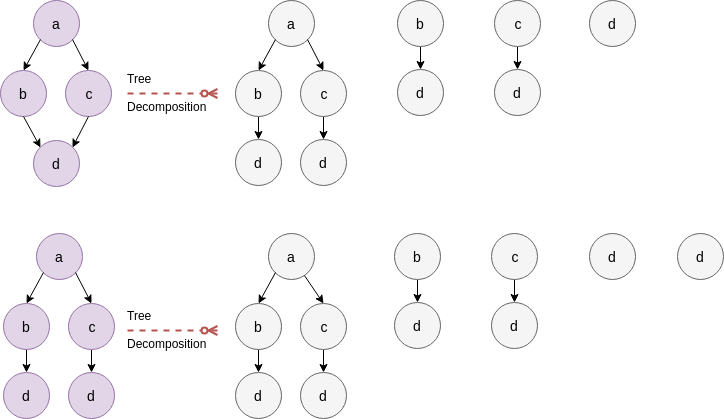
\includegraphics[width=\textwidth]{figures/odd_sth_2}
\caption[Επισκέψεις ταξινομημένων δέντρων μεταξύ δύο ΚΑΓ.]{Επισκέψεις ταξινομημένων δέντρων μεταξύ δύο ΚΑΓ. Προσέξτε ότι η δεύτερη περίπτωση διαφέρει από την πρώτη στη συχνότητα εμφάνισης του δέντρου-κόμβου \en{d}.}
\label{fig:odd_sth_2}
\end{figure}

Δεδομένης της παραπάνω σχέσης μερικής διάταξης μεταξύ των κόμβων ενός ΚΑΓ, μπορούμε να ορίσουμε μία νέα αποσύνθεση με διάταξη \en{ODD (Ordered Dag Decomposition} - Διατεταγμένη Αποσύνθεση ΚΑΓ), βάσει της οποίας όλα τα ΚΑΓ μπορούν να συνοψιστούν σε ένα μεγάλο ΚΑΓ που θα συμβολίζεται ως $BigDAG$.
Η μέθοδος αυτή που εισήχθει στο \cite[MinimalDAG: \tg{Σχήμα} 2, p. 3]{Martino2006}, συνοψίζει κόμβους με κοινές επισημειώσεις (μέσω ενός μετρητή συχνοτήτας εμφάνισης) αν ανήκουν στο ίδιο μονοπάτι του κάθε ΚΑΓ, ενώ συντηρεί και ενσωματώνει στο πλήρες γράφημα κόμβους για τους οποίους δεν βρέθηκε τρόπος να συνοψιστούν  (βλέπε σχήμα \ref{fig:odd_sth_3}).
Είναι δόκιμο να πούμε ότι το συνολικό $BigDAG$ μετράει τον αριθμό των υποδομών που ταυτίζονται μεταξύ των \en{ODD} ενός γράφου.
Λόγω της σχέσης μερικής διάταξης το παραγόμενο $BigDAG$ μας επιτρέπει να οδηγηθούμε στην παρακάτω ισοδυναμία:
\begin{equation}
K_{K_{DAG}}(G_{1}, G_{2}) = K_{BigDAG}(G_{1}, G_{2}) = \sum_{\substack{u_{1} \in V(BigDAG(G_{1}))\\ u_{2} \in V(BigDAG(G_{2})}} f_{u_{1}}f_{u_{2}}C(u_{1}, u_{2})
\end{equation}
όπου $f_{u}$ είναι ο μετρητής συχνότητας εμφάνισης του κόμβου $u$ και $C(u, v)$ είναι το πλήθος των γνήσιων υποδέντρων των δέντρων που ξεκινούν από τους κόμβους $u$ και $v$.
\begin{figure}[]
\centering
\includegraphics[width=0.8\textwidth]{figures/odd_sth_3}
\caption[Κατασκευή ενός $BigDAG$ από δύο επιμέρους ΚΑΓ.]{Κατασκευή ενός $BigDAG$ από δύο επιμέρους ΚΑΓ. Οι ακέραιοι αριθμοί στους κόμβους του $BigDAG$ αντιστοιχούν στις συχνότητες εμφάνισης τους.}
\label{fig:odd_sth_3}
\end{figure}

Τέλος έχοντας αναπαραστήσει κάθε γράφο ως ένα $BigDAG$, μπορούμε να συνοψίσουμε όλους τους γράφους σε ένα κοινό $Big^{2}DAG$ αν αντί να συνεχίσουμε να προσθέτουμε τις συχνότητες εμφάνισης των κόμβων όταν αυτοί τατίζονται, τις αντικαταστήσουμε με ένα διάνυσμα συχνοτήτων το οποίο έχει στην $i$-οστή θέση την τιμή $0$ αν ο κόμβος δεν εμφανίζεται στο $i$-οστό $BigDAG$ ενώ αλλιώς έχει για τιμή την συχνότητα εμφάνισης του (βλέπε σχήμα \ref{fig:odd_sth_4}).
\begin{figure}[]
\centering
\includegraphics[width=\textwidth]{figures/odd_sth_4}
\caption[Κατασκευή ενός $Big^{2}DAG$ από δύο επιμέρους $BigDAG$.]{Κατασκευή ενός $Big^{2}DAG$ από δύο επιμέρους $BigDAG$. Οι ακέραιοι αριθμοί αντικαθίστανται από διανύσματα συχνότητας που συγκρατούν την τιμή συχνότητας του κάθε κόμβου στο αρχικό $BigDAG$ ή δίνουν την τιμή $0$, στην περίπτωση που δεν υπήρχε.}
\label{fig:odd_sth_4}
\end{figure}

Στο τελικό $Big^{2}DAG$ γράφημα, ο υπολογισμός της μήτρας πυρήνα ανάγεται στον παρακάτω υπολογισμό:
\begin{equation}
K_{Big^{2}DAG}(G_{i}, G_{j}) = \sum_{u_{1}, u_{2} \in V(Big^{2}DAG)} F_{u_{1}}[i] \star F_{u_{2}}[j] C(u_{1}, u_{2})
\end{equation}
που είναι ισοδύναμος με:
\begin{equation}
K_{Big^{2}DAG}(G_{i}, G_{j}) = \sum_{u \in V(Big^{2}DAG)} F_{u}[i] \star F_{u}[j] C(u, u)
\end{equation}
επειδή ο πυρήνας υποδέντρων θα ταιριάξει μόνο στην περίπτωση που αυτά ταυτίζονται, δηλαδή:
\begin{equation}
C(u_{1}, u_{2}) \not= 0 \leftrightarrow T(u_{1}) = T(u_{2})
\end{equation}
Τέλος προκειμένου να κατασκευάσουμε το $Big^{2}DAG$ κάθε κόμβος θα πρέπει να αναπαρασταθεί σαν μία τούπλα $\langle D_{u} , F_{u}[\cdot], ID_{u} \rangle$ όπου με $D_{u}$ συμβολίζουμε το μέγεθος του υποδέντρου που ξεκινάει από τον κόμβο $u$, με $F_{u}[\cdot]$ το διάνυσμα συχνότητας εμφάνισης αυτού του κόμβου και με $ID_{u}$ ένα αλφαριθμητικό που μας χρησιμεύει προκειμένου να αναπαριστούμε αυτόν τον κόμβο \textbf{μοναδικά} (ιδιότητα που προκύπτει από την σχέση μερικής διάταξης).
Συγκεκριμένα:
\begin{equation}
ID_{u} = \begin{cases}
            L_{u},\;\text{αν}\;\delta^{+}(u)=0\\
            L_{u}(ID_{ch_{1}[u]}, \cdots, ID_{ch_{\delta^{+}(u)}[u]}),\;\text{αλλιώς}
        \end{cases}
\end{equation}
Προκειμένου να μειωθεί ακόμα περισσότερο ο χρόνος εκτέλεσης του αλγορίθμου μία προσέγγιση προτάθηκε, συγκεκριμένα αυτή του περιορισμού του βάθους εξερεύνησης των δέντρων \en{BFS} κατά την αποσύνθεση \en{ODD}, σε μία μέγιστη τιμή $h$.
Η θεωρητική πολυπλοκότητα του αλγορίθμου, θεωρώντας ότι το $h$ είναι σταθερό και παίρνει μικρές τιμές, είναι της τάξης του $\mathcal{O}(n\log n)$ \cite[\tg{Υποενότητα 5.5}]{Martino2012ATK}.

\subsection{Πυρήνας Διάδοσης}
\label{ssec:p2k}
Οι πυρήνες διάδοσης εισήχθησαν ως ένα γενικός σκελετός πυρήνα στο \cite{Neumann2016}.
Βασίζονται στην ιδέα της διάδοσης της πληροφορίας επισημείωσης μεταξύ κόμβων του γράφου, με βάση τη δομή του.
Κάθε γράφος θεωρείται ότι έχει συνεχείς επισημειώσεις στους κόμβους, όπου στην περίπτωση ύπαρξης διακριτών, αυτές μετασχηματίζονται σαν διανύσματα σταθερού μήκους όσο το μέγεθος του συνόλου των δυνατών επισημειώσεων και με άσους στην θέση που αντιστοιχεί στην αντίστοιχη επισημείωση (ήτοι \en{One-Hot-Vectors}).
Το σύνολο όλων των κόμβων ενός γράφου, μπορεί να ειδωθεί σαν μία κατανομή πιθανότητας $P$ μεγέθους $n \times d$, όπου το $n$ αντιστοιχεί στο νούμερο των κόμβων και το $d$ στη διάσταση των χαρακτηριστικών.
Έπειτα η ιδέα της διάδοσης εφαρμόζεται προκειμένου να κατασκευάσουμε ένα αλγοριθμικό σκελετό για τους πυρήνες διάδοσης.
Στην γενική του μορφή, ένας πυρήνας διάδοσης ακολουθεί τον σκελετό του αλγορίθμου \ref{alg:pk_generic}.
\selectlanguage{english}
\begin{algorithm}[]
\selectlanguage{greek}
\textbf{δεδομένα}: ένα σύνολο γράφων $\{G^{(i)}\}_{i}$, ένας αριθμός επαναλήψεων $t_{MAX}$, επαναληπτικό σχήμα διάδοσης, ένας πυρήνας βάσης $\langle\;.\;,\;. \rangle$
\\
\textbf{αρχικοποίηση}: $K \leftarrow 0$, αρχικοποίηση των κατανομών $P_{0}^{(i)}$.

\selectlanguage{english}
\For{$t \leftarrow 0 \dots t_{MAX}$}{
    \ForAll{\tg{τους γράφους} $G^{(i)}$}{
        \ForAll{\tg{τους κόμβους} $u \in G^{(i)}$}{
            \tg{κατακερμάτισε το} $p_{t, u}$ \tg{σε ομάδες}, \Comment*[r]{\tg{διάνυσμα με αριθμούς ομάδας}}
            \tg{όπου} $p_{t, u}$ \tg{είναι γραμμή του} $P^{(i)}_{t}$ \tg{που αντιστοιχεί στον κόμβο} $u$
        }
        \tg{υπολόγισε το} $\Phi_{i} = \phi(G_{t}^{i})$ \Comment*[r]{\tg{υπολόγισε πόσα στοιχεία ανήκουν σε κάθε ομάδα}}
    }
    $K \leftarrow K + \langle \Phi, \Phi \rangle$ \Comment*[r]{\tg{προσέθεσε την συνεισφορά αυτής της επανάληψης στον υπολογισμό πυρήνα}}
}
\ForAll{\tg{τους γράφους} $G^{(i)}$}{
    $P^{(i)}_{t+1} \leftarrow P_{t}^{(i)}$ \Comment*[r]{\tg{διάδωσε την πληροφορία του κάθε κόμβου}}

}
\caption{\tg{Υπολογισμός του γενικού πυρήνα διάδοσης}}
\label{alg:pk_generic}
\end{algorithm}
\selectlanguage{greek}

Ο υπολογισμός πυρήνα $\langle \Phi, \Phi \rangle_{ij}$, στην επανάληψη $t$ μεταξύ δύο γράφων $i, j$ είναι ισοδύναμος με το ακόλουθο διπλό άθροισμα:
\begin{equation}
    K(G^{(i)}_{t}, G^{(j)}_{t}) = \sum_{u \in G^{(i)}_{t}} \sum_{v \in G^{(j)}_{t}} k(u, v)
\end{equation}
όπου ο υπολογισμός του πυρήνα μεταξύ κόμβων $k(u, v)$, γίνεται μέσω ομαδοποίησης (\en{binning}).
Προκειμένου να ομαδοποιηθούν αποτελεσματικά οι κόμβοι, έπρεπε να βρεθεί μία μέθοδος που να είναι τόσο υπολογιστικά αποδοτική, όσο και εκφραστική.
Μία απλή συνάρτηση κατακερματισμού απορρίφθηκε, καθώς θα διαχώριζε τιμές που ήταν πολύ πιο \textit{όμοιες} μεταξύ τους σε σχέση με άλλες.
Μία έννοια \textit{τοπικότητας} έπρεπε να προστεθεί στην διαδικασία ομαδοποίησης, προκειμένου παρόμοια μοτίβα διάχυσης να μαζεύονται σε ίδιες ομάδες.
Για το σκοπό αυτό, χρησιμοποιήθηκε η τεχνική του τοπικά ευαίσθητου κατακερματισμού (\en{Locally Sensitive Hashing - \textbf{LSH}}) όπως φαίνεται στον αλγόριθμο \ref{alg:lsh}, για διάφορες μετρικές εγγύτητας, η οποία εφαρμόζεται συνολικά στην κατανομή πιθανότητας όλων των κόμβων, όλων των γράφων της εισόδου.
\selectlanguage{english}
\begin{algorithm}[]
\selectlanguage{greek}
\textbf{δεδομένα}: πίνακας $X \in \mathcal{R}^{N \times D}$, μέγεθος ομάδας $w$, μετρική $M$\\
\selectlanguage{english}
\If{$M = H$}{
    $X \leftarrow \sqrt{X}$ \Comment*[r]{\tg{μετασχηματισμός τετραγωνικής ρίζας}}
}
\If{$M=H\;\text{or}\; M=L2$ \Comment*[r]{\tg{δημιούργησε ένα τυχαίο διάνυσμα προβολής}}}{
    $v \leftarrow \text{RAND-NORM}(D)$ \Comment*[r]{\tg{πάρε τυχαία δείγματα από την $\mathcal{N}(0, 1)$}}
}
\ElseIf{$M = TV\;\text{or}\; M=L1$}{
    $v \leftarrow \text{RAND-NORM}(D)/\text{RAND-NORM}(D)$ \Comment*[r]{\tg{πάρε τυχαία δείγματα από την $\mathcal{C}auchy(0, 1)$}}
}
$b = w*\text{RAND-UNIF}()$ \Comment*[r]{\tg{τυχαίο διάνυσμα μετατόπισης $b \sim \mathcal{U}[0, w]$}}
$h(X) = \text{floor}((X*v + b)/w)$ \Comment*[r]{\tg{υπολόγισε τους κατακερματισμούς}}
\caption{\tg{Υπολογισμός του} LSH}
\label{alg:lsh}
\end{algorithm}
\selectlanguage{greek}

Όσο αφορά τον τρόπο διάδοσης, βάσει ενός πίνακα μετάβασης $T$ για κάθε γράφο, ο οποίος είναι κανονικοποιημένος κατά γραμμή, ένα επαναληπτικό σχήμα διάδοσης σχεδιάστηκε στη βάση του επόμενου απλού νόμου αντικατάστασης:
\begin{equation}
    P_{t+1} \leftarrow T P_{t}
\end{equation}
Ο πίνακας μετάδοσης $T$ είναι κατά κανόνα ίσος με $D^{-1}A$ για κάθε γράφο, όπου με $A$ συμβολίζουμε τον πίνακα γειτνίασης (βλέπε ορισμό \ref{def:adjacency_matrix}) αυτού του γράφου και $D = \text{\en{diag}}(\sum_{j} A_{ij})$.
Σχηματικό παράδειγμα τέτοιας προώθησης μπορεί να φανεί στo σχήμα \ref{fig:pk}.
Ο πυρήνας διάδοσης που τελικά υλοποιήσαμε στο πλαίσιο του \en{grakel} ακολουθεί τον αλγόριθμο \ref{alg:pk_imp}, ενώ στην περίπτωση μας θεωρούμε ότι οι γράφοι που μας δίνονται είναι \textit{πλήρως επισημειωμένοι}.
\selectlanguage{english}
\begin{algorithm}[ht!]
\selectlanguage{greek}
\textbf{δεδομένα}: ένα σύνολο γράφων $\{G^{(i)}\}_{i}$, ένας αριθμός επαναλήψεων $t_{MAX}$, πίνακας μετάδοσης $Τ$, μέγεθος ομάδας $w$, μετρική $M$, ένας πυρήνας βάσης $\langle.\;,\;. \rangle$\\
\textbf{αρχικοποίηση}: $K \leftarrow 0$, αρχικοποίηση των κατανομών $P_{0} \leftarrow \delta_{l(V)}$ (στην περίπτωση διακριτών επισημειώσεων) ή $P_{0} \leftarrow attr(V)$ στην περίπτωση των συνεχών.

\selectlanguage{english}
\For{$t \leftarrow 0 \cdots t_{MAX}$}{
    $\text{CALCULATE-LSH}(P_{t}, w, M)$ \Comment*[r]{\tg{ομαδοποίησε τους κόμβους}}
    \ForAll{\tg{τους γράφους} $G^{(i)}$}{
        \tg{Υπολόγισε το} $\Phi_{t} = \phi(G^{(i)}_{t})$ \Comment*[r]{\tg{μέτρησε το πλήθος των στοιχείων σε κάθε ομάδα}}
    }
    $ P_{t+1} \leftarrow T P_{t}$ \Comment*[r]{\tg{διάχυση επισημειώσεων}}
    $ K \leftarrow K + \langle \Phi,\; \Phi\rangle$ \Comment*[r]{\tg{προσέθεσε την συνεισφορά αυτής της επανάληψης στον υπολογισμό πυρήνα}}
}
\caption{\tg{Υπολογισμός του γενικού πυρήνα διάδοσης για πλήρως επισημειωμένους πυρήνες}}
\label{alg:pk_imp}
\end{algorithm}
\selectlanguage{greek}

\begin{figure}
\centering
  \begin{subfigure}[α]{1.0\linewidth}
    \centering\includegraphics[width=0.65\textwidth]{figures/pk1}
    \caption{Αρχική κατανομή επισημειώσεων ($t=0$)\label{fig:pk:a}}
  \end{subfigure}\\\vspace{1cm}
  \begin{subfigure}[β]{1.0\linewidth}
    \setlength{\abovecaptionskip}{0.3cm}
    \centering\includegraphics[width=0.7\textwidth]{figures/pk2}
    \caption{Ανανεωμένη κατανομή επισημειώσεων ($t=1$)\label{fig:pk:b}}
  \end{subfigure}
  \caption[Παράδειγμα εφαρμογής του αλγορίθμου προώθησης, με τοπικά ευαίσθητο κατακερματισμό, για δύο επαναλήψεις.]{Παράδειγμα εφαρμογής του αλγορίθμου προώθησης, με τοπικά ευαίσθητο κατακερματισμό, για δύο επαναλήψεις \ref{fig:pk:a}, \ref{fig:pk:b}.}
\label{fig:pk}
\end{figure}

%\begin{figure}
%\centering
%  \begin{subfigure}[α]{1.0\linewidth}
%    \centering\includegraphics[width=0.65\textwidth]{figures/pk1}
%    \caption{Αρχική κατανομή επισημειώσεων ($t=0$)\label{fig:pk:a}}
%  \end{subfigure}\\\vspace{1cm}
%  \begin{subfigure}[β]{1.0\linewidth}
%    \setlength{\abovecaptionskip}{0.3cm}
%    \centering\includegraphics[width=0.7\textwidth]{figures/pk2}
%    \caption{Ανανεωμένη κατανομή επισημειώσεων ($t=1$)\label{fig:pk:b}}
%  \end{subfigure}
%  \caption{Παράδειγμα εφαρμογής του αλγορίθμου προώθησης, με τοπικά ευαίσθητο κατακερματισμό, για δύο επαναλήψεις \ref{fig:pk:a}, %\ref{fig:pk:b}.}
%\label{fig:pk}
%\end{figure}
